



%Al fine di valutare se la scelta della tecnologia SiC-CsI può soddisfare le esigenze di NUMEN è stata implementata una simulazione Monte Carlo sulla piattaforma GEANT4.
%In questo capitolo vengono esposte le principali assunzioni e vengono presentati i risultati.



%Nei moderni esperimenti di fisica l'importanza delle simulazioni computerizzate è andata via via crescendo grazie all'eccezionale sviluppo dei computer e dei software volti a tale scopo; in particolare, l'introduzione delle tecniche Monte Carlo si è rivelata un potente strumento per trattare problemi complessi altrimenti difficilmente risolubili.
Nei moderni esperimenti di fisica l'importanza delle simulazioni numeriche è cresciuta senza sosta grazie all'eccezionale sviluppo dei computer e dei software di simulazione; in particolare, l'introduzione delle tecniche Monte Carlo si è rivelata un potente strumento per trattare problemi complessi altrimenti difficilmente risolubili.
In questo capitolo, dopo aver descritto le principali caratteristiche di tali metodi, si discute brevemente della piattaforma \geant.

%Successivamente, vengono presentati gli aspetti più importanti di tali simulazioni, le quali avevano lo scopo di valutare se la scelta di utilizzare dei telescopi basati sulla tecnologia SiC-CsI può soddisfare le esigenze di NUMEN.
%Successivamente, dopo aver presentato gli aspetti più importanti di tali simulazioni, vengono discussi i risultati ottenuti, illustrando nei diversi casi le matrici $\Delta E - E$ e calcolando la percentuale di errore nell'identificazione degli ioni simulati.
Successivamente, dopo aver spiegato gli aspetti più importanti del tool di simulazioni scritto per questo lavoro di tesi, vengono discussi i risultati ottenuti, evidenziando nei diversi casi le conseguenze sulle performance di Particle IDentification (PID) e sul rapporto segnale-fondo.



%Le simulazioni giocano un ruolo fondamentale nella fisica.

%In fisica, come in altre scienze, le simulazioni giocano un ruolo fondamentale, in quanto permettono di studiare la risposta di sistemi complessi tenendo sotto controllo alcuni dei suoi gradi di libertà.

\section{\iflanguage{italian}{Le simulazioni computerizzate e i metodi Monte Carlo}{Computer simulations and Monte-Carlo methods}}


In fisica, come in altre scienze, le simulazioni computerizzate giocano un ruolo fondamentale, in quanto permettono di affrontare lo studio di sistemi che sarebbero difficilmente trattabili utilizzando tecniche teoriche o sperimentali~``classiche'';
spesso, infatti, questi approcci possono presentare problematicità legate alla complessità del sistema, al tempo necessario per lo sviluppo e l'analisi, ai costi per la realizzazione di prototipi.
Introdotte negli anni Quaranta grazie all'apporto di prestigiosi scienziati come von Neumann, Ulam e Fermi, il loro progresso è stato parallelo a quello dei computer, arrivando oggi ad essere uno strumento imprescindibile in molti esperimenti.
%Esse forniscono una diversa prospettiva con cui guardare alla realtà, diventando in alcuni casi una base teorica da cui partire per l'interpretazione dei risultati sperimentali, oppure in altre situazioni producendo dati ``sperimentali'' con cui mettere al vaglio le teorie.
Esse forniscono una diversa prospettiva con cui guardare alla realtà, diventando in alcuni casi una base teorica da cui partire per l'interpretazione dei risultati sperimentali e in altri producendo dati ``sperimentali'' con cui mettere al vaglio le teorie.

Tra i diversi metodi di simulazione numerica, particolare importanza hanno assunto i cosiddetti \emph{metodi Monte Carlo}~\cite{metropolis:jasa49}, il cui nome fu coniato da Metropolis ispirandosi al casinò omonimo.
%Tali metodi utilizzano la generazione di sequenze di numeri \emph{pseudo-casuali} per simulare le fluttuazioni statistiche di un sistema con un numero elevato di gradi di libertà, 
%laddove i numeri pseudo-casuali sono dei numeri prodotti in modo deterministico ma con proprietà statistiche simili a quelle dei numeri casuali.
%
Il numero di problemi che al giorno d'oggi vengono studiati utilizzando questa tecnica è enorme, annoverando campi di ricerca estremamente diversi, che vanno dalla fisica nucleare alla fisica medica, dalla meccanica statistica alla sociofisica, dall'economia alla biologia.
%Darne una definizione comprensiva di tutte le aree di interesse è un compito difficile e sostanzialmente inutile.
%
% ***** QUESTO NON ERA MALE
%Sebbene darne una definizione comprensiva di tutte le aree di interesse sia un compito difficile, in generale è possibile dire che i metodi Monte Carlo utilizzano la generazione di numeri casuali per simulare le fluttuazioni statistiche di un sistema con un numero elevato di gradi di libertà accoppiati.
%
%
%Sebbene darne una definizione comprensiva di tutte le aree di interesse sia un compito difficile, in generale è possibile dire che i metodi Monte Carlo sono dei metodi numerici di risoluzione di equazioni o di calcolo di integrali basati sulla generazione di numeri casuali.
Sebbene darne una definizione comprensiva di tutte le aree di interesse sia un compito difficile, in generale è possibile dire che i metodi Monte Carlo sono dei metodi numerici, basati sulla generazione di numeri casuali, per la risoluzione di equazioni o per il calcolo di integrali.
%I metodi Monte Carlo utilizzano la generazione di numeri casuali per simulare le fluttuazioni statistiche di un sistema con un numero elevato di gradi di libertà.
Il generico metodo si compone principalmente di quattro fasi:
\begin{itemize}
	\item generazione di una sequenza di numeri casuali;
	\item calcolo delle variabili di input sulla base della sequenza estratta;
	\item determinazione delle variabili di output utilizzando le variabili di input calcolate;
	\item ripetizione dei punti precedenti e analisi critica dei risultati.
\end{itemize}



%Dal momento che i metodi Monte Carlo dipendono fortemente dalla produzione veloce ed efficiente di flussi di numeri casuali, si preferisce generare le sequenze di numeri via software, piuttosto che leggerli da tavole ad hoc.
%Tuttavia, poiché tali algoritmi sono, in realtà, deterministici, 
%In realtà, dal momento che, per ragioni di velocità ed efficienza, tali sequenze sono prodotte via software, i numeri sono \emph{pseudo-casuali}
%Per risolvere un problema complesso è necessaria una sequenza molto grande di numeri casuali, i quali devono essere indipendenti fra loro.
Affinché il metodo si dimostri efficace, è essenziale che la sequenza di numeri sia quanto più possibile casuale.
Dunque, proprio la casualità con cui vengono prodotti tali numeri rappresenta il punto più delicato del metodo; infatti, per ragioni di velocità ed efficienza, i numeri vengono generati via software invece di basarsi su processi fisici realmente casuali.
%Tuttavia, dal momento che tali algoritmi sono inevitabilmente deterministici, le sequenze di numeri sono, in realtà, \emph{pseudo-casuali}, ovvero presentano delle proprietà statistiche simili a quelle dei numeri casuali. 
Tuttavia, dal momento che tali algoritmi sono inevitabilmente deterministici, ogni numero della sequenza è univocamente calcolato a partire dal suo predecessore. 
Quindi, le sequenze di numeri sono, in realtà, \emph{pseudo-casuali}, ovvero presentano delle proprietà statistiche analoghe a quelle delle sequenze di numeri casuali, ma sono prodotte in modo deterministico. 
Per questo motivo, una successione di numeri pseudo-casuali non può avere elementi infinitamente diversi, in quanto, prima o poi, cominceranno a ripetersi.
Definendo \emph{periodo} il numero di iterazioni dopo le quali la successione si ripete, il problema legato alla pseudo-casualità della sequenza è ininfluente se il periodo è sufficientemente lungo rispetto al numero di eventi simulati.


Negli ultimi trent'anni l'importanza delle simulazioni basate su metodi Monte Carlo è cresciuta senza soluzione di continuità. 
%Uno dei motivi di tale successo deriva in quanto al crescere della complessità del problema tale tecnica risulta superiore rispetto agli approcci analitici in termini di tempo necessario per la 
%Uno dei motivi di tale successo deriva dalla maggiore efficacia di queste tecniche rispetto agli approcci analitici nella risoluzione di problemi caratterizzati da alta complessità;
%ad esempio, valutando l'efficacia di un metodo in termini del tempo necessario per risolvere un problema, al crescere della complessità risulta che tale tempo cresce più lentamente per i metodi Monte Carlo in confronto ai metodi analitici.
%come illustrato in Figura~\ref{fig:monte_carlo}, il tempo necessario 
%Uno dei motivi di tale successo deriva dalla grande efficacia di queste tecniche nella risoluzione di problemi altamente complessi;
Una delle ragioni di tale successo deriva dalla grande efficacia di queste tecniche nell'affrontare lo studio di sistemi con un numero elevato di gradi di libertà accoppiati. 
È possibile dimostrare che, al crescere della complessità del problema, i metodi Monte Carlo richiedono meno tempo per giungere alla soluzione rispetto alle tecniche analitiche o deterministiche, come mostrato in Figura~\ref{fig:monte_carlo}.


\begin{figure} [!t]
	\centering
	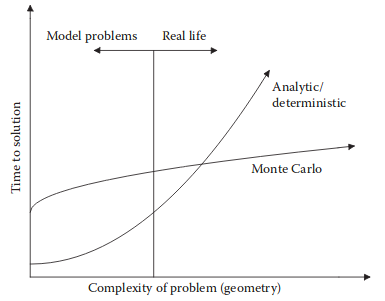
\includegraphics[scale=0.66]{Grafici/monte_carlo_vs_analytic2.png}
	\caption{Confronto fra il tempo necessario per la risoluzione di un problema con un metodo analitico-deterministico e con un metodo Monte Carlo, al variare della complessità del problema. Figura tratta da~\cite{bielajew:13}.} \label{fig:monte_carlo}
\end{figure}


%Nel campo della fisica, i metodi Monte Carlo sono spesso utilizzati per 
%Un notevole impulso allo sviluppo dei metodi Monte Carlo è provenuto dalla fisica delle alte energie, in cui l'elevata complessità degli apparati di rivelazione necessitava di uno strumento per decidere le specifiche in fase di progettazione.


%Un notevole impulso allo sviluppo dei metodi Monte Carlo è provenuto dalla fisica delle alte energie, in cui la crescente necessità di simulare complessi sistemi di rivelazione spingeva per la realizzazione di software sempre più performanti e robusti.
%
% ***** PRIMA AVEVO MESSO QUESTA
%Un notevole impulso allo sviluppo dei metodi Monte Carlo è provenuto dalla fisica delle alte energie, in cui si comprese che tali metodi offrivano la possibilità di seguire la traccia delle particelle e simulare le loro interazioni con la materia.
%
Un notevole impulso allo sviluppo delle tecniche di simulazione è provenuto dalla fisica delle alte energie, in cui si comprese che tali strumenti, offrendo la possibilità di seguire le tracce delle particelle ed ``imitare'' le loro interazioni con la materia, potevano essere impiegati sia per la progettazione dei rivelatori sia per lo studio della loro risposta nelle condizioni sperimentali di interesse.
In questo contesto nacque il codice \emph{GEANT}, di cui nella sezione successiva si espongono le principali caratteristiche.





%\section{\iflanguage{italian}{La piattaforma \textsc{Geant4}}{\textsc{Geant4} toolkit}}

\section{\iflanguage{italian}{La piattaforma Geant4}{Geant4 toolkit}}

%\section{\textsc{Geant4}}

La piattaforma GEANT, il cui nome deriva da \emph{GEometry ANd Tracking}, fu sviluppata nel 1974 al CERN di Ginevra allo scopo di simulare l'interazione di particelle elementari ad alta energia con i rivelatori.
%Questa prima versione consentiva di simulare il trasporto di un numero ristretto di particelle 
%In questa prima versione era possibile simulare soltanto un numero ristretto di particelle
In questa prima versione era possibile considerare soltanto un numero ristretto di particelle e forme geometriche semplici. 
Nel 1982 venne distribuito GEANT3, scritto in FORTRAN e nettamente potenziato rispetto al suo predecessore; infatti, si potevano simulare apparati sperimentali grandi e sofisticati e fasci di particelle molto energetici.
Tuttavia, il codice presentava una struttura molto complessa, che rendeva difficile l'introduzione di nuove caratteristiche o la ricerca di errori.
%the simulation software geant4, which means \emph{geometry and tracking}, is a toolkit based on
%Fu così che si arrivò al 1998, anno dell'uscita dell'ultima versione del codice, chiamata \geant, interamente basata sul linguaggio C++.
%La crescente necessità di simulare complessi sistemi di rivelazione spingeva per la realizzazione di software sempre più performanti e robusti.
%
%%Fu così che nel 1998, grazie alla collaborazione di oltre 40 istituti internazionali, venne pubblicata l'ultima versione del codice, chiamata \geant.
D'altro canto, la crescente necessità di simulare complessi sistemi di rivelazione spingeva per la realizzazione di software sempre più performanti e robusti.
Fu così che nel 1998, grazie alla collaborazione di oltre 40~istituti internazionali, venne pubblicato un nuovo progetto, chiamato~\geant.
Esso è interamente basato sul linguaggio C++, traendo vantaggio, dunque, da tutte le potenzialità offerte da una tecnologia orientata agli oggetti, come ad esempio la modularità e la compattezza.
% oppure il polimorfismo
%Il modo più corretto di definire \geant{} è \emph{toolkit}, ovvero ``cassetta per gli attrezzi'', in quanto comprende un insieme di librerie software che l'utente può selezionare a seconda delle proprie esigenze per creare un'applicazione specifica.

Oggi \geant{} consente di simulare l'interazione con la materia di tutte le particelle note, in un range energetico che va da pochi~eV fino ai~TeV.
%
%La sua notevole duttilità lo ha reso uno strumento 
Grazie alla sua notevole duttilità, sono innumerevoli gli esperimenti che si avvalgono di questo strumento: la sua area d'azione comprende la fisica delle alte energie, la fisica nucleare, le applicazioni in campo medico e l'astrofisica.
Il codice è, inoltre, open-source e viene periodicamente aggiornato dalla collaborazione. 
Dal momento che la documentazione su \geant{} è ampia e dettagliata\footnote{Si veda, ad esempio, \url{www.geant4.org}.}, nel prosieguo vengono presentati soltanto gli aspetti utili alla comprensione delle simulazioni svolte per questo lavoro di tesi.  



%\subsection{\iflanguage{italian}{La struttura di \textsc{Geant4}}{\textsc{Geant4} structure}}

\subsection{\iflanguage{italian}{La struttura di Geant4}{Geant4 structure}}

%Il modo più corretto di definire \geant{} è \emph{toolkit}, ovvero ``cassetta per gli attrezzi'', in quanto comprende un insieme di librerie software che l'utente può selezionare a seconda delle proprie esigenze per creare un'applicazione specifica.
Il modo più corretto di definire \geant{} è \emph{toolkit}, ovvero ``cassetta per gli attrezzi'', in quanto è costituito da un insieme di librerie software che, a seconda delle esigenze, possono essere selezionate per creare un'applicazione specifica.
L'utente deve, quindi, scrivere la sua applicazione, definendo tutti i parametri rilevanti: alcuni devono essere inseriti in modo obbligatorio, altri possono essere aggiunti facoltativamente.
%\geant{} offre numerose funzionalità:

%Ogni simulazione si compone dei seguenti aspetti: 
Nella progettazione e nella realizzazione del software, tutti gli aspetti fondamentali di un processo di simulazione sono stati inclusi:
\begin{itemize}
	\item la geometria del sistema, specificando forma, dimensione e posizione dei vari oggetti;
	\item i materiali utilizzati;
	\item la sorgente delle particelle, di cui si definisce la posizione, l'energia, la distribuzione angolare e tutte le altre caratteristiche rilevanti;
	\item i processi fisici di interazione per la modellizzazione  del comportamento delle particelle;
	%\item il tracciamento delle particelle, che può essere calcolato anche passo dopo passo, consentendo di estrarre ad ogni step informazioni legate alla particella, come ad esempio energia e posizione;
	\item il tracciamento delle particelle attraverso materiali ed, eventualmente, campi elettromagnetici esterni;
	%\item la sensitività di un rivelatore e la sua risposta;
	\item la definizione di elementi sensibili, che simulano la risposta del rivelatore;
	\item la visualizzazione tridimensionale degli oggetti simulati e delle tracce delle particelle;
	\item la generazione di dati, i quali possono essere memorizzati per una successiva analisi.
\end{itemize}


%Ciascuno degli aspetti elencati corrisponde ad una determinata \emph{classe} o \emph{categoria}, che, agendo in modo indipendente l'una dall'altra, danno al software una struttura modulare.

Gli aspetti elencati corrispondono in \geant{} a determinate \emph{classi} o \emph{categorie}, che, agendo in modo indipendente l'una dall'altra, danno al software una struttura modulare.
%Esse sono state concepite per essere facilmente estendibili o modificabili dall'utente, seguendo la logica tipica dei linguaggi orientati agli oggetti;
Esse sono state concepite per essere facilmente estendibili o modificabili, seguendo la logica tipica dei linguaggi orientati agli oggetti; infatti, grazie ad un approccio basato sul \emph{polimorfismo} e sull'\emph{ereditarietà}, l'utente può fornire un'implementazione alternativa delle funzioni presenti in una categoria.
%Esse sono state concepite per essere facilmente estendibili o modificabili, seguendo la logica tipica dei linguaggi orientati agli oggetti; \geant{} usa, infatti, un approccio basato sulle proprietà del \emph{polimorfismo} e dell'\emph{ereditarietà}.
%Di tutte le classi messe a disposizione, \geant{} richiede obbligatoriamente l'implementazione e l'istanziazione di tre, ovvero 
%\geant mette a disposizione un grande numero di classi, le quali sono state  concepite per essere facilmente estendibili o modificabili dall'utente, seguendo la logica tipica dei linguaggi orientati agli oggetti.
%L'implementazione e l'istanziazione di queste classi sono obbligatorie in tre casi, ovvero
%\geant{} mette a disposizione un grande numero di classi, ma per tre di loro l'implementazione e l'istanziazione sono obbligatorie.
\geant{} mette a disposizione un grande numero di classi, richiedendo obbligatoriamente l'implementazione e l'istanziazione per tre di loro: 
\begin{itemize}
	\item la classe dedicata alla definizione della geometria e dei materiali;
	\item la classe prevista per la definizione delle particelle, dei processi fisici e delle soglie per la produzione dei secondari;
	\item la classe rivolta alla generazione delle particelle primarie.
\end{itemize}


%Altre classi

Le altre classi sono, invece, opzionali e, a seconda delle esigenze, l'utente può modificarne il comportamento di default definendo la propria ``versione''; 
%ad esempio, ai fini di questo lavoro è stato necessario personalizzare la classe che rappresenta ogni ``passo'' della traccia della particella, facendo in modo che ad ogni step venisse estratta l'informazione sulla perdita di energia e sulla posizione.
%
ad esempio, in \geant{} esiste una classe che rappresenta ogni ``passo'' (più propriamente chiamato \emph{step}) della traccia di una particella, sia essa primaria o secondaria.
%, laddove per passo possiamo immaginare un segmento che compone la traiettoria.
L'utente può personalizzare la funzione che accede alle informazioni dello step (chiamata \emph{UserSteppingAction}), facendo in modo che ad ogni step vengano, ad esempio, estratte la posizione e l'energia della particella.
%In \geant{} la traccia della particella è divisa in \emph{step}, che, per comodità, possiamo immaginare come dei segmenti.
%Grazie ad un'apposita classe, è possibile accedere a diverse informazioni legate a tale step, come estremi 


\section{\iflanguage{italian}{Gli aspetti principali della simulazione}{Simulation main aspects}}

%La simulazione implementata per questo lavoro di tesi considera una matrice di telescopi SiC-CsI.
%Allo scopo di valutare le prestazioni di PID
Nell'ambito di questo lavoro di tesi è stata realizzata un'applicazione in \geant{} per simulare la risposta di un sistema di telescopi SiC-CsI agli ioni di interesse per il progetto NUMEN.
Nel seguito di questa sezione vengono illustrate nel dettaglio le caratteristiche di tale applicazione.




\subsection{\iflanguage{italian}{La geometria e i materiali}{Geometry and materials}} \label{par:geometria}

Ciascun telescopio è formato da due stadi, il rivelatore al carburo di silicio (SiC) e il cristallo allo ioduro di cesio (CsI), i quali sono posti a contatto.
Per tenere in considerazione il substrato morto del rivelatore al SiC, il primo stadio è, a sua volta, costituito da due parti: il volume attivo e il substrato morto.

Considerando un sistema di riferimento in cui l'asse $z$ è individuato dalla direzione di propagazione delle particelle, i telescopi sono fra loro separati di 2~mm lungo la direzione $x$ e di 1~mm lungo la direzione $y$.

%Ciascun telescopio è formato da tre parti: il volume attivo del rivelatore al SiC, il substrato morto dello stesso rivelatore e il cristallo allo CsI.

%In accordo con le 
%
%Un importante aspetto della simulazione riguarda lo spessore dei rivelatori.


%Dal momento che nuovi sviluppi tecnologici hanno reso possibile la rimozione quasi totale del substrato, sono state svolte anche delle simulazioni in cui il suo spessore era ridotto a 10~$\mu$m. 
%Per quanto riguarda il cristallo di CsI, lo spessore è stato posto uguale a 1~cm.


%Poiché uno degli obiettivi di questo lavoro consisteva nella ricerca delle migliori condizioni di granularità,  sono stati considerati diversi valori per le dimensioni trasversali; in particolare, sulla base degli attuali limiti imposti dal processo di produzione dei rivelatori al SiC, sono state simulate aree sensibili di $1 \times 1$, $1.5 \times 1.5$ e $2 \times 2$~cm\ap{2}.
%Poiché uno degli obiettivi di questo lavoro consisteva nella ricerca delle migliori condizioni di granularità,  per le dimensioni trasversali dei telescopi sono stati presi in esame diversi valori; in particolare, sulla base degli attuali limiti imposti dal processo di produzione dei rivelatori al SiC, sono state simulate aree sensibili di $1 \times 1$, $1.5 \times 1.5$ e $2 \times 2$~cm\ap{2}.
Poiché uno degli obiettivi principali di questo lavoro consisteva nella ricerca delle condizioni ottimali di granularità, sono state condotte diverse simulazioni al variare delle dimensioni trasversali dei telescopi; in particolare, sulla base degli attuali limiti imposti dal processo di produzione dei rivelatori al SiC, sono state simulate aree sensibili di $1 \times 1$, $1.5 \times 1.5$ e $2 \times 2$~cm\ap{2}.




%Lo spessore del primo è di 100~$\mu$m, mentre quello del secondo è di 350~$\mu$m.
%Un altro aspetto importante della simulazione riguarda lo spessore del rivelatore al SiC; infatti, sebbene la collaborazione abbia suggerito 
%Per quanto riguarda lo spessore dei due stadi del telescopio, la collaborazione aveva individuato come probabile soluzione l'utilizzo di rivelatori al SiC da 100~$\mu$m e di cristalli allo CsI di 1~cm. 

%Lo standard tecnologico attuale prevede che un rivelatore al SiC di tale spessore abbia un substrato morto spesso 350~$\mu$m.
Per quanto riguarda lo spessore dei due stadi del telescopio, in accordo con la soluzione individuata dalla collaborazione, sono stati simulati rivelatori al~SiC da 100~$\mu$m e cristalli allo CsI da 1~cm, mentre per il substrato morto si è considerato un valore di 350~$\mu$m.
%Gli spessori tenuti in considerazione erano di 100~$\mu$m per il rivelatore al SiC, di 350~$\mu$m per il substrato morto e di 1~cm per il cristallo allo CsI.
%Tuttavia, dal momento che nuovi sviluppi tecnologici hanno reso possibile la rimozione quasi totale degli strati morti, si è esaminato anche il caso in cui lo spessore del substrato fosse ridotto a 10~$\mu$m. 
%È stato, dunque, effettuato un confronto tra le diverse condizioni, al fine di valutarne le conseguenze sulle capacità di~PID.





%Sebbene il muro di telescopi comprenderà oltre 1000 
%La simulazione ha considerato un unico modulo di $2 \times 5$ rivelatore.

%%Dal momento che per gli scopi di questo lavoro non era necessario includere l'intero muro di 1230 telescopi, tutte le simulazioni sono state svolte prendendo in esame una matrice di $2 \times 5$ elementi.

In Figura~\ref{fig:simulazione_muro} è mostrato l'aspetto assunto da un modulo elementare di~$2 \times 5$ telescopi nella simulazione \geant. 
Dal momento che allo scopo di valutare le capacità di PID del sistema non è necessario includere l'intero muro di rivelatori, tutte le simulazioni sono state svolte considerando un solo telescopio.
%In Figura~ è possibile vedere la realizzazione grafica di \geant{} di un modulo $2 \times 5$ del sistema di rivelazione.

\begin{figure} [!p]
	\centering
	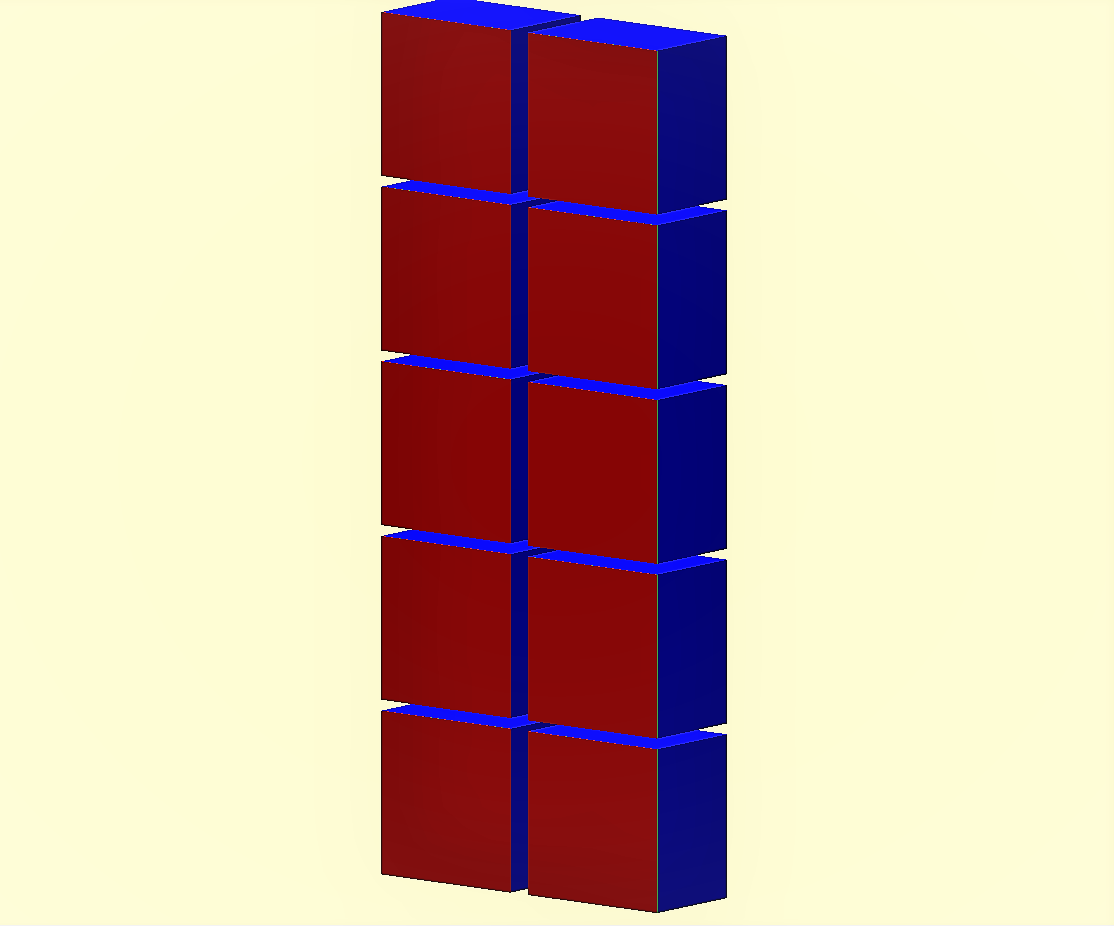
\includegraphics[width=\textwidth, keepaspectratio]{Grafici/modulo2_ritagliato.png}
	\caption{Una matrice di $2 \times 5$ telescopi: in rosso il rivelatore al SiC, in verde, appena visibile, il substrato morto di tale rivelatore e in blu il cristallo allo CsI.} \label{fig:simulazione_muro}
\end{figure}


\subsection{\iflanguage{italian}{La generazione delle particelle primarie}{Primary particles generation}} \label{par:particelle_primarie}

%Le particelle primarie simulate comprendono tre degli ioni di maggiore interesse per NUMEN, ovvero \ce{^{18}O}, \ce{^{18}F} e \ce{^{18}Ne}. 
%In alcune simulazioni sono stati coinvolti anche altri isotopi di tali specie nucleari, 
%Le particelle primarie simulate comprendono tre degli ioni di maggiore interesse per NUMEN, ovvero \ce{^{18}O}, \ce{^{18}F} e \ce{^{18}Ne}, coinvolgendo in alcune simulazioni anche altri isotopi di tali specie atomiche, quali \ce{^{16}O}, \ce{^{17}O}, \ce{^{19}F}, \ce{^{20}F}, \ce{^{19}Ne} e \ce{^{20}Ne}.
In una simulazione \geant{} i parametri che tipicamente devono essere introdotti per la generazione di un evento sono: la tipologia della particella primaria, la sua energia cinetica iniziale, la sua direzione iniziale e la sua posizione iniziale.
%In questo paragrafo verranno spiegate le condizioni di lavoro scelte in merito a tali parametri.
In questo paragrafo verranno spiegate le scelte effettuate in merito a tali parametri.
%(\textcolor{red}{Lo tolgo questo paragrafetto?})

Le particelle primarie simulate comprendono sette degli ioni di maggiore interesse per NUMEN, ovvero \ce{^{20}O^{8+}}, \ce{^{21}O^{8+}}, \ce{^{20}F^{8+}}, \ce{^{21}F^{8+}}, \ce{^{20}Ne^{8+}}, \ce{^{21}Ne^{8+}} e \ce{^{22}Ne^{8+}}; il primo, in particolare, rappresenta lo ione di interesse nello studio di una classe di reazioni di DCE, mentre gli altri costituiscono le principali sorgenti di fondo.
%In alcuni casi esaminati gli ioni sono stati considerati completamente ionizzati, mentre in altri sono stati simulati diversi stati di carica.

%In ciascun evento, la particella primaria è stata generata in modo casuale sulla faccia anteriore del rivelatore al SiC centrale, con una direzione estratta casualmente all'interno di un angolo solido corrispondente ad un cono con un'apertura di~20\textdegree{}. 
%Poiché il sistema che si intende analizzare è posto nel piano focale di uno spettrometro magnetico, l'energia e la 
%Affinché gli eventi simulati potessero riprodurre fedelmente gli eventi reali, 
%al fine di riprodurre fedelmente gli eventi reali

%Poiché il sistema che si intende analizzare è posto nel piano focale di uno spettrometro magnetico, è stato necessario introdurre una correlazione tra la posizione di impatto delle particelle sul telescopio e la loro energia cinetica; infatti, nella situazione reale gli eiettili prodotti nell'interazione fra il fascio di particelle e il bersaglio attraversano il quadrupolo e il dipolo 

%Per quanto riguarda l'energia iniziale delle particelle primarie, bisogna ricordare che 


%Poiché il sistema che si intende analizzare sarà posto nel piano focale di uno spettrometro magnetico, l'energia delle particelle primarie deve essere correlata alla loro posizione di arrivo sul piano focale; infatti, nell'apparato sperimentale reale, gli eiettili, attraversando il dipolo, subiranno una deflessione dovuta alla forza di Lorentz. 

% la forza di Lorentz stabilisce la relazione 
%la quale definisce la traiettoria della particella fissandone il raggio di curvatura $\rho$.

%Poiché il sistema che si intende analizzare sarà posto nel piano focale di uno spettrometro magnetico, è stato necessario introdurre una correlazione tra la posizione di arrivo delle particelle sul piano focale e la loro energia cinetica; 
%Poiché il sistema che si intende analizzare sarà posto nel piano focale di uno spettrometro magnetico, l'energia cinetica delle particelle simulate non può essere indipendente dalla loro posizione di arrivo sul piano focale, ma deve essere introdotta una correlazione fra queste quantità;
Le energie cinetiche simulate devono essere scelte tenendo in considerazione che negli spettrometri magnetici gli ioni vengono separati in base alla loro \emph{rigidità magnetica} $B \rho$; infatti, quando una particella con carica~$q$ e massa $m$ si muove in un campo magnetico~$B$ ortogonale al suo impulso~$p$, a causa della forza di Lorentz essa descrive una traiettoria con raggio di curvatura~$\rho$, dato dalla nota relazione
\begin{equation} \label{eq:legge_spettrometri}
B  \rho \, = \,  \frac{p}{q}
\end{equation}
%In approssimazione non relativistica, l'impulso $p$ è legato all'energia cinetica $E$ dalla relazione $p = \sqrt{2 m E}$, laddove $m$ indica massa della particella; dunque, la precedente può essere scritta nella forma
%\begin{equation} \label{eq:legge_spettrometri_energia}
% \rho \, \propto \,  \frac{\sqrt{m}}{q} \sqrt{E}
%\end{equation}
%La~\ref{eq:legge_spettrometri_energia} afferma che 
Al primo ordine di approssimazione, $\rho$ è proporzionale a $x_{foc}$, coordinata orizzontale del punto di arrivo della particella sul piano focale.
Inoltre, in approssimazione non relativistica, l'impulso $p$ è legato all'energia cinetica $E$ dalla formula $p = \sqrt{2 m E}$. 
Esiste, dunque, una relazione fra $x_{foc}$ ed $E$: essa è circa quadratica e dipende dal rapporto $\sqrt{m}/q$, ovvero
\begin{equation} \label{eq:legge_spettrometri_approx}
B \, x_{foc} \, \propto \,  \frac{\sqrt{m}}{q} \sqrt{E}
\end{equation}
%La~\ref{eq:legge_spettrometri_approx} afferma che ioni uguali, emessi ad angoli differenti con energie cinetiche uguali, giungono sullo stesso punto del piano focale; equivalentemente, ioni uguali, emessi allo stesso angolo con energie cinetiche differenti, giungono su punti diversi del piano focale.
La~\ref{eq:legge_spettrometri_approx} afferma che ioni con la stessa rigidità magnetica giungono sullo stesso punto del piano focale; equivalentemente, ioni con diversa rigidità magnetica giungono su punti diversi del piano focale.
Quanto appena detto è illustrato in Figura~\ref{fig:magnex_diverse_traiettorie}, la quale mostra una simulazione GEANT di MAGNEX per diverse traiettorie accettate dallo spettrometro.
\begin{figure} [!t]
	\centering
	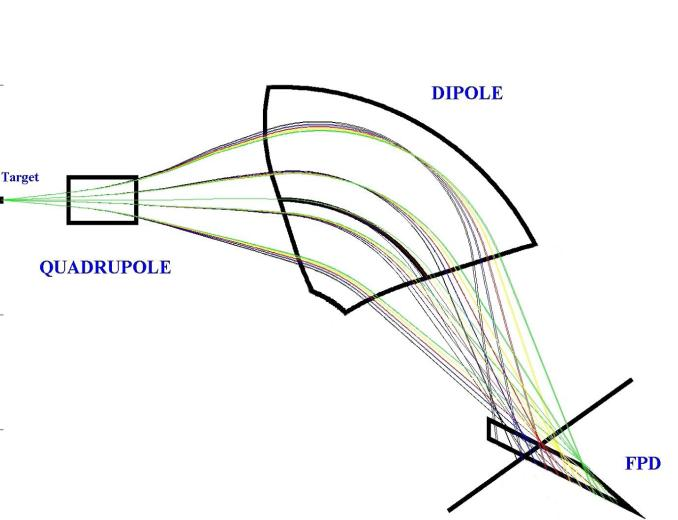
\includegraphics[width=\textwidth, keepaspectratio]{Grafici/magnex_traiettorie_diverse.png}
	\caption{Simulazione GEANT di MAGNEX: traiettorie con colori differenti hanno energie diverse. Figura tratta da~\cite{cappuzzello:epja16}.} \label{fig:magnex_diverse_traiettorie}
\end{figure}



A causa della estensione finita dei rivelatori, in realtà gli ioni arrivano sul telescopio in una finestra di valori di $B \rho$. La larghezza di tale finestra è data, al primo ordine, da
\begin{equation} \label{eq:finestra_Brho}
	\Delta \left(B \rho \right) \sim \frac{\Delta x}{D}
\end{equation} 
laddove $\Delta x$ indica l'estensione lungo la direzione dispersiva del rivelatore e $D$ è la dispersione in impulso dello spettrometro, pari a 3.68~cm/\%.

La dipendenza della \ref{eq:legge_spettrometri_approx} dal rapporto $\sqrt{m}/q$ costituisce il fondamento di un'innovativa tecnica di identificazione per spettrometri di grande accettanza; se, infatti, si misurano in correlazione la posizione $x_{foc}$ e l'energia cinetica~$E$, è possibile identificare gli ioni in massa e stato di carica.
L'applicazione di tale tecnica allo spettrometro MAGNEX è stata ampiamente discussa in numerose pubblicazioni, alle quali si rimanda per informazioni più dettagliate (si veda ad esempio~\cite{cappuzzello:nima10}). 

Dal momento che la simulazione deve riflettere il comportamento reale degli ioni nello spettrometro, è stato necessario introdurre le suddette correlazioni energia-posizione. 
Inoltre, la cinematica delle reazioni nucleari introduce ulteriori correlazioni fra l'energia cinetica e l'angolo di emissione dell'eiettile.
Entrambi questi fattori sono caratterizzati da effetti non-lineari particolarmente importanti per MAGNEX a causa della grande accettanza in angolo solido ($\sim 50$~msr ) e impulso ($ +10\% \div -14\%$). 
Tali distorsioni difficilmente possono essere inseriti direttamente nella simulazione \geant. 
%A tal fine si è scelto di utilizzare i software dedicati al trasporto ottico dei prodotti di reazione attraverso gli elementi magnetici dello spettrometro. 
Per questo motivo si è scelto di determinare tali correlazioni mediante software sviluppati all'uopo e ottimizzati dalla collaborazione NUMEN.
%Poiché all'interno della collaborazione NUMEN erano già stati sviluppati e ottimizzati dei software dedicati al calcolo della cinematica di reazione e al trasporto ottico degli eiettili attraverso gli elementi magnetici dello spettrometro, si è scelto di   
Tali software sono basati sugli algoritmi di COSY INFINITY~\cite{makino:nima99} e utilizzano il formalismo dell'algebra differenziale per risolvere le equazioni del moto dei prodotti di reazione fino al decimo ordine~\cite{cappuzzello:epja16}.
Scegliendo la tipologia e l'energia della reazione nucleare di interesse, essi determinano la cinematica di reazione e lo spazio delle fasi iniziale; dopo di che calcolano la matrice del trasporto ad alto ordine e ricostruiscono il moto degli eiettili fino all'ingresso del rivelatore di piano focale (Focal Plane Detector, FPD).
%Scegliendo lo spazio delle fasi iniziale, essi ricostruiscono il moto degli eiettili fino all'ingresso del rivelatore di piano focale (Focal Plane Detector, FPD), permettendo di conoscere alcune osservabili fondamentali, come l'energia cinetica~$E$, la posizione~$(x_{foc},y_{foc})$ e gli angoli~$(\theta_{foc},\phi_{foc})$ di incidenza. 
%Queste osservabili sono date in input alla simulazione \geant{}, la quale descrive dunque l'interazione degli ioni con il telescopio.
Questi software producono in output un file contenente i valori delle osservabili rilevanti, come ad esempio l'energia cinetica~$E$, la posizione~$(x_{foc},y_{foc})$ e gli angoli di incidenza~$(\theta_{foc},\phi_{foc})$ sul FPD.
La simulazione \geant{} è stata realizzata in modo da prendere in input tali dati e, a partire da questi, ricavare tutte le informazioni necessarie per la generazione degli eventi; in altre parole, ad ogni particella primaria vengono assegnate un'energia cinetica iniziale, una posizione iniziale e una direzione iniziale generate da COSY INFINITY.
%I software per il trasporto tracciano gli ioni fino all'ingresso del FPD 
Rispetto all'ingresso del FPD, il telescopio è posto ad una distanza di 14~cm, in quanto nell'apparato sperimentale reale tale spazio è occupato dal tracciatore a~gas. 
Attualmente la simulazione non comprende tale rivelatore, per cui gli ioni percorrono un tratto nel vuoto.
L'integrazione tra i software dedicati al trasporto ottico e la simulazione \geant{} è stata fondamentale per riprodurre correttamente le condizioni operative reali dello spettrometro.

Per valutare le capacità di PID del telescopio è necessario che tutti gli ioni simulati incidano sul dispositivo simulato. 
In base a quanto detto precedentemente, essi devono dunque avere la stessa finestra di $B \rho$, che comporta energie cinetiche differenti per i diversi ioni. 
Fissato un valore di riferimento per la rigidità magnetica, grazie ai software per il trasporto è stato possibile determinare, per ogni ione, l'intervallo di energia cinetica corrispondente al range di $B \rho$ accettato dal telescopio.
%per ogni ione è stata determinata l'energia cinetica corrispondente a tale valore e 
%Fissato un valore di rigidità magnetica di riferimento, per ogni ione è stata determinata l'energia cinetica corrispondente a tale valore e, attorno a tale valore, è stato considerato un intervallo di energia cinetica di 10~MeV, in modo da coprire la 



%Per introdurre le correlazioni energia-posizione, si è scelto di utilizzare i software dedicati al trasporto ottico dei prodotti di reazione attraverso lo spettrometro magnetico. 


%Allo scopo di coprire un ampio range energetico, realisticamente significativo per NUMEN, le particelle primarie hanno un'energia scelta casualmente fra 500 e 1000~MeV.
%%Allo scopo di valutare la capacità di PID in un ampio range energetico, realisticamente significativo per NUMEN, sono state simulate particelle primarie con un'energia scelta casualmente fra 500 e 1000~MeV.
%Dal momento che l'apparato sperimentale si incardina sulle proprietà dello spettrometro magnetico MAGNEX, 

%%È bene ricordare che negli spettrometri magnetici la posizione di una particella al piano focale è correlata alla sua energia; infatti, partendo dalla nota relazione
%\begin{equation} 
%B  \rho \, = \,  \frac{p}{q} \, 
%\end{equation}
%laddove $B$ è il campo magnetico, mentre $\rho$, $p$ e $q$ sono, rispettivamente, il raggio di curvatura, l'impulso e la carica della particella, sotto opportune condizioni è possibile affermare che\footnote{La relazione $p = \sqrt{2 m E}$ vale in approssimazione non relativistica.}
%\begin{equation} 
%B x_{foc} \, \approx \, B  \rho  \, \propto \,  \frac{\sqrt{m}}{q} \sqrt{E_{resid}}
%\end{equation}
%Dunque, per tenere in considerazione questo aspetto, alcune simulazioni sono state svolte tenendo fissata la rigidità magnetica $B \rho$ degli ioni primari e variandone in corrispondenza l'energia.
%Inoltre, dal momento che negli spettrometri magnetici la posizione di una particella al piano focale è correlata alla sua energia, in accordo con la nota relazione
%\begin{equation} \label{eq:legge_spettrometri}
%B  \rho \, = \,  \frac{p}{q}
%\end{equation}
%laddove $B$ è il campo magnetico, mentre $\rho$, $p$ e $q$ sono, rispettivamente, il raggio di curvatura, l'impulso e la carica della particella, alcune simulazioni sono state svolte tenendo fissato la rigidità magnetica $B \rho$ degli ioni primari.



\subsection{\iflanguage{italian}{I processi fisici}{Physics processes}}


Affinché la simulazione possa riprodurre con la maggiore accuratezza possibile i risultati sperimentali reali, è di cruciale importanza la scelta dei processi fisici da considerare allo scopo di definire il comportamento delle particelle.
Per gli scopi di questo lavoro, in una prima fase sono state prese in esame soltanto le interazioni elettromagnetiche (oltre ai processi di decadimento e di decadimento radioattivo), preponderanti nell'interazione ione-rivelatore alle energie di interesse.
I processi di ionizzazione, in particolare, sono alla base delle tecniche di PID basate sulla perdita di energia degli ioni nella materia dei rivelatori.
Successivamente, sono state aggiunte anche le interazioni adroniche, incorporando, dunque, processi di scattering elastico e inelastico e meccanismi di reazioni nucleari.

In Figura~\ref{fig:simulazione_evento} è riportata la visualizzazione grafica della simulazione di 20~eventi nel caso in cui il modello dei processi fisici comprendesse sia le interazioni elettromagnetiche sia quelle adroniche: in nero sono raffigurate le tracce degli ioni primari, mentre con altri colori sono mostrate le tracce delle particelle secondarie originate da reazioni nucleari. 



\begin{figure} [!p]
	\centering
	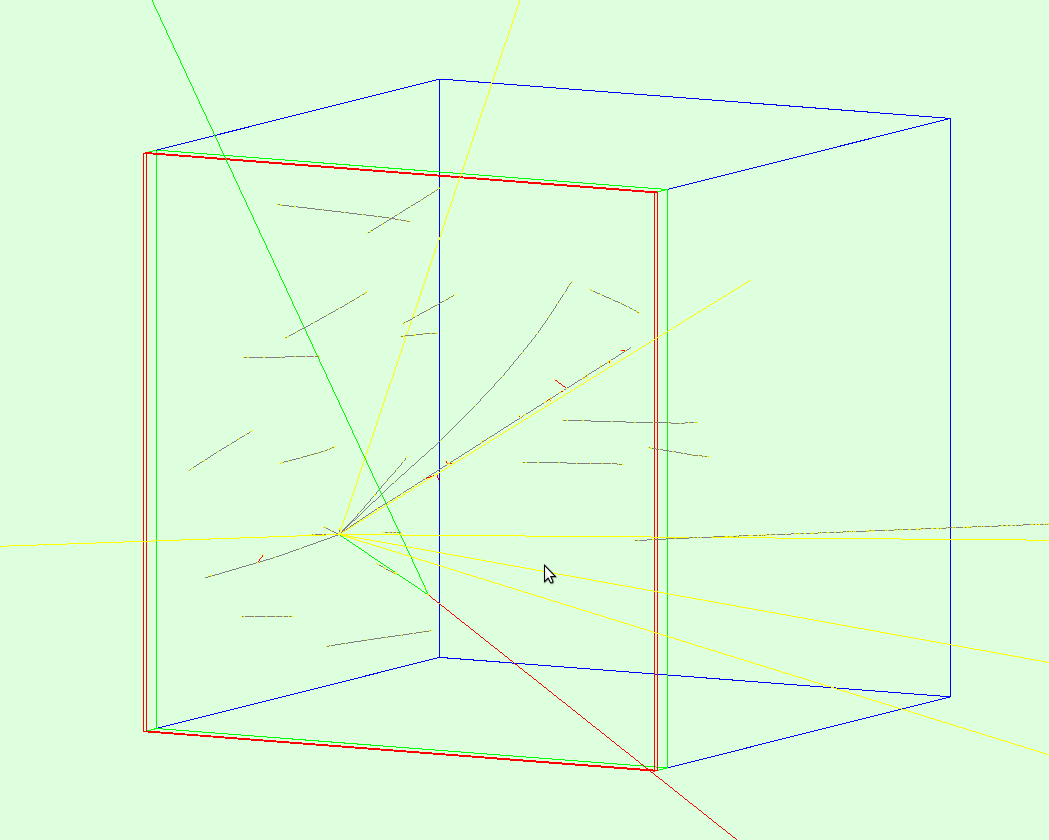
\includegraphics[width=\textwidth, keepaspectratio]{Grafici/evento5_ritagliato.png}
	\caption{Rappresentazione grafica della simulazione di 20~eventi: in nero le tracce degli ioni primari (\ce{^{18}O}), in altri colori le tracce delle particelle secondarie prodotte da reazioni nucleari con i nuclei del mezzo: dal momento che riescono ad uscire fuori dal rivelatore, si tratta, probabilmente, di particelle leggere, come protoni, neutroni e particelle $\alpha$.} \label{fig:simulazione_evento}
\end{figure}




%Non sono state modificate le impostazioni di default di
Una delle componenti fondamentali di \geant{} riguarda la scelta dei parametri di cut-off.
È possibile definire una soglia in range: elettroni di ionizzazione e gamma di bremsstrahlung aventi un range inferiore alla soglia non vengono generati esplicitamente, ma la loro energia viene considerata essere un deposito locale.
Dal momento che, ai fini di questo lavoro, una modifica dei parametri di cut-off non avrebbe portato a significativi cambiamenti dei risultati, si è scelto di mantenere le impostazioni di default, che corrispondono ad un range di 1~mm.



\subsection{\iflanguage{italian}{Tracciamento delle particelle}{Particles step}}

%In \geant{} la traccia della particella è divisa in \emph{step}, che, per comodità, possiamo immaginare come dei segmenti.
%Grazie ad un'apposita classe, è possibile accedere a diverse informazioni legate a tale step.
Come anticipato nella sezione precedente, in \geant{} è possibile modificare il comportamente della funzione UserSteppingAction.
Dal momento che, ai fini di questo lavoro, si volevano valutare le conseguenze sulla PID causate dagli effetti di bordo dei rivelatori, era necessario sapere punto per punto la posizione dello ione. 
Dunque, è stato modificato il comportamento di questa classe, affinché ad ogni step si conoscessero la posizione e il deposito di energia; in particolare, dal momento che \geant{} permette di conoscere gli estremi dello step, si è scelto di far corrispondere le coordinate del deposito di energia a quelle di un punto estratto in modo casuale sul segmento congiungente i due estremi.








\subsection{\iflanguage{italian}{Elaborazione post-simulazione}{Post-simulation processing}}

I dati prodotti dalla simulazione, scritti in un TTree di ROOT~\cite{brun:nima97}, sono stati elaborati da una macro di ROOT, grazie alla quale sono state aggiunte alcune caratteristiche tipiche dei rivelatori reali e sono stati ricostruiti gli spettri energetici.
%In primo luogo, ciascun deposito di energia viene pesato con una funzione di r
%In primo luogo, dal momento che 
%
%In primo luogo, a causa del processo di produzione, i rivelatori al SiC presentano nel volume sensibile un bordo esterno completamente inattivo, dove la carica generata per ionizzazione non viene raccolta, ed una regione di transizione, in cui la carica prodotta viene raccolta soltanto in parte.
In primo luogo, a causa del processo di produzione, i rivelatori al SiC presentano attorno al volume sensibile un bordo esterno completamente inattivo ed una regione di transizione: nel primo la carica generata per ionizzazione non viene raccolta, nella seconda viene raccolta soltanto in parte.
Secondo le misurazioni effettuate, la zona totalmente morta ha una lunghezza di circa 200~$\mu$m, mentre la regione di transizione ha un'estensione di circa 50~$\mu$m. 
%Nella macro si è tenuto conto di tali \emph{effetti di bordo} pesando ciascun deposito di energia con una \emph{funzione di risposta} lineare, che nel caso unidimensionale sarebbe così definita: 
%\begin{equation}
%f(x) =
%\begin{cases}
%1        & \quad  x<a \\
%\alpha x & \quad  b<x<a\\
%0        & \quad  x>b
%\end{cases}
%\end{equation}
%
Nella macro si è tenuto conto degli \emph{effetti di bordo} pesando ciascun deposito di energia con una \emph{funzione di risposta} così definita: nella zona interamente attiva era pari ad uno, nella regione di transizione decresceva linearmente e nella zona del tutto inattiva aveva valore nullo.
Un grafico esemplificativo dell'andamento di tale funzione nel caso unidimensionale è riportato in Figura~\ref{fig:funzione_risposta}.


\begin{figure} [!p]
	\centering
	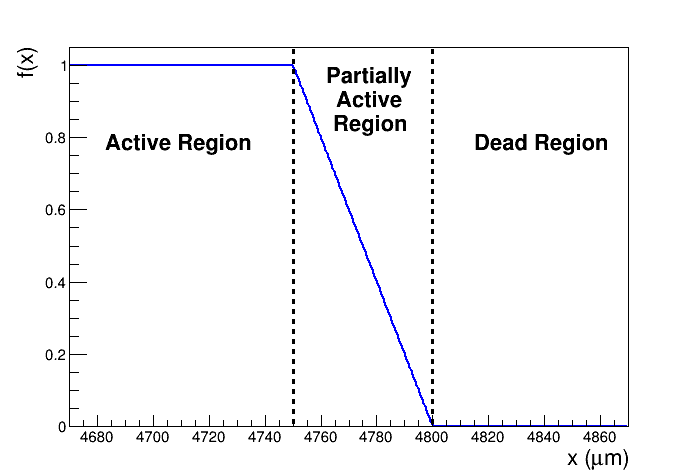
\includegraphics[width=\textwidth, keepaspectratio]{Grafici_Tesi/Funzione/funzione.png}
	\caption{L'andamento della funzione di risposta $f(x)$ assunta per descrivere gli effetti di bordo del rivelatore al SiC.} \label{fig:funzione_risposta}
\end{figure}

%Nella macro, inoltre, sommando le diverse perdite di energia, per ogni evento veniva ricostruito il deposito energetico totale nel rivelatore al SiC e nel cristallo allo CsI.
Nella macro, inoltre, sommando step dopo step l'energia persa dallo ione, per ogni evento è stata ricostruita l'energia rilasciata nel rivelatore al SiC e quella depositata nel cristallo allo CsI.
Registrando, evento per evento, tutti i depositi di energia, si sono riprodotti gli spettri energetici degli ioni per entrambi gli stadi del telescopio.
A questo livello, soltanto le fluttuazioni statistiche legate alla ionizzazione sono tenute in considerazione.
Dunque, al fine di riprodurre le risoluzioni energetiche tipiche dei rivelatori in esame, lo spettro energetico è stato ``allargato'' campionando ciascun deposito di energia con una distribuzione gaussiana, la cui espressione è
%\begin{equation}
%	f(E) = A \, \mbox{e}^{- \frac{E - E_0}{2 {\sigma}^2}}
%\end{equation}
\begin{equation}
	f(E, E_0, \sigma) = \frac{1}{\sqrt{2 \pi \sigma^2}} \, \exp \left[ - \frac{ \left(E - E_0 \right)^2}{2 {\sigma}^2}  \right]
\end{equation}
dove $E_0$ è il valore originario del deposito di energia, $E$ è il valore dopo il campionamento e $\sigma$ è la deviazione standard.
Di tale distribuzione, noto il valore medio $E_0$, bisognava scegliere la $\sigma$ in modo tale che la risoluzione energetica ricavata dalla simulazione fosse confrontabile con quella sperimentale.
%Dal momento che la risoluzione energetica è generalmente espressa come la somma in quadratura di un termine legato alle fluttuazioni statistiche del numero dei portatori e di uno dovuto al rumore elettronico, nella macro si è parametrizzata la $\sigma$ nel modo seguente
La risoluzione energetica è generalmente espressa come la somma in quadratura di un termine legato alle fluttuazioni statistiche del numero dei portatori, proporzionale a $E^{-1/2}$, e di uno dovuto al rumore elettronico, proporzionale a $E^{-1}$~\cite{knoll:10}.
Dunque, dal momento che la $\sigma$ può essere messa in relazione alla risoluzione energetica $R$ attraverso la~formula
\begin{equation}
	R \,  = \, \frac{\mbox{FWHM}}{E} \, = \, \frac{2.35 \, \sigma}{E}
\end{equation}
nella macro si è parametrizzata la deviazione standard nel modo seguente
\begin{equation}
\sigma = \sqrt{a + b \, E}
\end{equation}
laddove $a$ e $b$ sono due costanti.
%che assumono valori diversi a seconda che si consideri il rivelatore al SiC o il cristallo allo CsI. 
Nella somma al secondo membro, il primo addendo corrisponde al termine legato al rumore elettronico, mentre il secondo rappresenta quello causato dalle fluttuazioni del numero di portatori.
%
%
%Ricordando che la FWHM è legata alla $\sigma$ dalla relazione
%\begin{equation}
%\mbox{FWHM} = 2.35 \, \sigma
%\end{equation}
%la deviazione standard risulta collegata alla risoluzione energetica.
%Dal momento che quest'ultima è generalmente determinata dalla somma in quadratura di un termine legato all
Scegliendo opportuni valori per $a$ e $b$, si è assunta per il rivelatore al SiC una risoluzione energetica intrinseca dello 0.8\% FWHM a 25.3~MeV, mentre per il rivelatore allo CsI del 2\% FWHM a 700~MeV, in affinità con i valori tipici di questi dispositivi a tali energie. 







%\clearpage


\section{\iflanguage{italian}{I risultati}{Results}}

In questa sezione vengono presentati i risultati ottenuti dal tool di simulazioni elaborato per questo lavoro di tesi.
Poiché l'obiettivo principale di questo lavoro consiste nella valutazione delle prestazioni di PID di tale sistema, la maggior parte delle simulazioni ha lo scopo di stimare il rapporto segnale-fondo che si avrebbe nell'identificazione degli ioni di interesse.

È bene ricordare che la tecnica $\Delta E - E$ prevede la correlazione fra la perdita di energia $\Delta E$ e l'energia cinetica totale $E$. In riferimento al caso in esame, $\Delta E$ corrisponde all'energia persa dalla particella primaria nel rivelatore al~SiC (che da ora in poi indicheremo con $ \Delta E_{SiC}$), mentre $E$ equivale alla sua energia cinetica iniziale. Nelle simulazioni svolte, quest'ultima quantità è data da
\begin{equation}
	E \, = \, \Delta E_{SiC} + E_{sub} + E_{CsI}
\end{equation}
laddove $E_{sub}$ è l'energia persa nel substrato morto ed $E_{CsI}$ è l'energia residua rilasciata nel cristallo allo CsI.
In realtà, $E_{sub}$ non sarebbe sperimentalmente accessibile; di conseguenza, per tenere conto delle energie realmente misurabili, bisogna introdurre la quantità $E_{meas}$, definita nel modo seguente
\begin{equation}
	E_{meas} \, = \, \Delta E_{SiC} + E_{CsI}
\end{equation}

%Dal momento che uno degli aspetti studiati in questo lavoro consiste nel valutare la differenza fra la correlazione $\Delta E - E_{tot}$ e quella $\Delta E - E_{resid}$, per maggiore chiarezza nel prosieguo verrà specificato se  
Inoltre, dal momento che uno degli aspetti studiati in questo lavoro consiste nel valutare se la correlazione $\Delta E_{SiC} - E_{CsI}$ può garantire prestazioni analoghe a quella $\Delta E_{SiC} - E_{meas}$, nel prosieguo verrà specificato quale tipo di correlazione si sta considerando.
%Dunque, dal momento che nel prosieguo verrà valutata la differenza fra le matrici 

%Per semplicità della trattazione si è preferito suddividere la sezione in paragrafi specifici, evidenziando di volta in volta quali parametri sono stati variati e quali sono stati tenuti fissi.
%Tenendo in mente questo obiettivo, per semplicità della trattazione si è preferito esporre i risultati evidenziando di volta in volta quali parametri sono stati variati e quali sono stati tenuti fissi.
Per semplicità della trattazione si è preferito esporre i risultati in modo schematico, evidenziando di volta in volta quali parametri sono stati variati e quali sono stati tenuti fissi.

%\subsection{\iflanguage{italian}{Caso ideale}{Ideal case}}
\subsection{\iflanguage{italian}{Particelle monocromatiche, ortogonali e centrali }{Monochromatic, orthogonal and central particles}}


Come primo esempio si è scelto di illustrare i risultati di un caso ideale in cui le particelle primarie sono generate con un'energia di 800~MeV ed incidono ortogonalmente e centralmente al telescopio, il quale ha, in questo caso, dimensioni trasversali di 1.5~cm $\times$ 1.5~cm.
%Il substrato epitassiale ha una lunghezza di 350~$\mu$m.
Per semplicità gli ioni considerati sono soltanto \ce{^{20}O}, \ce{^{20}F} e \ce{^{20}Ne}.
Nella prima fase di implementazione della simulazione, il modello dei processi fisici utilizzato prendeva in considerazione soltanto le interazioni elettromagnetiche, i processi di decadimento e di decadimento radioattivo.
Dal momento che la formula di Bethe-Bloch è ricavata tenendo conto della sola interazione elettromagnetica, il modello adottato è sufficiente per studiare l'identificazione di ioni diversi nelle matrici $\Delta E_{SiC} - E_{meas}$.
Questa affermazione viene confermata dalla Figura~\ref{fig:deltaE_ETot}, in cui è possibile notare che i luoghi determinati da eventi associati all'interazione di ioni di \ce{^{20}O}, \ce{^{20}F} e \ce{^{20}Ne} con il telescopio sono chiaramente distinti.
\begin{figure} [!t]
	\centering
	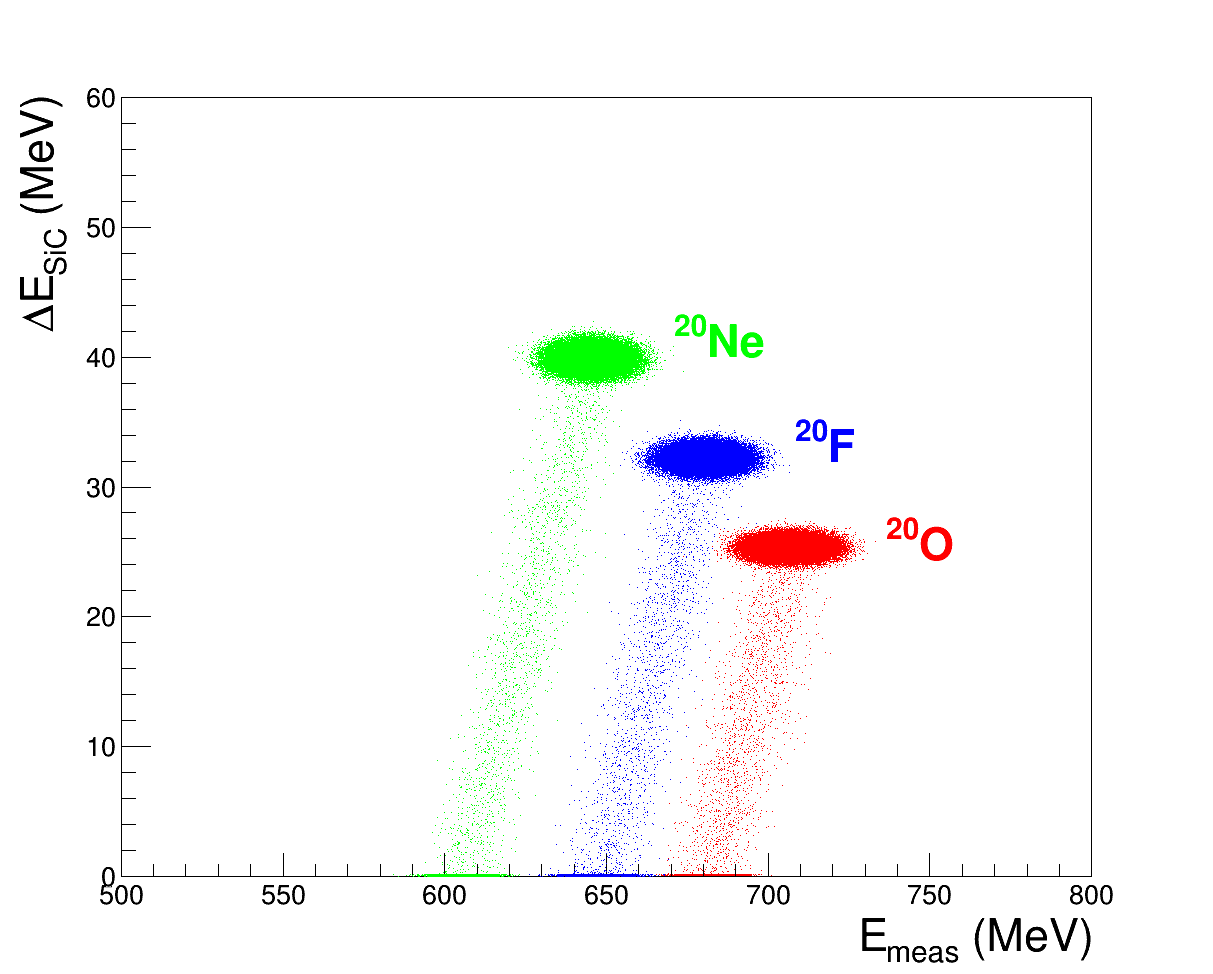
\includegraphics[width=\textwidth, keepaspectratio]{Grafici_Tesi2/Particelle_monocromatiche/deltaE_ETot_quadrata.png}
	\caption{Matrici $\Delta E_{SiC} - E_{meas}$ per \ce{^{20}O}, \ce{^{20}F} e \ce{^{20}Ne} con particelle monocromatiche, ortogonali e centrali.} \label{fig:deltaE_ETot}
\end{figure}
In particolare, essi si dispongono ad $E_{meas}$ diverse perché la parte di energia persa nel substrato morto dipende dal numero atomico ($Z$) dello ione.
In secondo luogo, si fa notare che al di sotto di ogni addensamento sono presenti degli eventi in cui l'energia residua è stata misurata correttamente, mentre la perdita di energia risulta inferiore al valore ``corretto'': si tratta di eventi in cui la carica prodotta nel rivelatore al SiC è stata raccolta parzialmente. 
Tali eventi costituiscono una delle principali sorgenti di fondo nella PID, in quanto potrebbero disporsi sul luogo caratteristico di uno ione diverso, ed essere erroneamente attribuiti ad uno~$Z$ sbagliato.
Inoltre, essi costituiscono una perdita di segnali corretti che deve essere minimizzata, in particolar modo se si intende studiare processi estremamente rari come quelli di DCE.
Si deduce, quindi, che per avere delle buone capacità di PID è essenziale che la frazione di questi eventi rispetto al totale sia piccola.











In Figura~\ref{fig:deltaE_Tot} e in Figura~\ref{fig:ETot} sono riportate, rispettivamente, le proiezioni sull'asse $\Delta E_{SiC}$ e sull'asse $E_{meas}$ delle matrici $\Delta E_{SiC} - E_{meas}$: esse rappresentano gli spettri energetici misurati dal rivelatore al SiC e da quello allo~CsI.
Effettuando un fit gaussiano sul picco dell'\ce{^{20}O} nello spettro di $\Delta E_{SiC}$, si trova una FWHM di 1.1~MeV, corrispondente ad una risoluzione del 4.5\%.
Poiché questo valore è ben più grande della risoluzione intrinseca assunta per tale rivelatore, si deduce che in questo caso la componente più significativa della risoluzione compete alle fluttuazioni nel processo di ionizzazione.

\begin{figure} [!p]
	\centering
	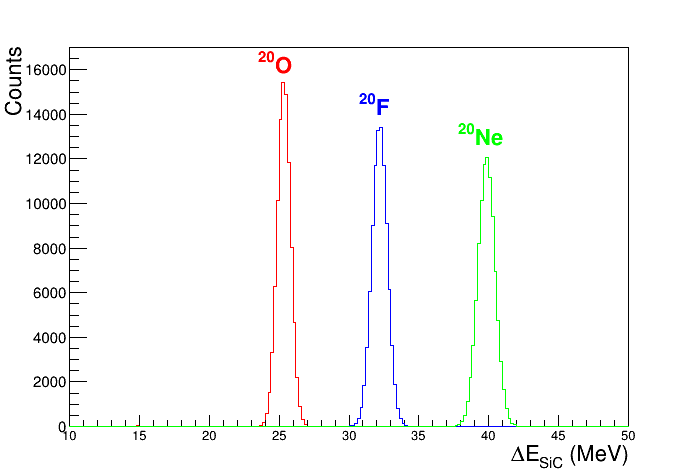
\includegraphics[scale=0.5]{Grafici_Tesi2/Particelle_monocromatiche/deltaE.png}
	\caption{Spettro in $ \Delta E_{SiC} $.} \label{fig:deltaE_Tot}
\end{figure}


\begin{figure} [!p]
	\centering
	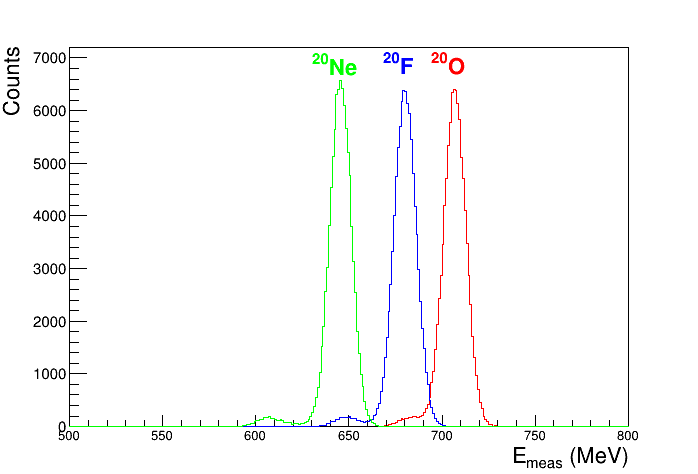
\includegraphics[scale=0.5]{Grafici_Tesi2/Particelle_monocromatiche/ETot.png}
	\caption{Spettro in $E_{meas} = \Delta E_{SiC} + E_{CsI}$.} \label{fig:ETot}
\end{figure}







%\vspace{1cm}

%\subsection{\iflanguage{italian}{Processi fisici senza interazioni adroniche}{Physics process without adronic interactions}}
\subsection{\iflanguage{italian}{Particelle monocromatiche, non ortogonali e non centrali }{Not monochromatic, not orthogonal and not central particles}} \label{par:particelle_non_monocromatiche}







In questo secondo esempio ideale le particelle primarie hanno sempre un'energia di 800~MeV, ma la loro posizione iniziale è estratta casualmente sulla faccia di ingresso del rivelatore al SiC centrale e la direzione del loro impulso varia in modo casuale in un cono di apertura di 20\textdegree{}.
Anche in questo caso viene utilizzato il modello dei processi fisici dell'esempio precedente, così come per la geometria e le dimensioni dei telescopi.
%La geometria e le dimensioni dei telescopi restano, invece, uguali a quelle dell'esempio precedente.
Le corrispondenti matrici $\Delta E_{SiC} - E_{meas}$ sono rappresentate in Figura~\ref{fig:deltaE_ETot_full_energy}.
\begin{figure} [!p]
	\centering
	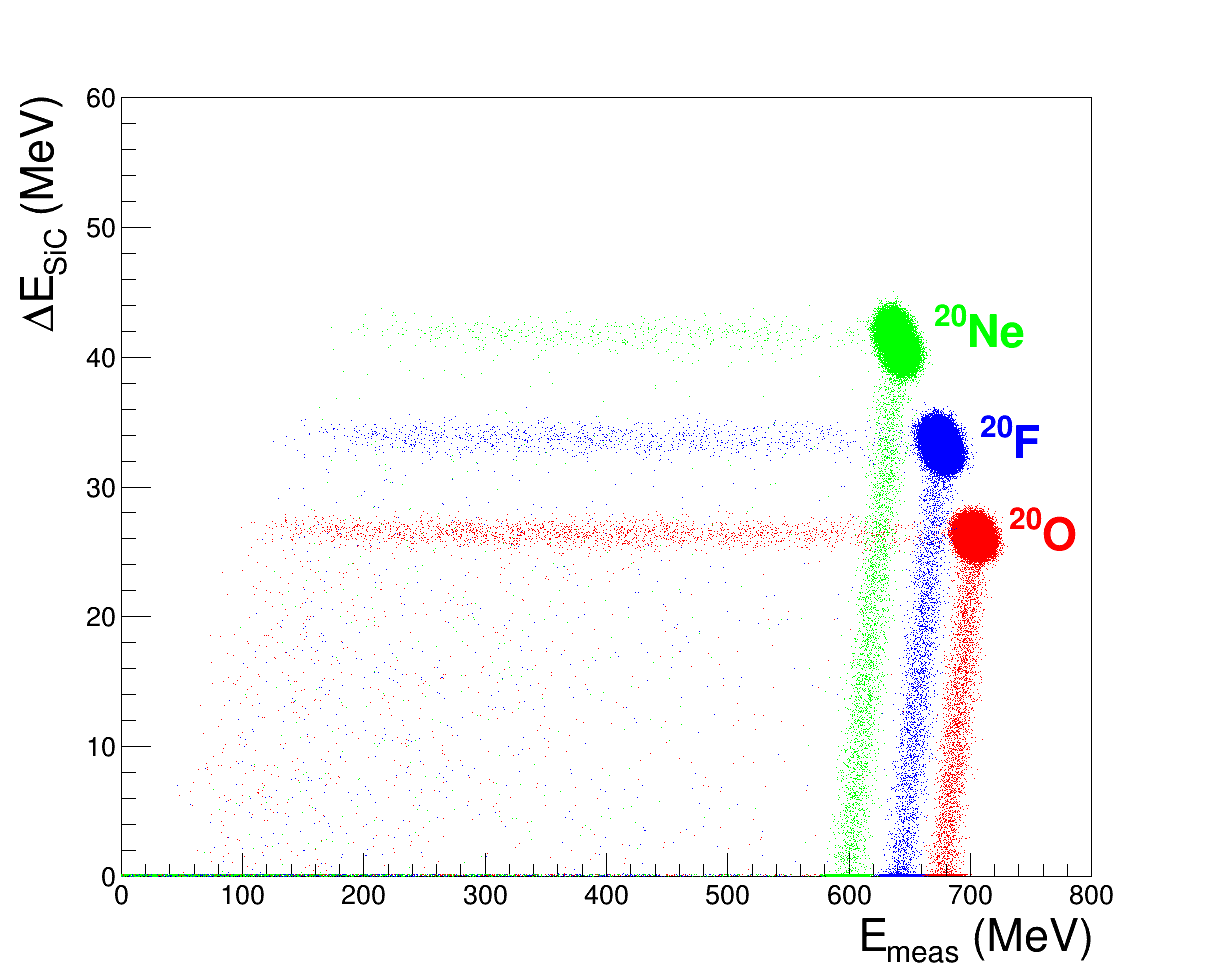
\includegraphics[width=\textwidth, keepaspectratio]{Grafici_Tesi2/Particelle_non_ortogonali/deltaE_ETot_intero_range_quadrata.png}
	\caption{Matrici $\Delta E_{SiC} - E_{meas}$ con particelle monocromatiche, non ortogonali e non centrali.} \label{fig:deltaE_ETot_full_energy}
\end{figure}
%Inoltre, a differenza del caso precedente si nota la comparsa di eventi in cui la perdita di energia $\Delta E_{SiC}$ viene misurata correttamente, mentre l'energia $E_{tot}$ ha un valore inferiore rispetto a quello ``corretto''.
Rispetto al caso precedente, fanno la loro comparsa degli eventi in cui la perdita di energia $\Delta E_{SiC}$ viene misurata correttamente, mentre l'energia $E_{meas}$ ha un valore inferiore rispetto a quello corretto. 
Ciò dipende da quegli eventi in cui le particelle escono fuori dal cristallo di~CsI, non rilasciando totalmente la loro energia residua.
A causa del motivo precedentemente citato, anche questi eventi introducono una componente di fondo nella PID e una perdita di segnali corretti.
Per meglio comprendere l'entità degli eventi degradati, sono riportate in Figura~\ref{fig:fetta} le proiezioni sull'asse verticale e su quello orizzontale della matrice: come si può notare, tali eventi costituiscono un continuo che si estende fino a zero e rendono leggermente asimmetriche le distribuzioni.
\begin{figure} [!p]
	\centering
	\subfigure[]
	{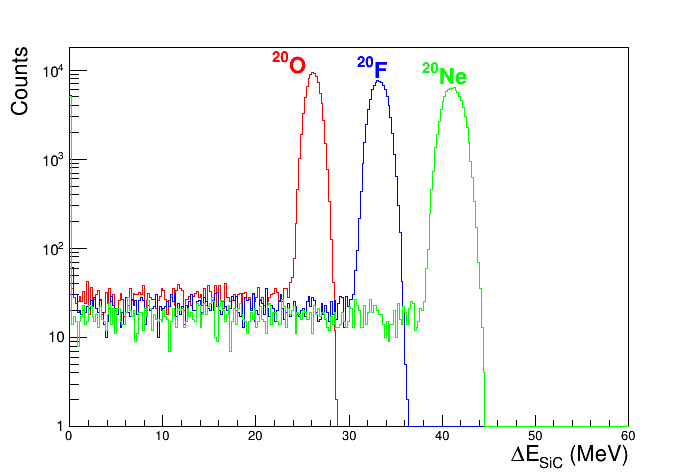
\includegraphics[scale=0.479]{Grafici_Tesi2/Particelle_non_ortogonali/deltaE.png}}
	%\vspace{7mm}
	\subfigure[]
	{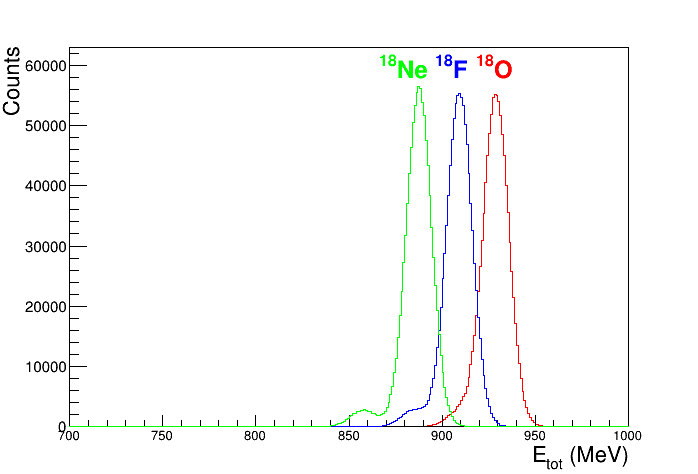
\includegraphics[scale=0.479]{Grafici_Tesi2/Particelle_non_ortogonali/ETot.png}}
	
	\caption{Le proiezioni delle matrici $\Delta E_{SiC} - E_{meas}$ di Figura~\ref{fig:deltaE_ETot_full_energy}: in (a) sull'asse $\Delta E_{SiC}$, in (b) sull'asse $E_{meas}$.} \label{fig:fetta}
\end{figure} 
In Figura~\ref{fig:fetta}.b si può, inoltre, osservare un secondo picco situato ad un valore di $E_{meas}$ di poco inferiore a quello assunto nel picco principale; esso è dovuto agli ioni che attraversano la cornice completamente inattiva attorno al rivelatore al~SiC, rilasciando una quantità di energia che non viene misurata.
%Allo scopo di dare una stima quantitativa della frazione di nuclei potenzialmente male identificati, il taglio per separare le differenti specie atomiche è stato scelto come il punto mediano fra due bande




%\begin{figure} [!p]
%	\centering
%	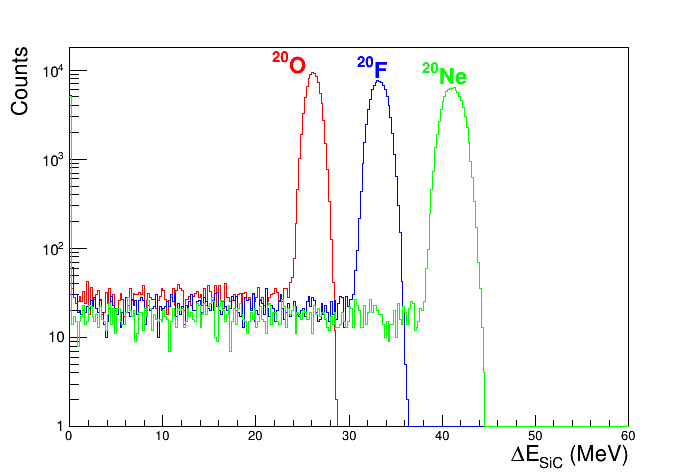
\includegraphics[scale=0.5]{Grafici_Tesi2/Particelle_non_ortogonali/deltaE.png}
%	\caption{Proiezione delle matrici di Figura~\ref{fig:fetta} sull'asse~$ E_{meas} $.} \label{fig:ETot1}
%\end{figure}


%\begin{figure} [!p]
%	\centering
%	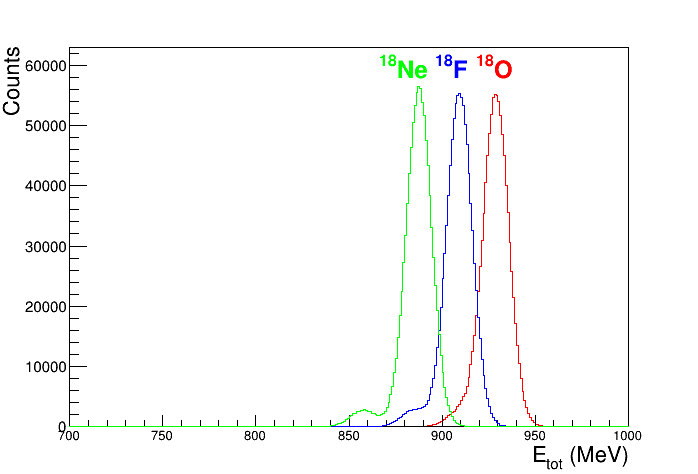
\includegraphics[scale=0.5]{Grafici_Tesi2/Particelle_non_ortogonali/ETot.png}
%	\caption{Proiezione delle matrici di Figura~\ref{fig:fetta} sull'asse~$ \Delta E_{SiC} $.} \label{fig:deltaE_Tot1}
%\end{figure}
%\begin{figure}[!p] 
%	\centering
%	\subfigure[]
%	{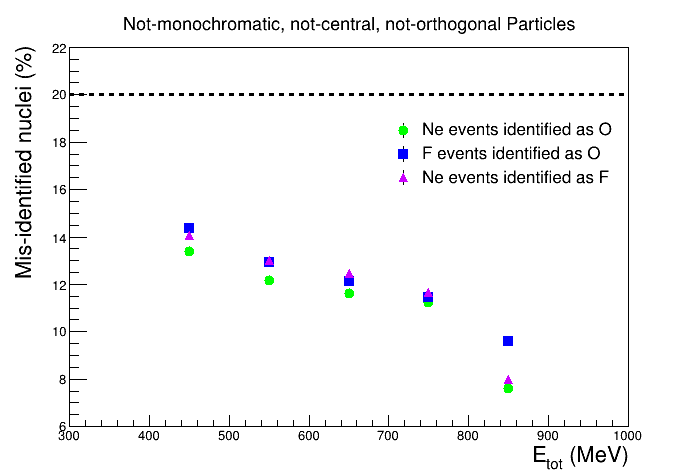
\includegraphics[scale=0.43]{Grafici_Tesi/Particelle_non_monocromatiche/leakage_alto_corr.png}}
%	\hspace{10mm}
%	\subfigure[]
%	{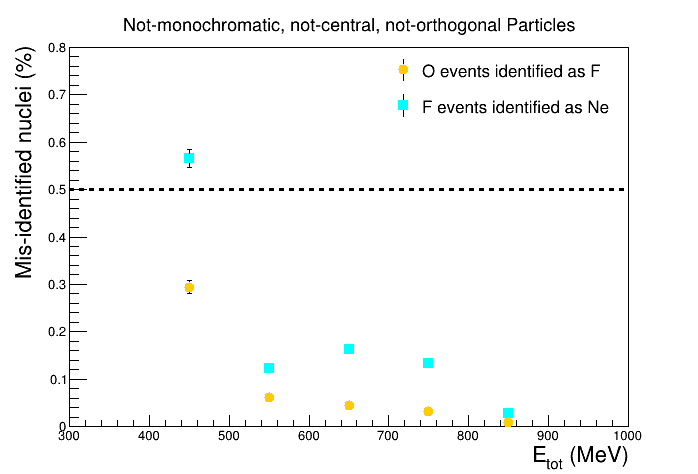
\includegraphics[scale=0.43]{Grafici_Tesi/Particelle_non_monocromatiche/leakage_basso_corr.png}}
%	\caption{La percentuale di nuclei identificati in modo erroneo in funzione di $E_{tot}$: in (a) la contaminazione da specie atomiche con $Z$ maggiore verso quelle con $Z$ minore, in (b) il viceversa. La linea tratteggiata in (a) indica il limite massimo imposto sul mancato riconoscimento del segnale, mentre in (b) rappresenta il limite massimo fissato sulla contaminazione del segnale. Laddove non sono mostrate, le barre di errore sono più piccole del marker.} \label{fig:leakage}
%\end{figure}

%\begin{figure} [!t]
%	\centering
%	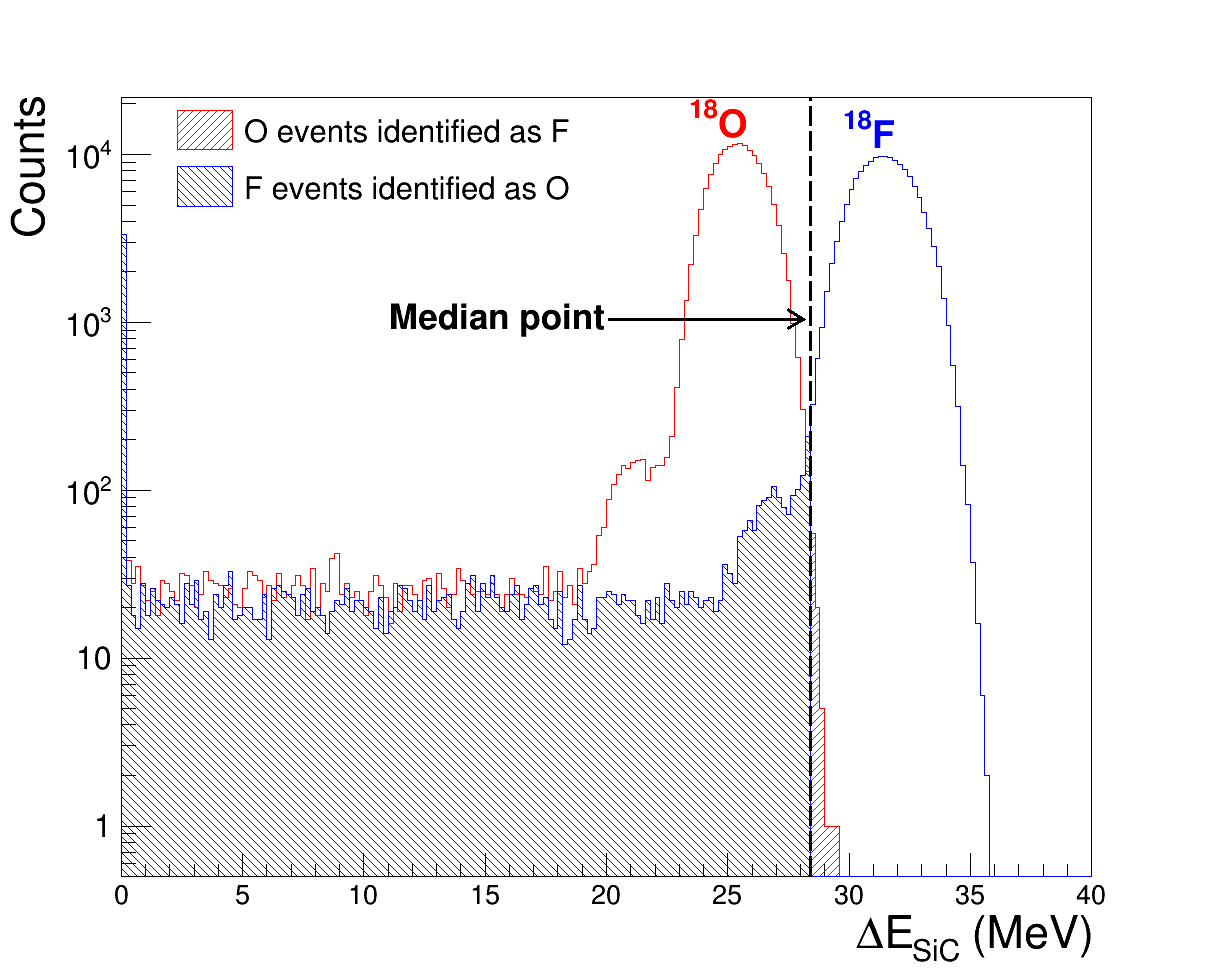
\includegraphics[scale=0.28]{Grafici_Tesi/Contaminazione/contaminazione.png}
%	\caption{Proiezione sull'asse $\Delta E_{SiC}$ della fetta in $E_{tot}$ compresa tra 600 e 700~MeV per l'\ce{^{18}O} e il \ce{^{18}F}. La linea tratteggiata indica il punto mediano tra i valori medi dei due spettri. In ombreggiatura blu si possono distinguere gli eventi di \ce{^{18}F} identificati come \ce{^{18}O}, in ombreggiatura rossa si notano gli eventi di \ce{^{18}O} identificati come \ce{^{18}F}.} \label{fig:fetta_con_contaminazione}
%\end{figure}










%%Allo scopo di dare una stima quantitativa della frazione di nuclei male identificati, si è proceduto nel modo seguente: si è diviso l'intero intervallo energetico $E_{tot}$ in un certo numero di fette; per ogni fetta si è effettuata una proiezione sull'asse $\Delta E_{SiC}$; per ogni coppia di specie atomiche si è calcolato il punto mediano fra i valori medi delle due distribuzioni; infine, si è determinato il numero di eventi al di sotto (o al di sopra) del punto mediano.
%%Un'immagine esemplificativa dell'idea alla base della procedura seguita è riportata in Figura~\ref{fig:fetta_con_contaminazione}: la linea tratteggiata indica il punto mediano tra i valori medi degli spettri di \ce{^{18}O} e \ce{^{18}F}.
%%A sinistra di tale punto sono evidenziati con ombreggiatura blu gli eventi di \ce{^{18}F} identificati come \ce{^{18}O}, mentre a destra sono contrassegnati con ombreggiatura rossa gli eventi di \ce{^{18}O} identificati come \ce{^{18}F}.
%%La contaminazione di \ce{^{18}F} in \ce{^{18}O} può essere, dunque, calcolata integrando lo spettro del \ce{^{18}F} da zero fino al punto mediano; invece, la contaminazione di \ce{^{18}O} in \ce{^{18}F} viene determinata integrando lo spettro dell'\ce{^{18}O} dal punto mediano fino alla fine della distribuzione.
%%La scelta del punto mediano come soglia è arbitraria e non necessariamente ottimale: è funzionale comunque per fare un confronto quantitativo e omogeneo fra molte configurazioni diverse.
%per quantificare la contaminazione di \ce{^{18}O} in \ce{^{18}F} si calcola 

%\begin{figure}[!p] 
%	\centering
%	\subfigure[]
%	{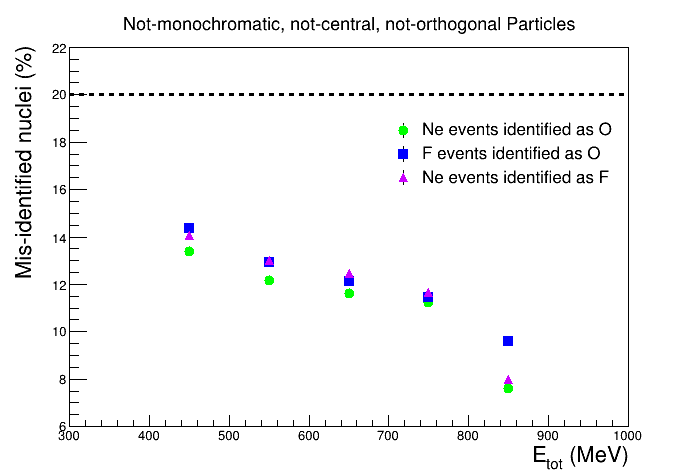
\includegraphics[scale=0.43]{Grafici_Tesi/Particelle_non_monocromatiche/leakage_alto_corr.png}}
%	\hspace{10mm}
%	\subfigure[]
%	{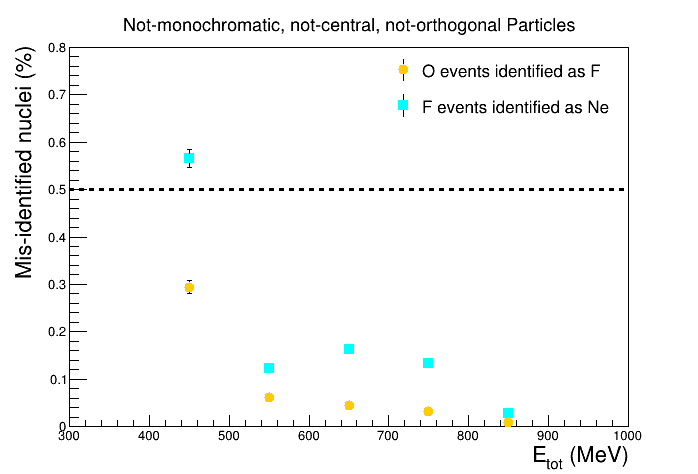
\includegraphics[scale=0.43]{Grafici_Tesi/Particelle_non_monocromatiche/leakage_basso_corr.png}}
%	\caption{La percentuale di nuclei identificati in modo erroneo in funzione di $E_{tot}$: in (a) la contaminazione da specie atomiche con $Z$ maggiore verso quelle con $Z$ minore, in (b) il viceversa. La linea tratteggiata in (a) indica il limite massimo imposto sul mancato riconoscimento del segnale, mentre in (b) rappresenta il limite massimo fissato sulla contaminazione del segnale. Laddove non sono mostrate, le barre di errore sono più piccole del marker.} \label{fig:leakage}
%\end{figure}


%%Il risultato di tale procedura è illustrato in Figura~\ref{fig:leakage}, dove il range energetico è stato suddiviso in intervalli da 100~MeV e si è scelto di rappresentare i dati soltanto laddove fossero presenti tutte e tre le bande.
%%Si può notare che la contaminazione da una specie atomica con $Z$ più grande verso una con $Z$ più piccolo è nettamente maggiore; infatti, le percentuali che si trovano in Figura~\ref{fig:leakage}.a sono comprese fra il 7\% e il 15\%, mentre quelle in Figura~\ref{fig:leakage}.b sono inferiori all'1\%.
%%In entrambi i casi si può osservare che la frazione di nuclei erroneamente identificati ha un andamento decrescente al crescere dell'energia.
%%Di conseguenza, a basse energie, dove gli effetti di raccolta parziale della carica sono maggiormente significativi, la capacità di separare gli ioni peggiora.
%%Infine, si può osservare che con la statistica simulata non si osserva una contaminazione di O in Ne, per cui si può mettere un limite superiore.







%%I due grafici in Figura~\ref{fig:leakage} sono estremamente importanti nella valutazione dell'idoneità di questo sistema di rivelazione agli scopi di NUMEN, in quanto per riuscire a misurare processi rari come quelli di DCE è essenziale che il segnale venga riconosciuto e che il fondo non venga identificato come segnale: se, ad esempio, consideriamo che il segnale da ricercare sia \ce{^{18}Ne}, allora gli eventi di tale ione identificati come \ce{^{18}O} o \ce{^{18}F} costituiscono una perdita di segnali corretti. 
%%Dunque, è necessario stabilire un limite inferiore alla probabilità di riconoscimento del segnale.
%%Ai fini di questo lavoro di tesi, tale limite può essere posto all'80\%.
%%D'altra parte, sempre considerando che il segnale sia costituito da \ce{^{18}Ne}, gli eventi di \ce{^{18}O} e \ce{^{18}F} identificati come \ce{^{18}Ne} rappresentano, invece, una contaminazione, ovvero fondo scambiato per segnale.
%%In questo caso bisogna fissare un limite superiore a tale contaminazione:
%%per gli scopi di questo lavoro, esso è stato posto allo 0.5\%.
%%Poiché gli eventi di fondo sono tipicamente molto più abbondanti di quelli di segnale, è necessario avere una selezione molto più stringente.
%%Questo evita che il numero di eventi di fondo erroneamente identificati come segnale sia comparabile con il numero dei reali eventi di segnale.

%(\textcolor{red}{Scrivere la parte sull'efficienza di riconoscimento del segnale})






%Uno studio interessante riguarda il confronto fra la correlazione $\Delta E_{SiC} - E_{tot}$ e quella $\Delta E_{SiC} - E_{CsI}$: in Figura~\ref{fig:deltaE_ERes}.
%%A questo punto, è interessante studiare la correlazione $\Delta E_{SiC} - E_{CsI}$: in Figura~\ref{fig:deltaE_ERes} sono riportate le matrici delle tre specie di interesse, le quali continuano ad essere ben separate per tutto il range energetico.
%%\begin{figure} [!p]
%	\centering
%	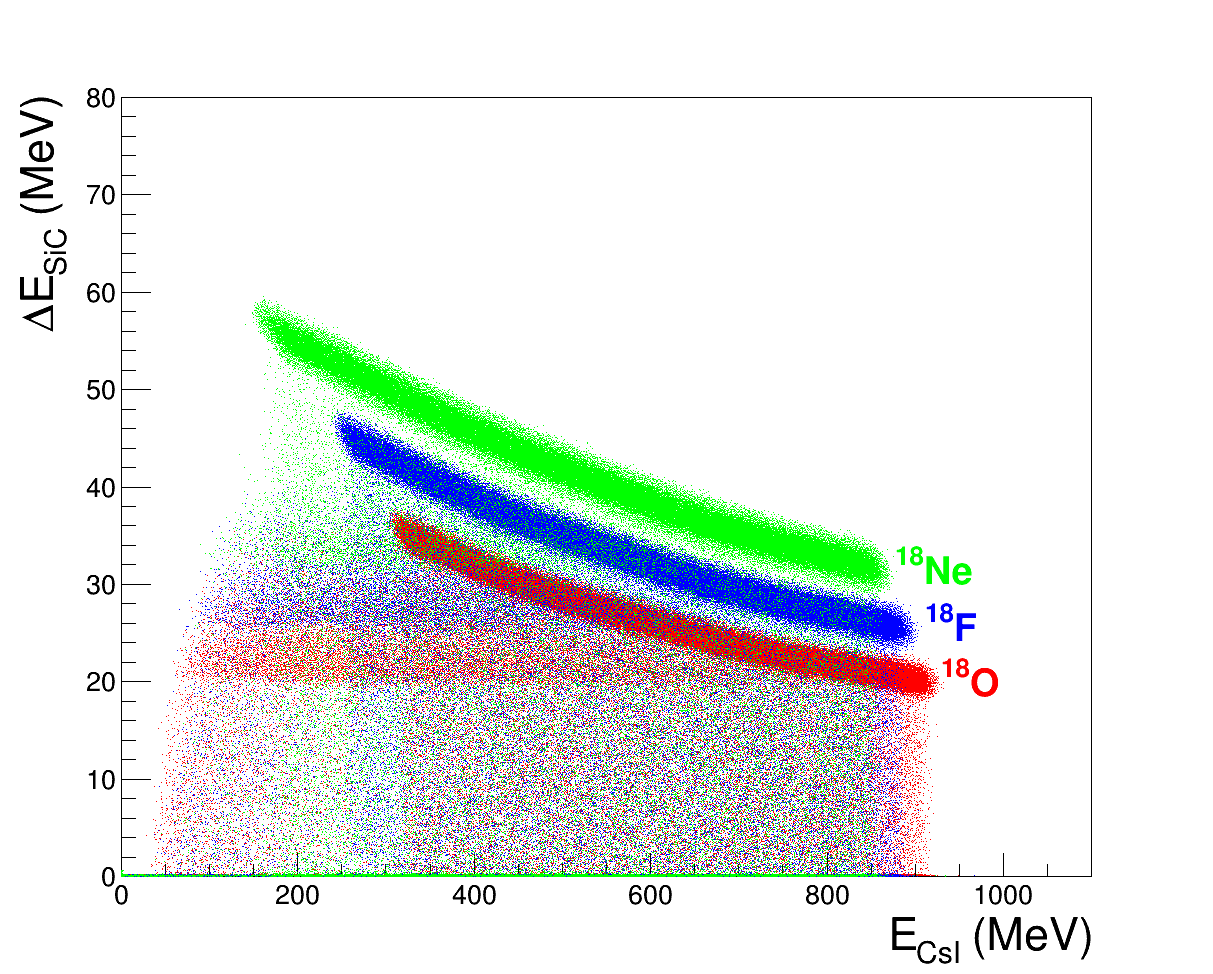
\includegraphics[width=\textwidth, keepaspectratio]{Grafici_Tesi/Particelle_non_monocromatiche_Resid/deltaE_ERes.png}
%	\caption{Matrici $\Delta E_{SiC} - E_{CsI}$.} \label{fig:deltaE_ERes}
%\end{figure} 
%Dal confronto con la Figura~\ref{fig:deltaE_ETot_full_energy} si nota che tali matrici si estendono ad energie inferiori, in quanto alla variabile sull'asse orizzontale viene a mancare il contributo di $\Delta E_{SiC}$. 
%%Confrontando tali matrici con quelle in Figura~\ref{fig:deltaE_ETot_full_energy}, non si notano sostanziali differenze, in particolare per quanto riguarda la densità degli eventi spuri.
%%Questa affermazione è supportata dalla Figura~\ref{fig:leakage_res}, nella quale si riscontrano percentuali simili a quelle viste in Figura~\ref{fig:leakage}.
%\begin{figure}[!p] 
%	\centering
%	\subfigure[]
%	{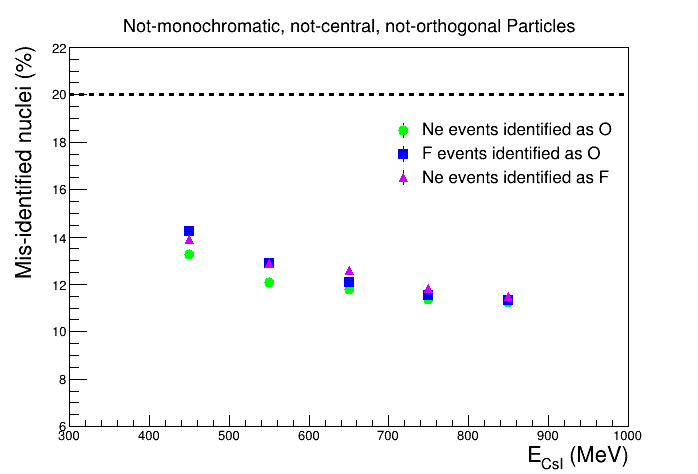
\includegraphics[scale=0.43]{Grafici_Tesi/Particelle_non_monocromatiche_Resid/leakage_alto_corr.png}}
%	\hspace{10mm}
%	\subfigure[]
%	{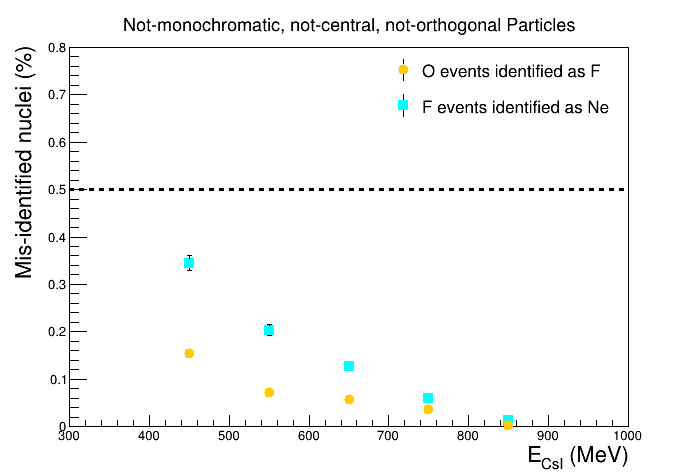
\includegraphics[scale=0.43]{Grafici_Tesi/Particelle_non_monocromatiche_Resid/leakage_basso_corr.png}}
%	\caption{La percentuale di nuclei identificati in modo erroneo in funzione di $E_{CsI}$: in (a) la contaminazione da specie atomiche con $Z$ maggiore verso quelle con $Z$ minore, in (b) il viceversa. La linea tratteggiata in (a) indica il limite massimo imposto sul mancato riconoscimento del segnale, mentre in (b) rappresenta il limite massimo fissato sulla contaminazione del segnale. Laddove non sono mostrate, le barre di errore sono più piccole del marker.} \label{fig:leakage_res}
%\end{figure}
%%L'unica differenza sembra essere dovuta al punto in Figura~\ref{fig:leakage_res}.a ad 850~MeV, per il quale si osservano percentuali lievemente maggiori del suo corrispettivo in Figura~\ref{fig:leakage}.a. 
%Ciò sembra essere legato al modo in cui si dispongono gli eventi con raccolta di carica incompleta; 
%%Ciò è legato alla correlazione delle due grandezze;
%%infatti, mentre nelle matrici $\Delta E_{SiC} - E_{tot}$ tali eventi scendono verso l'asse orizzontale con una certa inclinazione, nelle matrici $\Delta E_{SiC} - E_{CsI}$ la loro discesa verso all'asse $E_{CsI}$ procede in direzione perpendicolare. 
%%Sulla base di questo risultato è possibile sostenere che non è necessario effettuare una calibrazione energetica dei telescopi, in quanto ai fini della PID non vi è l'esigenza di sommare i valori di energia misurati dai due rivelatori.
%%Dal momento che il muro di telescopi sarà composto da oltre 1000 dispositivi, la possibilità di evitarne la calibrazione consentirebbe un notevole risparmio di tempo.
%Poiché la correlazione $\Delta E_{SiC} - E_{CsI}$ offre risultati paragonabili a quelli della correlazione $\Delta E_{SiC} - E_{tot}$, da questo momento in poi verranno presentate le matrici soltanto 











%%Poiché anche in altri casi si è riscontrato che la correlazione $\Delta E_{SiC} - E_{CsI}$ offre risultati paragonabili a quelli di $\Delta E_{SiC} - E_{tot}$, da questo momento in poi verranno presentate soltanto le matrici $\Delta E_{SiC} - E_{CsI}$.








%\vspace{0.5cm}
%\clearpage

\subsection{\iflanguage{italian}{Modello di interazioni adroniche}{Model with adronic interactions}} \label{par:interazioni_adroniche}

\begin{figure} [!p]
	\centering
	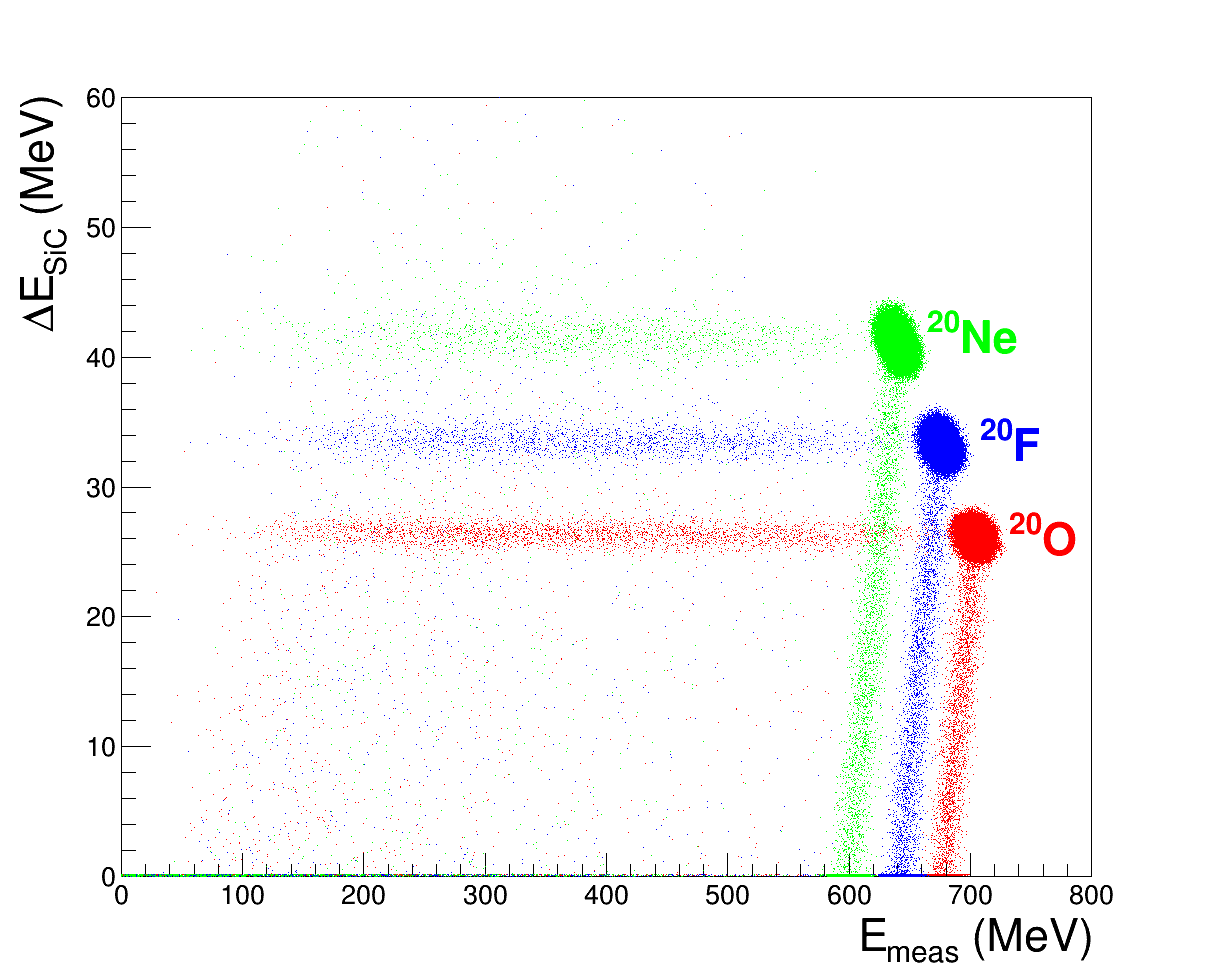
\includegraphics[width=\textwidth, keepaspectratio]{Grafici_Tesi2/Interazioni_adroniche/deltaE_ETot_quadrata.png}
	\caption{Le matrici $\Delta E_{SiC} - E_{meas}$ considerando un modello di processi fisici che comprenda anche le interazioni adroniche.} \label{fig:deltaE_ERes_adron}
\end{figure}





Rispetto all'esempio precedente, in questa simulazione la geometria e le caratteristiche delle particelle primarie restano invariate, mentre il modello dei processi fisici adesso include le interazioni adroniche. 
Le corrispondenti matrici $\Delta E_{SiC} - E_{meas}$ sono riportate in Figura~\ref{fig:deltaE_ERes_adron}: a differenza del caso in cui erano considerate soltanto le interazioni elettromagnetiche, si può osservare per tutte e tre le specie nucleari la comparsa di eventi ad un'energia $\Delta E_{SiC}$ più alta di quella dei rispettivi luoghi.
Ciò è dovuto a reazioni nucleari esotermiche, nelle quali viene rilasciata una quantità di energia aggiuntiva rispetto alla sola energia cinetica del proiettile.
%La presenza di questi eventi non sembra provocare significativi cambiamenti nelle capacità di PID, in quanto, come si può evincere dalla Figura~\ref{fig:leakage_res_adron}, le percentuali di nuclei potenzialmente male identificati aumentano di meno dell'1\%.
%L'unico mutamento degno di nota riguarda la comparsa di contaminazioni di O in Ne.
%Dunque, è evidente che la maggior parte degli eventi spuri è originata da raccolta di carica incompleta, come d'altronde era lecito aspettarsi vista la minore probabilità che avvenga un'interazione adronica.






%\begin{figure}[!p] 
%	\centering
%	\subfigure[]
%	{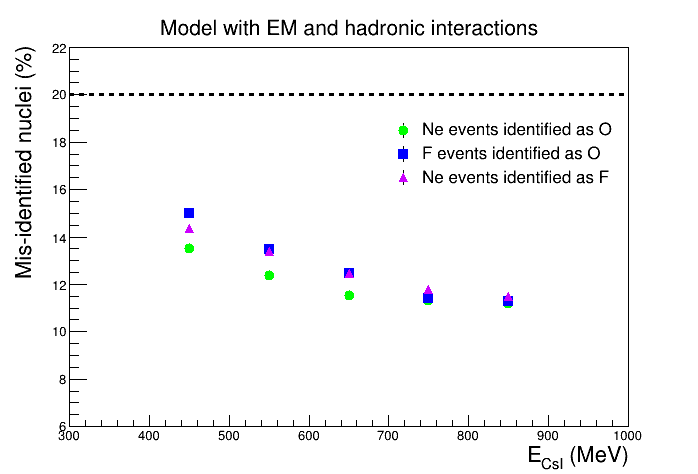
\includegraphics[scale=0.43]{Grafici_Tesi/Interazioni_adroniche/leakage_alto_corr.png}}
%	\hspace{10mm}
%	\subfigure[]
%	{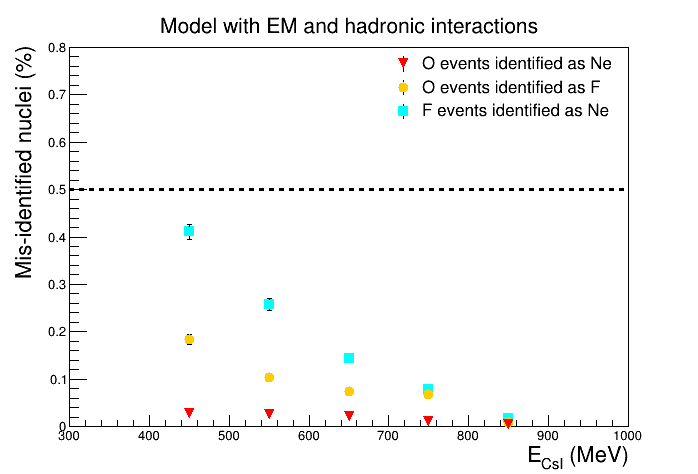
\includegraphics[scale=0.43]{Grafici_Tesi/Interazioni_adroniche/leakage_basso_corr.png}}
%	\caption{La percentuale di nuclei identificati in modo erroneo in funzione di $E_{CsI}$, utilizzando un modello che comprenda anche le interazioni adroniche: in~(a) la contaminazione da specie atomiche con $Z$ maggiore verso quelle con $Z$ minore, in (b) il viceversa. La linea tratteggiata in (a) indica il limite massimo imposto sul mancato riconoscimento del segnale, mentre in (b) rappresenta il limite massimo fissato sulla contaminazione del segnale. Laddove non sono mostrate, le barre di errore sono più piccole del marker.} \label{fig:leakage_res_adron}
%\end{figure}


%\clearpage

\subsection{\iflanguage{italian}{Studio delle capacità di PID}{Study of PID performance}} \label{sez:studio_PID}

%Uno degli obiettivi fondamentali di questo lavoro di tesi consiste nel valutare la risposta del telescopio SiC-CsI agli eventi  

Dopo aver esposto tre casi ideali, utili per comprendere alcuni fenomeni rilevanti incontrati in questo studio, si esamina adesso una situazione realistica, in cui alla simulazione \geant{} viene dato in input il file prodotto dai software per il trasporto degli eiettili attraverso MAGNEX.
In questo caso, dunque, gli ioni presentano sia le correlazioni cinematiche sia quelle legate alle proprietà ottiche dello spettrometro.
A differenza dei casi precedenti, sono stati simulati sette milioni di eventi ugualmente distribuiti su sette tipi di ioni, ossia \ce{^{20}O^{8+}}, \ce{^{21}O^{8+}}, \ce{^{20}F^{8+}}, \ce{^{21}F^{8+}}, \ce{^{20}Ne^{8+}}, \ce{^{21}Ne^{8+}} e \ce{^{22}Ne^{8+}}.
Mentre il primo rappresenta lo ione di interesse, gli altri sono le principali sorgenti di contaminazione quando si studia una reazione di DCE in cui l'\ce{^{20}O^{8+}} è nel suo stato fondamentale.
Altri ioni, come ad esempio il \ce{^{19}F^{8+}} e l'\ce{^{19}O^{8+}}, e altri stati di carica, per esempio i $9^+$ e i $10^+$, non sono stati presi in considerazione perché, per ragioni cinematiche e per le proprietà ottiche dello spettrometro, vengono rivelati in regioni del FPD lontane da quella in cui arriva lo ione di interesse.
Il telescopio ha dimensioni trasversali di 1.5~cm $\times$ 1.5~cm ed è posto a 14~cm di distanza dal piano in cui vengono prodotte le particelle primarie, che coincide con il piano di ingresso nel FDP.



%Per fissare la rigidità magnetica di riferimento si è scelto il \ce{^{18}Ne^{10+}}, che fra gli ioni considerati è quello con il rapporto massa su carica più piccolo.
La rigidità magnetica di riferimento è stata scelta in modo che l'\ce{^{20}O^{8+}} nel suo stato fondamentale fosse focalizzato al centro del FPD, ovvero in corrispondenza del telescopio.
%Gli altri ioni, dal momento che hanno un rapporto massa su carica uguale o molto vicino a quello dell'\ce{^{20}O^{8+}}, 
%Si fa notare che, dovendo mantenere costante il prodotto $\sqrt{m}/q \cdot \sqrt{E}$, gli altri ioni hanno energia cinetica inferiore.
Dovendo tutti gli ioni simulati avere la stessa finestra di rigidità magnetica, all'aumentare del rapporto $\sqrt{m}/q$, l'energia cinetica $E$ deve diminuire.
Questa considerazione è confermata dalla Figura~\ref{fig:KinE}, in cui viene illustrato lo spettro delle energie cinetiche di \ce{^{20}Ne^{8+}}, \ce{^{21}Ne^{8+}} e \ce{^{22}Ne^{8+}}.
\begin{figure} [!p]
	\centering
	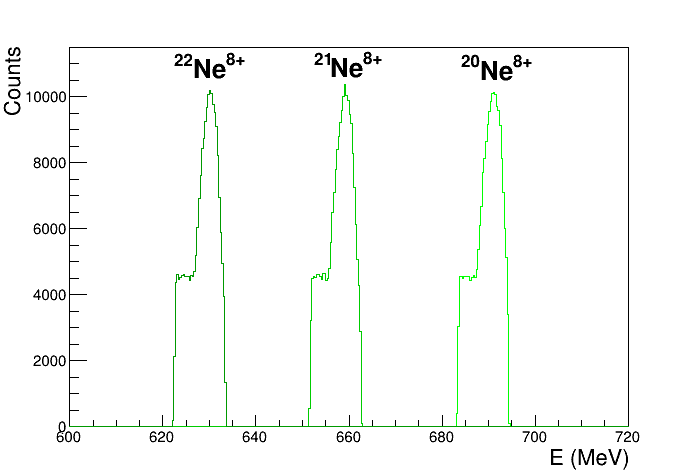
\includegraphics[width=\textwidth, keepaspectratio]{Grafici_Tesi2/PIDnew/ekin.png}
	\caption{Lo spettro delle energie cinetiche~$E$ per \ce{^{20}Ne^{8+}}, \ce{^{21}Ne^{8+}} e \ce{^{22}Ne^{8+}}.} \label{fig:KinE}
\end{figure}
Per lo stesso motivo, ioni che hanno lo stesso rapporto massa su carica devono avere lo stesso intervallo di energia cinetica, per cui, ad esempio, la finestra di $E$ dell'\ce{^{20}O^{8+}} coincide con quella del \ce{^{20}Ne^{8+}}.
Come si può notare, per ogni ione il range energetico che arriva sul telescopio è di circa 9~MeV, in buon accordo con la~\ref{eq:finestra_Brho}.
%Da tale figura si evince che le energie cinetiche accettate dal telescopio sono molto differenti per i diversi ioni, con una differenza fra lo ione più energetico e quello meno energetico di oltre 350~MeV.
%La Figura~\ref{fig:KinE}.b mostra un ingrandimento della precedente nella zona degli ioni di ossigeno: come si può notare, per ogni ione il range energetico che arriva sul telescopio è di circa 8~MeV, in buon accordo con la~\ref{eq:finestra_Brho}.
%Gli ioni hanno la stessa finestra di rigidità magnetica, per cui tutti vanno a finire sul telescopio simulato. 


%\begin{figure} [!p]
%	\centering
%	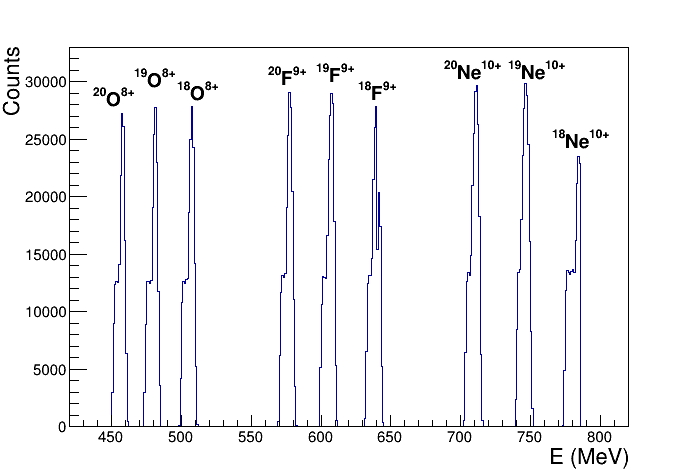
\includegraphics[scale=0.4]{Grafici_Tesi2/PID/KinE2.png}
%	\caption{Lo spettro delle energie cinetiche~$E$ dei diversi ioni simulati.} \label{fig:KinE}
%\end{figure}

%\begin{figure} [!p]
%	\centering
%	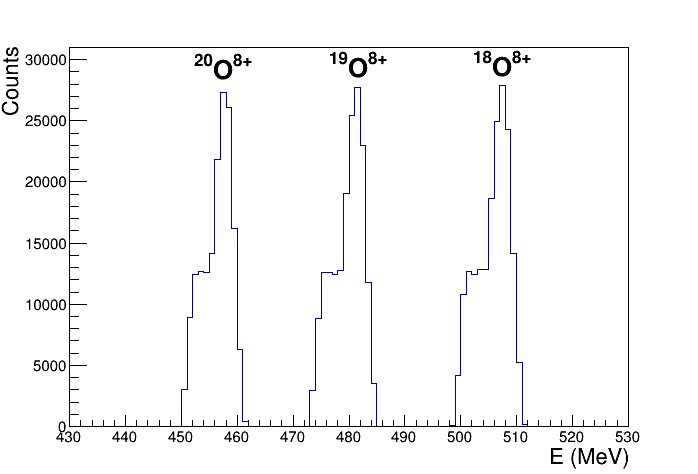
\includegraphics[scale=0.4]{Grafici_Tesi2/PID/KinE_zoom.png}
%	\caption{Ingrandimento della spettro in Figura~\ref{fig:KinE} nella zone degli ioni di ossigeno.} \label{fig:KinE_zoom}
%\end{figure}





Le corrispondenti matrici $\Delta E_{SiC} - E_{meas}$ sono riportate in Figura~\ref{fig:deltaE_Emeas_PID}: come si può notare, i luoghi degli ioni simulati appaiono ben separati sia in numero atomico~($Z$) sia in numero di massa~($A$).
\begin{figure} [!p]
	\centering
	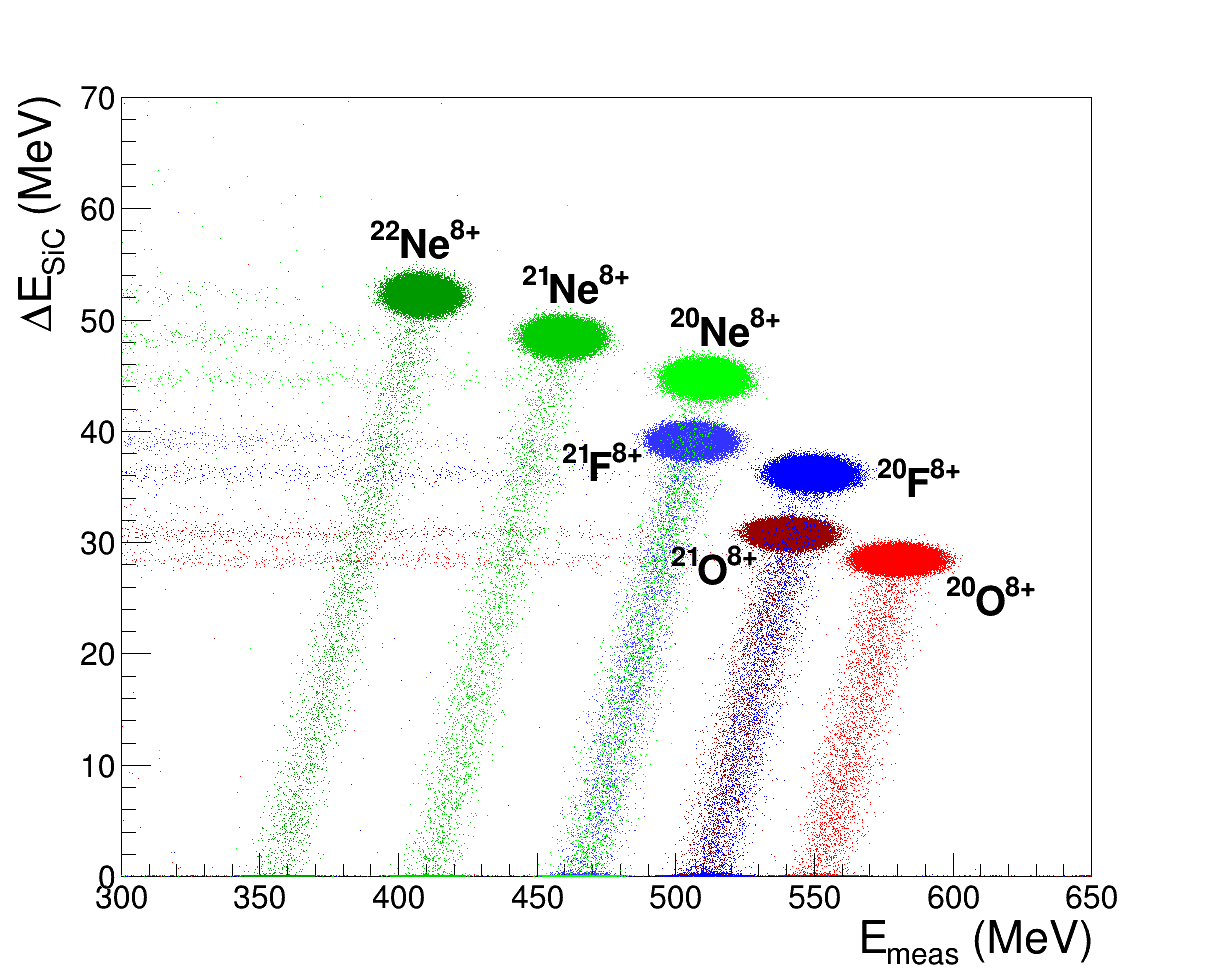
\includegraphics[width=\textwidth, keepaspectratio]{Grafici_Tesi2/PIDnew/deltaE_Emeas_quadrata_menoeventi2.png}
	\caption{Le matrici $\Delta E_{SiC} - E_{meas}$ considerando per tutti gli ioni sia la cinematica di reazione sia il trasporto ottico.} \label{fig:deltaE_Emeas_PID}
\end{figure}
%Si può, inoltre, osservare che l'energia rilasciata nel rivelatore al~SiC è molto simile per le tre specie atomiche: 
%ciò dipende dalla notevole differenza in energia cinetica degli ioni che compensa la variazione legata al cambiamento di $Z$.
%ciò dipende dal fatto che, a causa del filtro in $B \rho$, gli ioni con carica $q$ più piccola hanno energia cinetica minore, mentre quelli con $q$ più grande hanno energia cinetica maggiore; ricordando che nella formula di Bethe-Bloch la perdita di energia è proporzionale a $Z^2$ e inversamente proporzionale ad $E$, si può dedurre che la notevole differenza in energia cinetica degli ioni compensa la variazione legata al cambiamento di $Z$.
%Di conseguenza, assumendo di essere interessati ad una reazione di DCE in cui si vuole rivelare l'\ce{^{20}O}, la principale componente di contaminazione nell'identificazione proviene dagli ioni che non si fermano nel rivelatore al~CsI.
%Di conseguenza, nel caso in esame la principale componente di contaminazione nell'identificazione degli eventi di interesse proviene dagli ioni che non si fermano nel rivelatore al~CsI.
%Di conseguenza, nel caso in esame la principale componente di contaminazione nella PID proviene dagli ioni che non si fermano nel rivelatore al~CsI.
Si può, inoltre, osservare che anche in questo caso sono presenti sia gli eventi degradati dovuti alla parziale raccolta della carica nel rivelatore al~SiC, sia quelli originati dall'incompleto rilascio dell'energia residua nel cristallo di~CsI.
Alla significativa separazione in $E_{meas}$ delle matrici contribuisce il substrato passivato del rivelatore al~SiC, nel quale ioni con $Z$ diverso perdono quantità di energie notevolmente differenti.
Per dare una stima quantitativa della percentuale degli eventi degradati, che potrebbero costituire un fondo nella regione di interesse (Region Of Interest, ROI), si è proceduto nel modo seguente: supponendo di voler analizzare una reazione di DCE in cui si vuole rivelare l'\ce{^{20}O^{8+}} nello stato fondamentale, si è effettuato nel plot $\Delta E_{SiC} - E_{meas}$ un taglio grafico attorno al luogo pertinente a tale ione, come mostrato in Figura~\ref{fig:deltaE_Emeas_taglio}.
\begin{figure} [!p]
	\centering
	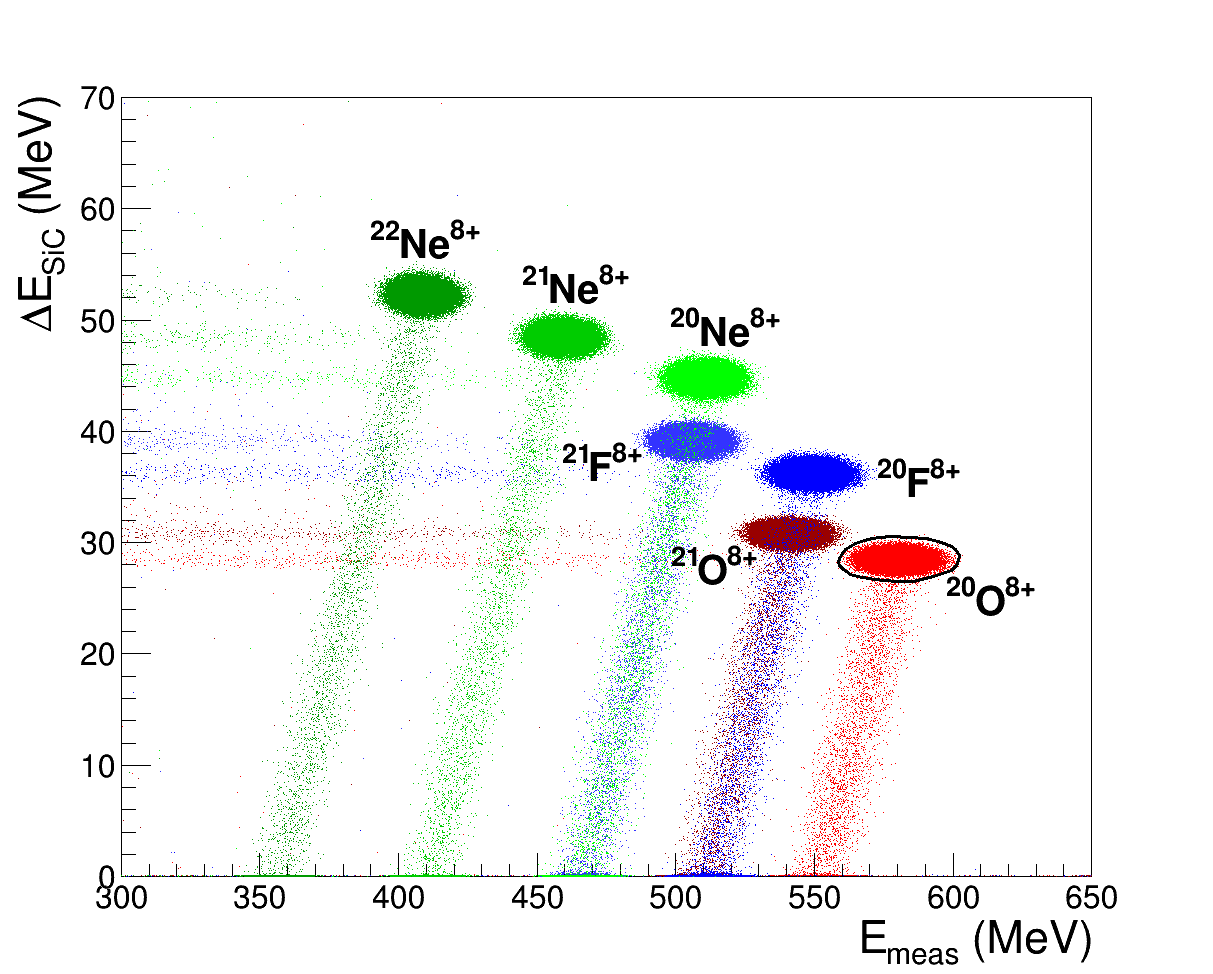
\includegraphics[width=\textwidth, keepaspectratio]{Grafici_Tesi2/PIDnew/deltaE_Emeas_quadrata_taglio_menoeventi2.png}
	\caption{Taglio grafico per l'identificazione dell'\ce{^{20}O^{8+}} e per il calcolo delle percentuali di contaminazione.} \label{fig:deltaE_Emeas_taglio}
\end{figure}
All'interno del taglio sono presenti, oltre allo ione di interesse, anche altre specie ioniche, che potrebbero essere erroneamente identificate come~\ce{^{20}O^{8+}}.
La percentuale di contaminazione nella ROI dovuta ad un particolare ione può essere calcolata dividendo il numero di eventi di quello ione presenti nella ROI per il numero totale di eventi dello stesso.
%Supponiamo, adesso, di essere interessati ad una reazione di DCE in cui si vuole rivelare l'\ce{^{20}O}: il primo passo nell'analisi dei dati consiste nell'identificazione degli ioni di interesse attraverso l'utilizzo di tagli grafici.
Il risultato di tale operazione, nel caso del taglio grafico considerato in Figura~\ref{fig:deltaE_Emeas_taglio}, è riportato in Tabella~\ref{tab:contaminazione_deltaE_Emeas_1.5per1.5}: come si può notare, le percentuali sono molto basse, a dimostrazione delle grandi capacità di PID del telescopio~SiC-CsI.
Per gli ioni per i quali non è stata riscontrata contaminazione nella ROI si è assunto che il numero di eventi in tale regione fosse minore di 2.3 al 90\% di livello di confidenza (Confidence Level, CL).
\begin{table} [t!]
	\begin{center}
		\renewcommand{\arraystretch}{1.2}
		\begin{tabular} {cccc}
			Ione               & & &   Contaminazione nella ROI (\%) \\
			\toprule[0.1em]
			%\hline
			\ce{^{21}O^{8+}}   & & &   0.003 $\pm$ 0.001 \\
			\hline
			\ce{^{20}F^{8+}}   & & &   0.0005 $\pm$ 0.0005 \\
			\hline
			\ce{^{21}F^{8+}}   & & &  < 0.0011 al 90\% CL \\
			\hline
			\ce{^{20}Ne^{8+}}   & & &  < 0.0011 al 90\% CL \\
			\hline
			\ce{^{21}Ne^{8+}}   & & &  < 0.0011 al 90\% CL \\
			\hline
			\ce{^{22}Ne^{8+}} & & &   < 0.0011 al 90\% CL\\
			\bottomrule[0.1em]
		\end{tabular}
	\end{center}
	\caption{La contaminazione dei diversi ioni nella ROI dell'\ce{^{20}O^{8+}} individuata dal taglio grafico in Figura~\ref{fig:deltaE_Emeas_taglio}.} \label{tab:contaminazione_deltaE_Emeas_1.5per1.5}
\end{table}
%La contaminazione più rilevante deriva dall'\ce{^{21}O^{8+}}, come era lecito aspettarsi considerando che si tratta della specie ionica che hanno un valore di $\Delta E_{SiC}$ molto simile a quello dell'\ce{^{20}O^{8+}}.
%La percentuale di eventi di~\ce{^{20}O^{8+}} persi nell'identificazione può essere determinata dividendo il numero di eventi di~\ce{^{20}O^{8+}} al di fuori della ROI per il numero totale di eventi dello stesso: dal calcolo risulta che tale percentuale è del~$(9.14 \pm 0.08)$~\%.
L'efficienza di rivelazione del segnale può essere determinata dividendo il numero di eventi di~\ce{^{20}O^{8+}} nella ROI per il numero totale di eventi dello stesso; dal calcolo risulta che essa è pari al $(90.4 \pm 0.2)$~\%.
La restante parte del segnale viene persa a causa dell'incompleta raccolta di carica nel rivelatore al~SiC o del parziale rilascio dell'energia residua nel cristallo di~CsI.






%A questo punto è bene sottolineare che finora le contaminazioni sono state calcolate simulando per tutti gli ioni lo stesso numero di eventi.
%Tuttavia, nella situazione reale la produzione degli ioni considerati avviene attraverso meccanismi di reazioni nucleari, ciascuno caratterizzato da una certa sezione d'urto; questa rappresenta, infatti, la probabilità con cui può verificarsi una determinata reazione.  
A questo punto è bene sottolineare che finora le contaminazioni sono state calcolate senza tenere in considerazione che nella situazione reale la produzione degli ioni avviene attraverso meccanismi di reazioni nucleari, ciascuno caratterizzato da una certa sezione d'urto; questa rappresenta, infatti, la probabilità con cui può verificarsi una determinata reazione.
I valori tipici delle sezioni d'urto sperimentali dei processi coinvolti in questa simulazione, normalizzati alla sezione d'urto sperimentale peculiare del DCE, sono riportati nella Tabella~\ref{tab:sez_d'urto}, insieme alla probabilità di avere uno ione in un certo stato di carica dopo il passaggio attraverso un foglio di carbonio.
È bene precisare che, per l'\ce{^{19}O}, il valore indicato non deriva da misure sperimentali ma da considerazioni sull'ordine del processo stesso.
\begin{table} [p!]
	\begin{center}
		\renewcommand{\arraystretch}{1.2}
		\begin{tabular} {cccccccl}
			Reazione & & Ione & & Sez. d'urto sperim.  & & \multicolumn{2}{c}{Fraz. di stato di carica}  \\
			& &      & &    norm. al DCE    & &&                          \\
			\toprule[0.1em]
			%\hline
			DCE        & & \ce{^{20}O}  & &        1        & & & $8^+ \sim 0.9963$ \\
			\hline
			SCE        & & \ce{^{20}F}  & &     $10^4$      & & & $9^+ \sim 0.99934$ \\
			& &              & &                 & & & $8^+ \sim 6.6 \cdot 10^{-4}$ \\
			\hline
			1-neutron  & & \ce{^{21}Ne} & &  $3\cdot10^4 $  & & & $10^+ \sim 0.99905$ \\
			& &              & &                 & & & $9^+ \sim 10^{-5}$ \\
			& &              & &                 & & & $8^+ \sim 10^{-7}$ \\
			\hline
			2-neutron  & & \ce{^{22}Ne} & &     $10^2 $     & & & $10^+ \sim 0.99905$ \\
			& &              & &                 & & & $9^+ \sim 10^{-5}$ \\
			& &              & &                 & & & $8^+ \sim 10^{-7}$ \\
			\hline
			inelastic  & & \ce{^{20}Ne} & &     $10^4 $     & & & $10^+ \sim 0.99905$ \\
			& &              & &                 & & & $9^+ \sim 10^{-5}$ \\
			& &              & &                 & & & $8^+ \sim 10^{-7}$ \\
			\hline
			$3^{\mbox{rd}}$ order multi- & & \ce{^{21}F}  & &     $10^3 $     & & & $9^+ \sim 0.99934$ \\
			nucleon transfer      & &              & &                 & & & $8^+ \sim 6.6 \cdot 10^{-4}$ \\
			\hline
			$5^{\mbox{th}}$ order multi-   & & \ce{^{19}O}  & &        0.1       & & & $8^+ \sim 0.99963$ \\
			nucleon transfer              & &              & &                 & & &  \\
			
			\bottomrule[0.1em]
		\end{tabular}
		
	\end{center}
	\caption{I valori tipici delle sezioni d'urto sperimentali di diversi processi di reazioni nucleari normalizzate alla sezione d'urto del DCE. Si riporta, inoltre, la probabilità di avere uno ione in un determinato stato di carica dopo aver attraversato un foglio di carbonio. Si sottolinea che, nel caso dell'\ce{^{19}O}, il valore della sezione d'urto indicato non deriva da misure sperimentali ma da considerazioni sull'ordine del processo stesso.} \label{tab:sez_d'urto}
\end{table}
Moltiplicando il valore della sezione d'urto sperimentale tipica di un processo per la probabilità di ottenere uno stato di carica, si può determinare la probabilità di produrre, a seguito di una reazione nucleare, uno ione in un determinato stato di carica;
%%Moltiplicando i numeri della terza colonna con quelli della quarta, si può determinare la probabilità di ottenere, a seguito di una reazione nucleare, uno ione in un determinato stato di carica.
questo è il fattore con cui bisogna riscalare le percentuali precedentemente mostrate per stimare le contaminazioni reali.
Il risultato di questa operazione è riportato in Tabella~\ref{tab:contaminazioni_riscalate}: come si può osservare, il contributo maggiore deriva dal SCE (\ce{^{20}F}).

\begin{table} [t!]
	\begin{center}
		\renewcommand{\arraystretch}{1.2}
		\begin{tabular} {cccc}
			Ione &  Stato di carica & & Numero di eventi nella ROI  \\
			&                  & &   norm. ad 1 evento di DCE  \\
			\toprule[0.1em]
			%\hline
			\ce{^{20}O}    &  $8^+$   & &  $0.904 \pm 0.002$      \\
			\hline
			\ce{^{21}O}    &  $8^+$   & &  $\sim 3 \cdot 10^{-6}$      \\
			\hline
			\ce{^{20}F}    &  $8^+$   & &  $\sim 3 \cdot 10^{-5}$       \\
			\hline
			\ce{^{21}F}    &  $8^+$   & &  $< 10^{-7} $ al 90\% CL     \\
			\hline
			\ce{^{20}Ne}    &  $8^+$   & &  $< 10^{-8}$ al 90\% CL        \\
			\hline
			\ce{^{21}Ne}   &  $8^+$  & &  $< 10^{-7} $  al 90\% CL    \\
			\hline
			\ce{^{22}Ne}   &  $8^+$  & &  $< 10^{-9}$    al 90\% CL    \\
			\bottomrule[0.1em]
		\end{tabular}
	\end{center}
	\caption{Per ogni ione si riporta il numero di eventi nella ROI normalizzato ad un evento di segnale.} \label{tab:contaminazioni_riscalate}
\end{table}

Dividendo il numero di segnali per la somma degli eventi di fondo, si ottiene una quantità nota come \emph{rapporto segnale-background}~(S/B), che in questo caso risulta essere di $24174 \pm 62$.
A partire da questo valore è possibile risalire alla sensibilità di misura nel modo seguente: sapendo che la sezione d'urto tipica del DCE nel range di energia di eccitazione studiato è di circa 1000~nb, dal rapporto S/B si deduce che il fondo corrisponde a circa 40~pb ad 1$\sigma$ di errore; dunque, considerando 5$\sigma$, si trova una sensibilità di circa 200~pb.
Mentre il fondo ha una sezione d'urto circa costante, quella del DCE ha una forte dipendenza dall'energia; in particolare, nella regione di interesse, che arriva fino ad 1~MeV di energia di eccitazione, la sezione d'urto del DCE è di circa 10~nb.
Pertanto, con la sensibilità di misura stimata, l'apparato sperimentale sarebbe in grado di misurare la reazione di interesse.







\subsection*{\iflanguage{italian}{Studio della correlazione $\Delta E_{SiC} - E_{CsI}$}{Study of $\Delta E_{SiC} - E_{CsI}$ correlation}}




Un aspetto importante di questo studio consiste nel valutare se la correlazione $\Delta E_{SiC} - E_{CsI}$ possa dare risultati analoghi a quelli ottenuti con la correlazione $\Delta E_{SiC} - E_{meas}$. 
%In Figura~\ref{fig:deltaE_Ecsi} si riportano le matrici degli ioni completamente ionizzati, le quali continuano ad essere ben separate.
%Le percentuali di contaminazione nella ROI individuata dal taglio grafico in figura sono mostrate nella Tabella~\ref{tab:contaminazione_deltaE_Ecsi_1.5per1.5}; confrontando quest'ultima con la Tabella~\ref{tab:contaminazione_deltaE_Emeas_1.5per1.5} si può osservare che le percentuali sono molto simili.
%Lo stesso risultato si ottiene considerando gli ioni con stati di carica diversi, le cui matrici sono rappresentate in Figura~\ref{fig:deltaE_Ecsi_stati_carica}.
%Anche le matrici degli ioni non completamente ionizzati restano chiaramente distinte, come si può osservare dalla Figura~\ref{fig:deltaE_Ecsi_stati_carica}.  
In Figura~\ref{fig:deltaE_Ecsi} sono riportate le matrici degli ioni simulati: come si può notare, anche in questo caso esse sono ben separate sia in numero atomico sia in numero di massa.
\begin{figure} [!p]
	\centering
	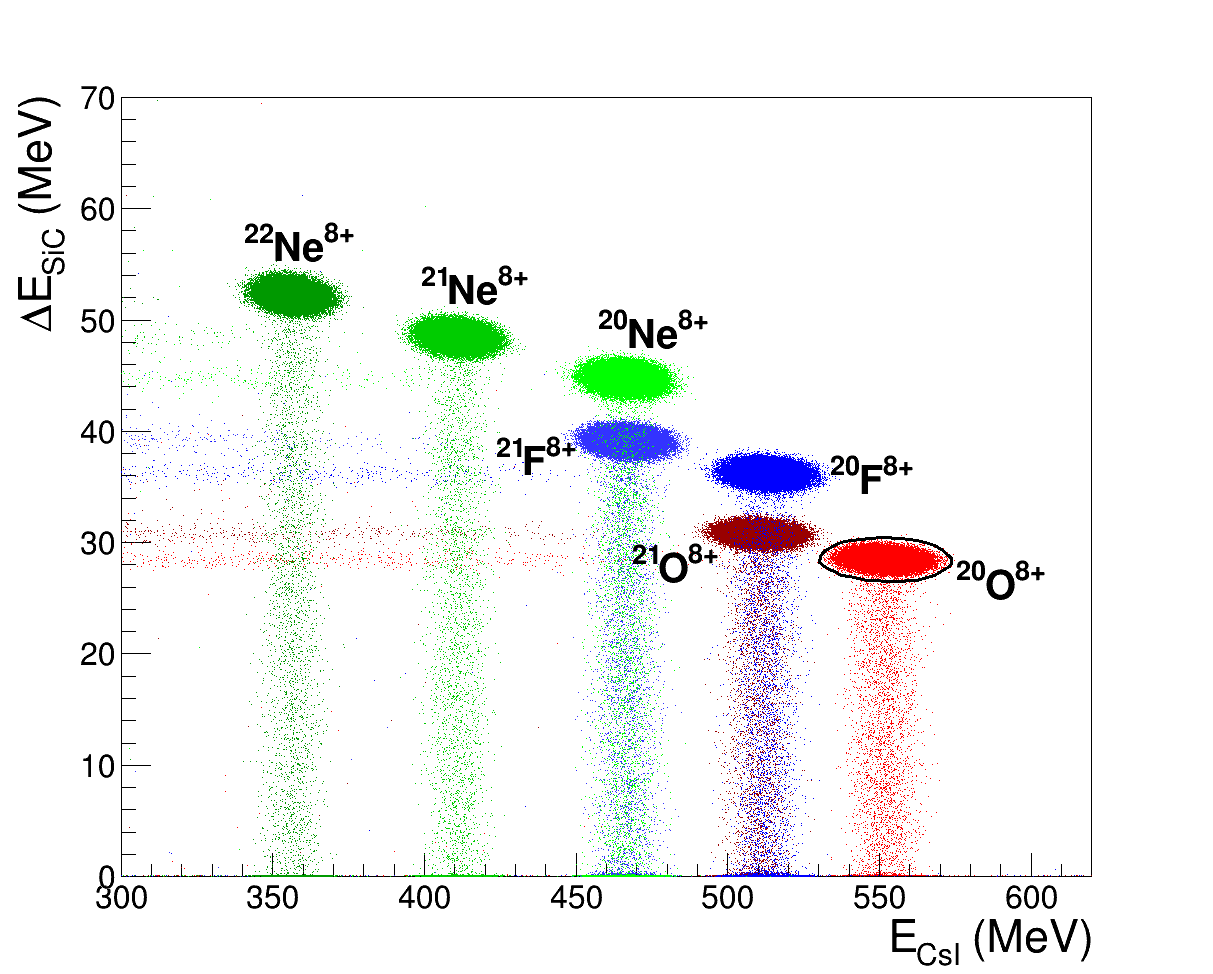
\includegraphics[width=\textwidth, keepaspectratio]{Grafici_Tesi2/PIDnew/deltaE_Ecsi_quadrata_taglio_menoeventi2.png}
	\caption{Le matrici $\Delta E_{SiC} - E_{CsI}$. Viene, inoltre, mostrato il taglio grafico per l'identificazione dell'\ce{^{20}O^{8+}} e per il calcolo delle percentuali di contaminazione.} \label{fig:deltaE_Ecsi}
\end{figure}
Il numero di eventi nella ROI, riscalato per la sezione d'urto e per la probabilità di ottenere un certo stato di carica e normalizzato ad un evento di DCE, è mostrato in Tabella~\ref{tab:contaminazioni_deltaE_Ecsi_riscalate}: confrontando quest'ultima con la Tabella~\ref{tab:contaminazioni_riscalate} si può osservare che i valori sono, per tutti gli ioni considerati, molto simili.
L'efficienza di rivelazione del segnale resta del $(90.4 \pm 0.2)$~\%, mentre il rapporto S/B risulta essere pari a $10939 \pm 28 $, inferiore a quello trovato con la correlazione $\Delta E_{SiC} - E_{meas}$.
La sensibilità di misura corrispondente a questo valore è di circa 460~pb a 5$\sigma$, pertanto anche con questo tipo di correlazione è possibile misurare le reazioni di DCE all'energia di eccitazione di interesse.
Sulla base di queste considerazioni è possibile sostenere che non è necessario effettuare una calibrazione energetica dei telescopi, in quanto ai fini della PID non vi è l'esigenza di sommare i valori di energia misurati dai due rivelatori. 
Dal momento che il muro di telescopi sarà composto da oltre 1200 dispositivi, la possibilità di evitarne la calibrazione consentirebbe un notevole risparmio di tempo necessario per la riduzione dei dati.
Poiché la correlazione $\Delta E_{SiC} - E_{CsI}$ ha dimostrato offrire una sensibilità di misurare adatta agli scopi del progetto, da questo momento in poi verranno presentate soltanto le matrici relative a questa correlazione.
%Poiché il rapporto S/B ottenuto dalla correlazione $\Delta E_{SiC} - E_{CsI}$ si è dimostrato superiore a quello della correlazione $\Delta E_{SiC} - E_{meas}$, da questo momento in poi verranno presentate soltanto le matrici relative a

%\begin{table} [t!]
%	\begin{center}
%		\renewcommand{\arraystretch}{1.2}
%		\begin{tabular} {cccc}
%			Ione               & & &   Contaminazione nella ROI (\%) \\
%			\toprule[0.1em]
%			%\hline
%			\ce{^{18}O^{8+}}   & & &   0.0011 $\pm$ 0.0008 \\
%			\ce{^{19}O^{8+}}   & & &   0.006 $\pm$ 0.0006 \\
%			\ce{^{18}F^{9+}}   & & &   0.013 $\pm$ 0.003 \\
%			\ce{^{19}F^{9+}}   & & &   0.082 $\pm$ 0.006 \\
%			\ce{^{20}F^{9+}}   & & &   0.042 $\pm$ 0.005 \\
%			\ce{^{18}Ne^{10+}} & & &   0.025 $\pm$ 0.004 \\
%			\ce{^{19}Ne^{10+}} & & &   0.078 $\pm$ 0.006 \\
%			\ce{^{20}Ne^{10+}} & & &   0.0009 $\pm$ 0.006 \\
%		\end{tabular}
%	\end{center}
%	\caption{La contaminazione dei diversi ioni nella ROI dell'\ce{^{20}O^{8+}} individuata dal taglio grafico in Figura~\ref{fig:deltaE_Ecsi}.} \label{tab:contaminazione_deltaE_Ecsi_1.5per1.5}
%\end{table}








\begin{table} [t!]
	\begin{center}
		\renewcommand{\arraystretch}{1.2}
		\begin{tabular} {cccc}
			Ione &  Stato di carica & & Numero di eventi nella ROI  \\
			&                  & &   norm. ad 1 evento di DCE  \\
			\toprule[0.1em]
			%\hline
			\ce{^{20}O}    &  $8^+$   & &  $0.904 \pm 0.002$      \\
			\hline
			\ce{^{21}O}    &  $8^+$   & &  $\sim 3 \cdot 10^{-6}$      \\
			\hline
			\ce{^{20}F}    &  $8^+$   & &  $< 8 \cdot 10^{-5}$ al 90\% CL       \\
			\hline
			\ce{^{21}F}    &  $8^+$   & &  $< 10^{-7} $ al 90\% CL     \\
			\hline
			\ce{^{20}Ne}    &  $8^+$   & &  $< 10^{-8}$ al 90\% CL        \\
			\hline
			\ce{^{21}Ne}   &  $8^+$  & &  $< 10^{-7} $  al 90\% CL    \\
			\hline
			\ce{^{22}Ne}   &  $8^+$  & &  $< 10^{-9}$    al 90\% CL    \\
			\bottomrule[0.1em]
		\end{tabular}
	\end{center}
	\caption{Utilizzando la correlazione $\Delta E_{SiC} - E_{CsI}$, per ogni ione si riporta il numero di eventi nella ROI normalizzato ad un evento di segnale.} \label{tab:contaminazioni_deltaE_Ecsi_riscalate}
\end{table}







\subsection{\iflanguage{italian}{Studio delle capacità di PID ad alta energia di eccitazione}{Study of PID performance}} \label{sez:studio_PID_altaE}

%Uno degli obiettivi fondamentali di questo lavoro di tesi consiste nel valutare la risposta del telescopio SiC-CsI agli eventi  
Si propone adesso lo studio della capacità di PID del telescopio nel caso in cui si voglia analizzare una reazione di DCE ad alta energia di eccitazione.
%A differenza dei casi precedenti, sono stati simulati nove milioni di eventi ugualmente distribuiti su nove tipi di ioni, tutti completamente ionizzati, 
In questo caso, altre specie ioniche possono giungere nella regione del FPD in cui è stato focalizzato lo ione di interesse; fra queste, si è scelto di simulare le seguenti: \ce{^{18}O^{8+}}, \ce{^{19}O^{8+}}, \ce{^{20}O^{8+}}, \ce{^{18}F^{9+}}, \ce{^{19}F^{9+}}, \ce{^{20}F^{9+}}, \ce{^{18}Ne^{10+}}, \ce{^{19}Ne^{10+}} e \ce{^{20}Ne^{10+}}.
Le condizioni geometriche e le dimensioni del telescopio restano quelle descritte nel paragrafo precedente.

Per fissare la rigidità magnetica di riferimento si è scelto il \ce{^{18}Ne^{10+}}, che fra gli ioni considerati è quello con il rapporto massa su carica più piccolo.
In questo modo, dovendo mantenere costante il prodotto $\sqrt{m}/q \cdot \sqrt{E}$, gli altri ioni hanno energia cinetica inferiore.
Questa considerazione è confermata dalla Figura~\ref{fig:KinEa}, in cui viene illustrato lo spettro delle energie cinetiche dei diversi ioni.
\begin{figure} [!p]
	\centering
	%\subfigure[]
	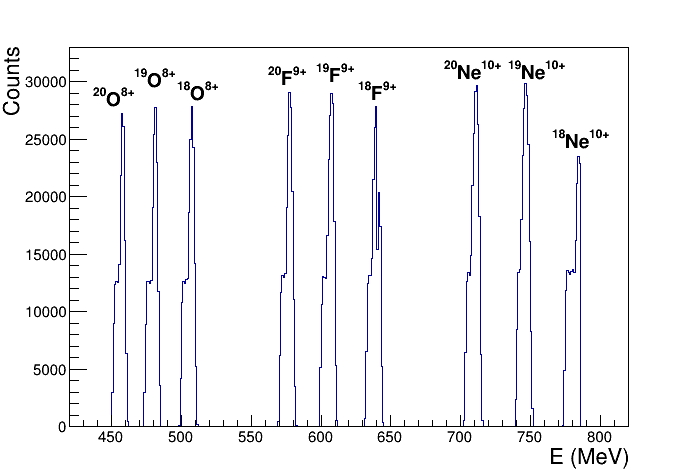
\includegraphics[width=\textwidth, keepaspectratio]{Grafici_Tesi2/PID/KinE2.png}
	%\vspace{7mm}
	%\subfigure[]
	%{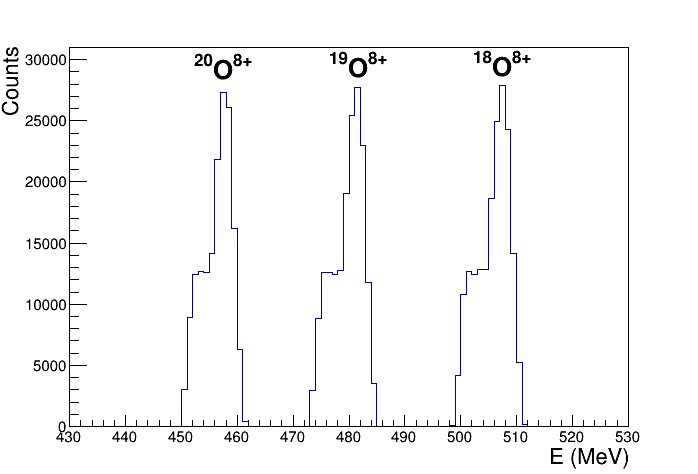
\includegraphics[scale=0.479]{Grafici_Tesi2/PID/KinE_zoom.png}}
	
	\caption{Lo spettro delle energie cinetiche~$E$ degli ioni simulati.} \label{fig:KinEa}
\end{figure}
Da tale figura si evince che le energie cinetiche accettate dal telescopio sono molto differenti per i diversi ioni, con una differenza fra lo ione più energetico e quello meno energetico di oltre 350~MeV.
%La Figura~\ref{fig:KinE}.b mostra un ingrandimento della precedente nella zona degli ioni di ossigeno: come si può notare, per ogni ione il range energetico che arriva sul telescopio è di circa 8~MeV, in buon accordo con la~\ref{eq:finestra_Brho}.
%Gli ioni hanno la stessa finestra di rigidità magnetica, per cui tutti vanno a finire sul telescopio simulato. 






Le corrispondenti matrici $\Delta E_{SiC} - E_{CsI}$ sono riportate in Figura~\ref{fig:deltaE_Ecsi_altaE}: come si può notare, i luoghi degli ioni simulati appaiono, anche in questo caso, ben separati sia in numero atomico sia in numero di massa.
Si può, inoltre, osservare che l'energia rilasciata nel rivelatore al~SiC è molto simile per le tre specie atomiche: 
%ciò dipende dalla notevole differenza in energia cinetica degli ioni che compensa la variazione legata al cambiamento di $Z$.
ciò dipende dal fatto che, a causa del filtro in $B \rho$, gli ioni con carica $q$ più piccola hanno energia cinetica minore, mentre quelli con $q$ più grande hanno energia cinetica maggiore; ricordando che nella formula di Bethe-Bloch la perdita di energia è proporzionale a $Z^2$ e inversamente proporzionale ad $E$, si può dedurre che la notevole differenza in energia cinetica degli ioni compensa la variazione legata al cambiamento di $Z$.
\begin{figure} [!p]
	\centering
	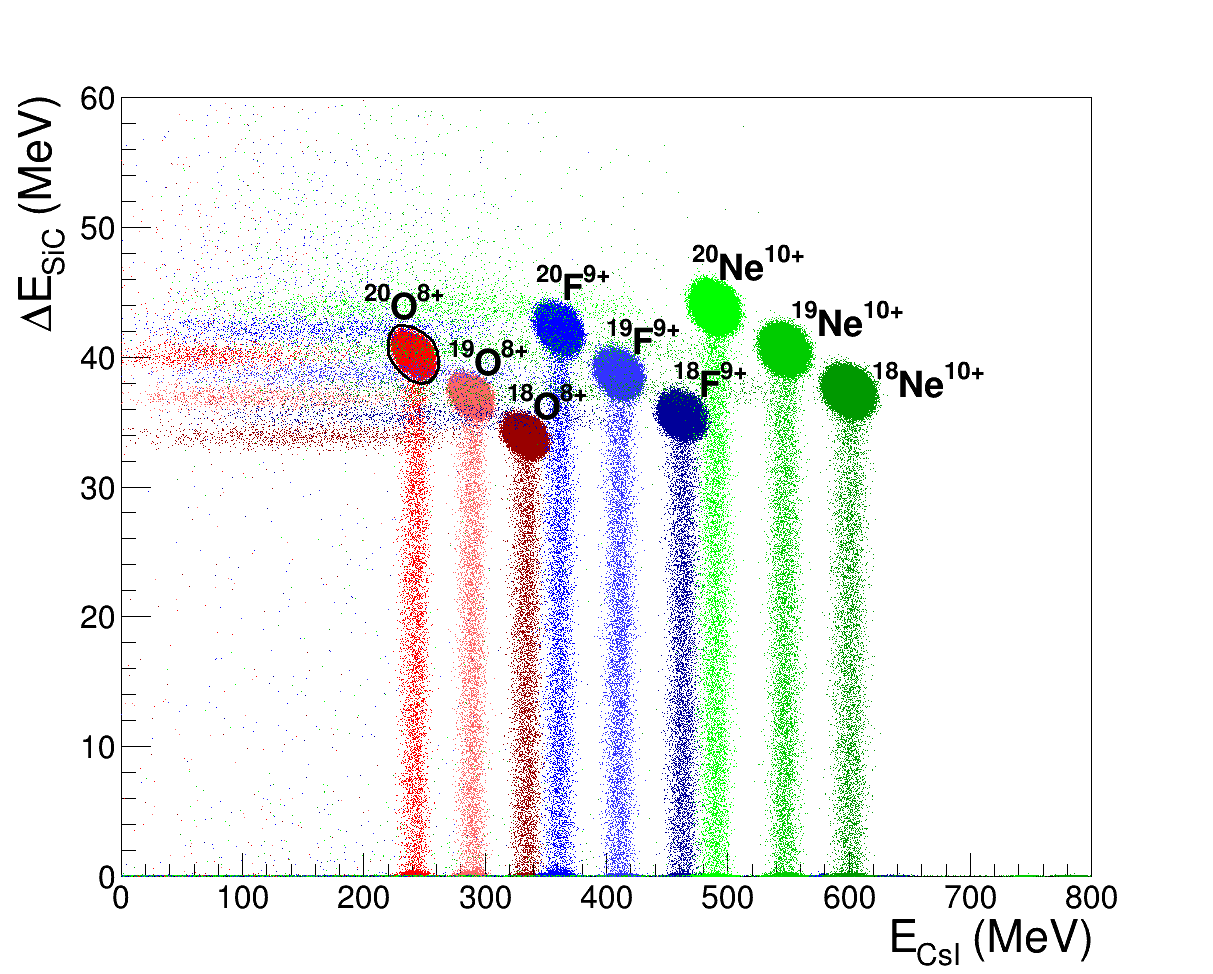
\includegraphics[width=\textwidth, keepaspectratio]{Grafici_Tesi2/PID/deltaE_Ecsi_quadrata_taglio_label.png}
	\caption{Le matrici $\Delta E_{SiC} - E_{CsI}$. Viene, inoltre, mostrato il taglio grafico per l'identificazione dell'\ce{^{20}O^{8+}} e per il calcolo delle percentuali di contaminazione.} \label{fig:deltaE_Ecsi_altaE}
\end{figure}
%Di conseguenza, assumendo di essere interessati ad una reazione di DCE in cui si vuole rivelare l'\ce{^{20}O}, la principale componente di contaminazione nell'identificazione proviene dagli ioni che non si fermano nel rivelatore al~CsI.
Di conseguenza, nel caso in esame la principale componente di contaminazione nell'identificazione degli eventi di interesse proviene dagli ioni che non si fermano nel cristallo di~CsI.

\begin{table} [t!]
	\begin{center}
		\renewcommand{\arraystretch}{1.2}
		\begin{tabular} {cccc}
			Ione               & & &   Contaminazione nella ROI (\%) \\
			\toprule[0.1em]
			%\hline
			\ce{^{18}O^{8+}}   & & &   0.0011 $\pm$ 0.0008 \\
			\hline
			\ce{^{19}O^{8+}}   & & &   0.0006 $\pm$ 0.0006 \\
			\hline
			\ce{^{18}F^{9+}}   & & &   0.013 $\pm$ 0.003 \\
			\hline
			\ce{^{19}F^{9+}}   & & &   0.082 $\pm$ 0.006 \\
			\hline
			\ce{^{20}F^{9+}}   & & &   0.042 $\pm$ 0.005 \\
			\hline
			\ce{^{18}Ne^{10+}} & & &   0.025 $\pm$ 0.004 \\
			\hline
			\ce{^{19}Ne^{10+}} & & &   0.078 $\pm$ 0.006 \\
			\hline
			\ce{^{20}Ne^{10+}} & & &   0.0009 $\pm$ 0.0006 \\
			\bottomrule[0.1em]
		\end{tabular}
	\end{center}
	\caption{La contaminazione dei diversi ioni nella ROI dell'\ce{^{20}O^{8+}} individuata dal taglio grafico in Figura~\ref{fig:deltaE_Ecsi_altaE}.} \label{tab:contaminazione_deltaE_Emeas_1.5per1.5a}
\end{table}
Le percentuali di contaminazione nella ROI individuata dal taglio grafico in Figura~\ref{fig:deltaE_Ecsi_altaE} sono riportate nella Tabella~\ref{tab:contaminazione_deltaE_Emeas_1.5per1.5a}: i contributi più rilevanti derivano dal \ce{^{19}F^{9+}} e dal \ce{^{19}Ne^{10+}}, come era lecito aspettarsi considerando che si tratta delle specie ioniche che hanno un valore di $\Delta E_{SiC}$ molto simile a quello dell'\ce{^{20}O^{8+}}.
%La percentuale di eventi di~\ce{^{20}O^{8+}} persi nell'identificazione può essere determinata dividendo il numero di eventi di~\ce{^{20}O^{8+}} al di fuori della ROI per il numero totale di eventi dello stesso: dal calcolo risulta che tale percentuale è del~$(9.14 \pm 0.08)$~\%.
L'efficienza di rivelazione del segnale è, in questo caso, pari al $(90.9 \pm 0.2)$~\%, in accordo con quelli precedentemente stimati.
%I valori tipici delle sezioni d'urto sperimentali dei processi coinvolti in questa simulazione, normalizzati alla sezione d'urto sperimentale peculiare del DCE, sono riportati nella Tabella~\ref{tab:sez_d'urtoa}, insieme alla probabilità di avere uno ione in un certo stato di carica dopo il passaggio attraverso un foglio di carbonio.
Nella Tabella~\ref{tab:sez_d'urtoa} sono riportati i valori tipici delle sezioni d'urto dei processi coinvolti, espressi relativamente alla sezione d'urto del DCE, e le probabilità dei diversi stati di carica.
%Moltiplicando il valore della sezione d'urto sperimentale tipica di un processo per la probabilità di ottenere uno stato di carica, si può determinare la probabilità di produrre, a seguito di una reazione nucleare, uno ione in un determinato stato di carica;
%%Moltiplicando i numeri della terza colonna con quelli della quarta, si può determinare la probabilità di ottenere, a seguito di una reazione nucleare, uno ione in un determinato stato di carica.
%questo è il fattore con cui bisogna riscalare le percentuali precedentemente mostrate per stimare le contaminazioni reali.
Analogamente a quanto visto in precedenza, sono stati ricavati i fattori di scala, i quali sono stati moltiplicati con i valori della Tabella~\ref{tab:sez_d'urtoa} per ottenere le contaminazioni reali.
Il risultato di questa operazione è riportato in Tabella~\ref{tab:contaminazioni_riscalatea}: come si può osservare, il contributo maggiore deriva dai processi di 1-neutron e 1-proton stripping e dal SCE.
Il rapporto S/B risulta essere di $0.0172 \pm 0.0008$, notevolmente inferiore ai valori precedentemente osservati.
\begin{table} [p!]
	\begin{center}
		\renewcommand{\arraystretch}{1.2}
		\begin{tabular} {cccccccl}
			Reazione & & Ione & & Sez. d'urto sperim.  & & \multicolumn{2}{c}{Fraz. di stato di carica}  \\
			& &      & &    norm. al DCE    & &&                          \\
			\toprule[0.1em]
			%\hline
			DCE        & & \ce{^{20}O}  & &        1        & & & $8^+ \sim 0.9987$ \\
			\hline
			SCE        & & \ce{^{20}F}  & &     $10^4$      & & & $9^+ \sim 0.99934$ \\
			& &              & &                 & & & $8^+ \sim 10^{-4}$ \\
			\hline
			1-proton   & & \ce{^{19}F}  & &  $2\cdot10^4 $  & & & $9^+ > 0.99934$ \\
			& &              & &                 & & & $8^+ < 10^{-4}$ \\
			\hline
			1-neutron  & & \ce{^{19}Ne} & &  $3\cdot10^4 $  & & & $10^+ > 0.99905$ \\
			& &              & &                 & & & $9^+ < 10^{-5}$ \\
			& &              & &                 & & & $8^+ < 10^{-7}$ \\
			\hline
			2-proton   & & \ce{^{18}O}  & &     $10^3$      & & & $8^+ > 0.99963$ \\
			\hline
			2-neutron  & & \ce{^{18}Ne} & &     $10^2 $     & & & $10^+ > 0.99905$ \\
			& &              & &                 & & & $9^+ < 10^{-5}$ \\
			& &              & &                 & & & $8^+ < 10^{-7}$ \\
			\hline
			1-deuteron & & \ce{^{18}F}  & &     $10^3 $     & & & $9^+ > 0.99934$ \\
			& &              & &                 & & & $8^+ < 10^{-4}$ \\
			\hline
			2-p 1-n    & & \ce{^{19}O}  & &        10       & & & $8^+ \sim 0.99963$ \\
			\hline
			inelastic  & & \ce{^{20}Ne} & &     $10^4 $     & & & $10^+ > 0.99905$ \\
			& &              & &                 & & & $9^+ < 10^{-5}$ \\
			& &              & &                 & & & $8^+ < 10^{-7}$ \\
			\bottomrule[0.1em]
		\end{tabular}
	\end{center}
	\caption{I valori tipici delle sezioni d'urto sperimentali di diversi processi di reazioni nucleari normalizzate alla sezione d'urto del DCE. Si riporta, inoltre, la probabilità di avere uno ione in un determinato stato di carica dopo aver attraversato un foglio di carbonio.} \label{tab:sez_d'urtoa}
\end{table}
\begin{table} [p!]
	\begin{center}
		\renewcommand{\arraystretch}{1.2}
		\begin{tabular} {cccc}
			Ione &  Stato di carica & & Numero di eventi nella ROI  \\
			&                  & &   norm. ad 1 evento di DCE  \\
			\toprule[0.1em]
			%\hline
			\ce{^{18}O}    &  $8^+$   & &  $0.017 \pm 0.010$      \\
			\hline
			\ce{^{19}O}    &  $8^+$   & &  $\sim 10^{-4}$  \\
			\hline
			\ce{^{20}O}    &  $8^+$   & &  $0.907 \pm 0.002$      \\
			\hline
			\ce{^{18}F}    &  $9^+$   & &  $0.17 \pm 0.03$        \\
			&  $8^+$   & &  $ \sim 10^{-6}$        \\
			\hline
			\ce{^{19}F}    &  $9^+$   & &  $20 \pm 1$             \\
			&  $8^+$   & &  $ < 0.0010 \pm 0.0001$    \\
			\hline
			\ce{^{20}F}    &  $9^+$   & &  $5.7 \pm 0.5$          \\
			\hline
			\ce{^{18}Ne}   &  $10^+$  & &  $0.031 \pm 0.004$      \\
			\hline
			\ce{^{19}Ne}   &  $10^+$  & &  $27 \pm 2$             \\
			\hline
			\ce{^{20}Ne}   &  $10^+$  & &  $0.14 \pm 0.08$        \\
			\bottomrule[0.1em]
		\end{tabular}
	\end{center}
	\caption{Per ogni ione si riporta il numero di eventi nella ROI normalizzato ad un evento di segnale.} \label{tab:contaminazioni_riscalatea}
\end{table}
La sensibilità di misura corrispondente è di circa 300~$\mu$b a 5$\sigma$, estremamente più grande di quella necessaria per osservare il DCE.
%Sebbene questo valore escluda la possibilità di riuscire a distinguere con il telescopio SiC-CsI le reazioni di DCE dal fondo, l'utilizzo di altre correlazioni potrebbe portare ad un miglioramento del rapporto S/B e, conseguentemente, ad un abbassamento della sensibilità di misura.
%Sebbene questo valore escluda la possibilità di riuscire a distinguere con il telescopio SiC-CsI le reazioni di DCE dal fondo, altre correlazioni potrebbero, invece, riuscire a separare il segnale dal rumore e, conseguentemente, 
Dunque, se si vuole effettuare uno studio delle reazioni di DCE ad elevate energie di eccitazione è necessario affiancare alla tecnica $\Delta E - E$ altre correlazioni, in grado di separare il segnale dai contaminanti; in tal modo, la sensibilità di misura complessiva dell'apparato potrebbe essere sufficiente per distinguere il DCE dal fondo.
Due importanti correlazioni sono descritte nel paragrafo successivo.


%\begin{table} [t!]
%	\begin{center}
%		\renewcommand{\arraystretch}{1.2}
%		\begin{tabular} {ccccccc}
%			Reazione & & Ione & & \multirow{2}{35 mm}{Sez. d'urto sperim. norm. al DCE}  & & Fraz. di stato di carica \\
%			         & &      & &        & &                          \\
%			\toprule
%			%\hline
%			DCE  & & \ce{^{20}O} & &  1  & & $8+ \rightarrow 0.9987$ \\
%			\hline
%			DCE  & & \ce{^{20}O} & &  1  & & $8+ \rightarrow 0.9987$ \\
%		\end{tabular}
%	\end{center}
%\end{table}
%\clearpage




%\clearpage
%\subsection*{Studio della correlazione $\Delta E_{SiC} - E_{CsI}$} 





%\subsection*{Studio delle correlazioni $x_{foc} - E_{CsI}$ e $\mbox{tof} - E_{CsI}$} 
\subsection*{\iflanguage{italian}{Studio delle correlazioni $x_{foc} - E_{CsI}$ e $\mbox{tof} - E_{CsI}$}{Study of $x_{foc} - E_{CsI}$ and $\mbox{tof} - E_{CsI}$ correlations}}
%A questo punto è interessante mostrare le correlazioni $x_{foc} - E$
%L'integrazione fra i software dedicati al trasporto ottico degli eiettili e la simulazione del telescopio permette di ricavare altre importanti correlazioni, utili per la PID.
%In Figura~ sono mostrate le matrici $x_{foc} - E_{meas}$ relative al caso in esame:

%Grazie all'utilizzo combinato delle correlazioni $\Delta E - E$ e di quelle originate dalla forza di Lorentz, l'attuale apparato sperimentale consente di identificare i prodotti di reazione sia in~$Z$ sia in rapporto $\sqrt{m}/q$ con elevata risoluzione.
%Nell'attuale apparato sperimentale i prodotti di reazione vengono identificati in numero atomico e in rapporto massa-carica grazie all'utilizzo congiunto della tecnica $\Delta E - E$ e della correlazione posizione-energia cinetica originata dalla forza di Lorentz.

%Come anticipato nel Paragrafo~\ref{sez:telescopi_sic_csi}, il progetto NUMEN intende svolgere l'identificazione in numero atomico, numero di massa e carica dei prodotti di reazione utilizzando congiuntamente la tecnica $\Delta E - E$, la correlazione posizione-energia cinetica originata dalla forza di Lorentz e la misura del tempo di volo.
%; allo scopo di studiare i processi di DCE è, infatti, fondamentale avere grandi capacità di PID per rigettare gli eventi di fondo.
%Nei paragrafi precedenti si è evidenziato come i telescopi SiC-CsI riescano a produrre nei plot $\Delta E - E$ un'efficace separazione degli ioni sia in $Z$ sia in $A$; tuttavia, utilizzando anche altre tipologie di correlazioni è possibile migliorare le capacità complessive di PID e la reiezione degli eventi di fondo. 
Il progetto NUMEN intende svolgere l'identificazione in numero atomico, numero di massa e carica dei prodotti di reazione utilizzando congiuntamente la tecnica $\Delta E - E$, la correlazione posizione-energia cinetica originata dalla forza di Lorentz e la misura del \emph{tempo di volo} (time of flight, tof).
%In questo paragrafo verranno esposti i risultati ottenuti dallo 
Per poter studiare, nell'ambito di questo lavoro, le ultime due tecniche di identificazione è stata di fondamentale importanza l'integrazione fra i software dedicati al trasporto ottico degli eiettili attraverso MAGNEX e la simulazione \geant{} del telescopio, in quanto ha permesso di ricavare tutte le osservabili necessarie per questo tipo di analisi. 
%L'integrazione fra i software dedicati al trasporto ottico degli eiettili e la simulazione del telescopio è stata fondamentale per ricavare le osservabili necessarie allo studio delle ultime due tecniche di identificazione.
%; in particolare, i primi contengono tutte le informazioni rilevanti  

Nel paragrafo~\ref{par:particelle_primarie} si è già discusso di come la misura in correlazione della coordinata orizzontale $x_{foc}$ al piano focale e dell'energia cinetica $E$ degli eiettili possa condurre all'identificazione di questi in $\sqrt{m}/q$ (si veda la~\ref{eq:legge_spettrometri_approx}).
L'utilità, ai fini della PID, della misura del tof viene, invece, discussa adesso: è ben noto che, in approssimazione non relativistica, l'energia cinetica $E$ di una particella di massa $m$ è legata alla sua velocità $v$ dalla relazione
\begin{equation} \label{eq:ekin}
	E \, = \, \frac{1}{2} \, m \, v^2
\end{equation}
La velocità $v$ è data da
\begin{equation} \label{eq:velocità}
v \, = \, \frac{d}{\mbox{tof}}
\end{equation}
laddove $d$ è la distanza percorsa dalla particella, chiamata \emph{base di volo}, e tof è l'intervallo di tempo impiegato a coprire tale distanza.
Sostituendo la~\ref{eq:velocità} nella~\ref{eq:ekin} si trova
\begin{equation} \label{eq:tof_ekin}
E \, = \, \frac{1}{2} \, m \, \frac{d^2}{\mbox{tof}^2}
\end{equation}
Pertanto, nota la base di volo della particella, misurando in correlazione l'energia cinetica e il tempo di volo è possibile ricavarne la massa; la misura del tof consente, dunque, di identificare in massa i prodotti di reazione.

%Sebbene sia la~\ref{eq:legge_spettrometri_approx} sia la~\ref{eq:tof_ekin} richiedano la misura dell'energia cinetica~$E$, se la perdita di energia $\Delta E$ della particella attraversando il primo stadio di un telescopio è piccola, allora 
Si fa notare che sia la~\ref{eq:legge_spettrometri_approx} sia la~\ref{eq:tof_ekin} richiedono la misura dell'energia cinetica~$E$; d'altro canto,  si è già visto che nel sistema di rivelazione considerato non abbiamo accesso a tale quantità a causa della presenza del substrato passivato del rivelatore al~SiC.
Inoltre, nel paragrafo precedente si è mostrato che, se nelle correlazioni $\Delta E - E$ si utilizza l'energia $E_{CsI}$ misurata dal cristallo di~CsI invece di $E_{meas}$, le capacità di PID restano elevate.
Per questo motivo, nel prosieguo verranno trattate soltanto le correlazioni che coinvolgono $E_{CsI}$ piuttosto che l'energia cinetica~$E$.
Ovviamente, se la perdita di energia $\Delta E$ è piccola rispetto ad~$E$, $E_{CsI}$ ed $E$ sono molto simili.

\begin{figure} [!p]
	\centering
	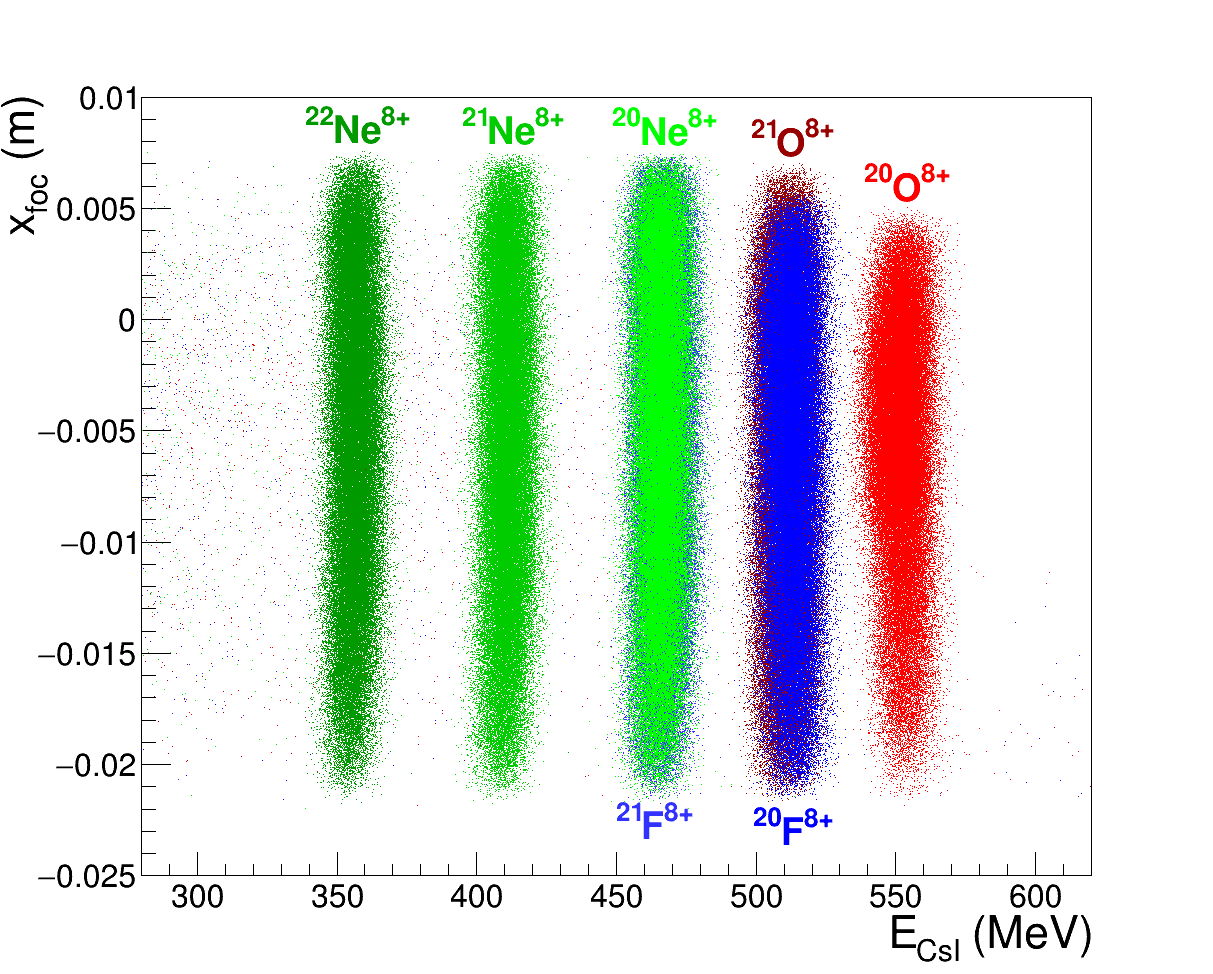
\includegraphics[width=\textwidth, keepaspectratio]{Grafici_Tesi2/PIDnew/xf_csi_label_quadrata_menoeventi2.png}
	\caption{Le tipiche matrici $x_{foc} - E_{CsI}$.} \label{fig:xf_Ecsi}
\end{figure}

Le matrici $x_{foc} - E_{CsI}$ corrispondenti alla simulazione della Sezione~\ref{sez:studio_PID} sono riportate in Figura~\ref{fig:xf_Ecsi}: come si può notare, gli ioni si dispongono su luoghi diversi a secondo del loro rapporto~$\sqrt{m}/q$. 
I luoghi sono ben separati, ad eccezione, ovviamente, di quelli con lo stesso rapporto massa su carica.
%Ciò poteva essere già dedotto guardando la Figura~\ref{fig:deltaE_Ecsi}, in cui si può notare che le matrici delle coppie in questione hanno intervalli di energia $E_{CsI}$ in parte sovrapposti.
%Con lo stesso tipo di ragionamento, osservando la Figura~\ref{fig:deltaE_Ecsi_stati_carica}, si può desumere che se, oltre agli ioni considerati, si fossero simulati anche il \ce{^{18}F^{8+}} e il \ce{^{19}F^{8+}}, allora le matrici di questi due ioni si sarebbero in parte sovrapposta al luogo dell'\ce{^{20}O^{8+}}.
È interessante sottolineare che, nonostante il telescopio abbia una lunghezza di 1.5~cm, esso vede un intervallo di $x_{foc}$ di circa 2.8~cm; ciò deriva dal fatto che gli ioni possono incidere sul telescopio con un certo angolo orizzontale non nullo, aumentando il numero di traiettorie accettate dal dispositivo.
Inoltre, in Figura~\ref{fig:xf_Ecsi} è evidente la presenza di eventi degradati, che anche in questo caso possono andare a posizionarsi sui luoghi di altri ioni.
%; dunque, anche in questa rappresentazione la specie ionica di interesse sarebbe affetta da contaminazioni.

%Nella procedura di identificazione degli ioni effettuata con l'attuale apparato sperimentale, 
L'identificazione dei prodotti di reazione rivelati con l'attuale apparato sperimentale viene svolta effettuando dapprima un taglio grafico nei plot $\Delta E - E_{resid}$ per selezionare in $Z$ la specie di interesse; dopo di che, gli eventi così selezionati vengono riportati in un grafico $x_{foc} - E_{resid}$ per separare i diversi isotopi e stati di carica. 
\begin{figure} [!p]
	\centering
	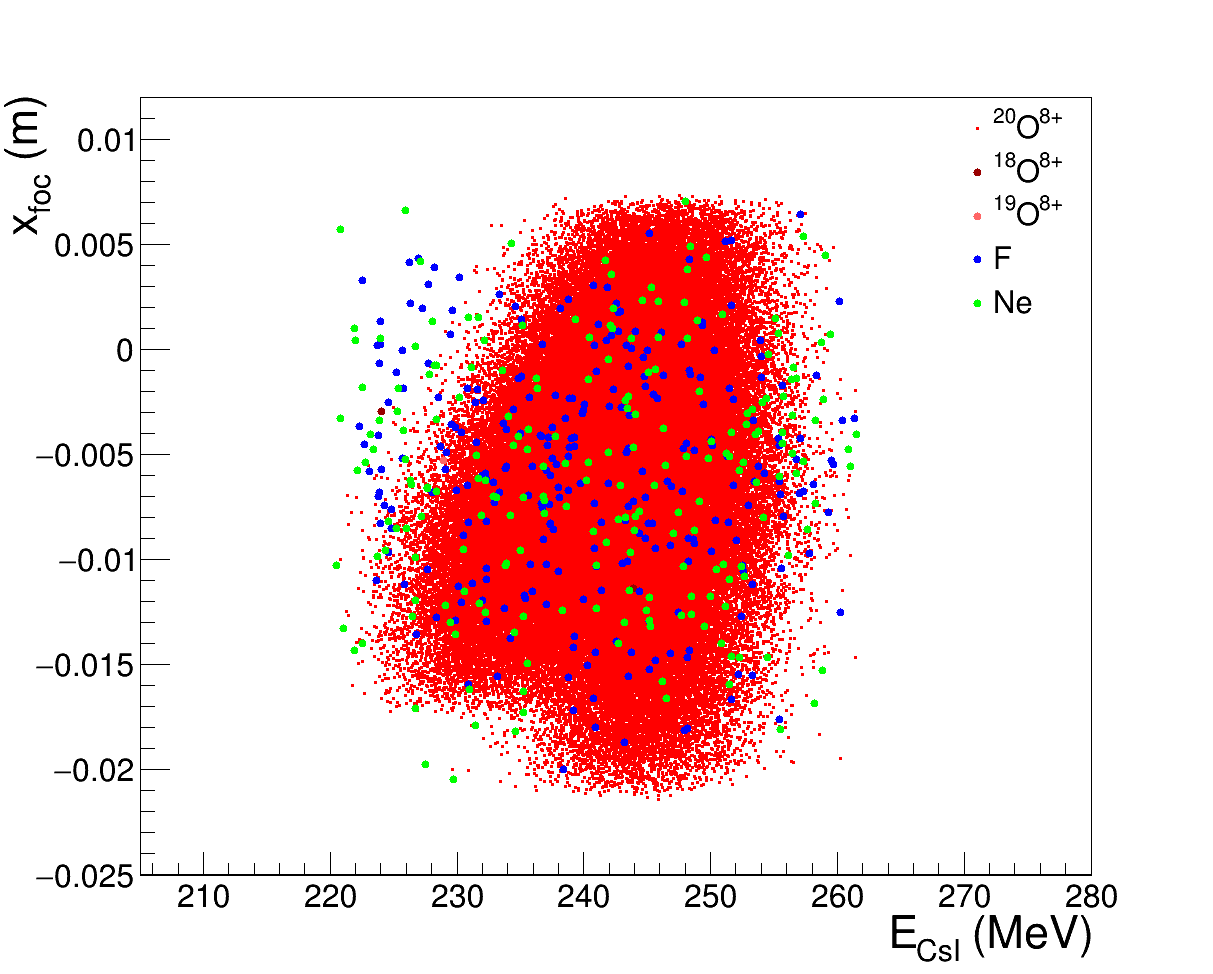
\includegraphics[width=\textwidth, keepaspectratio]{Grafici_Tesi2/PID/xf_csi_taglio2.png}
	\caption{La matrice $x_{foc} - E_{CsI}$ per gli eventi selezionati dal taglio grafico in Figura~\ref{fig:deltaE_Ecsi_altaE}.} \label{fig:xf_Ecsi_O20a}
\end{figure}
\begin{figure} [!p]
	\centering
	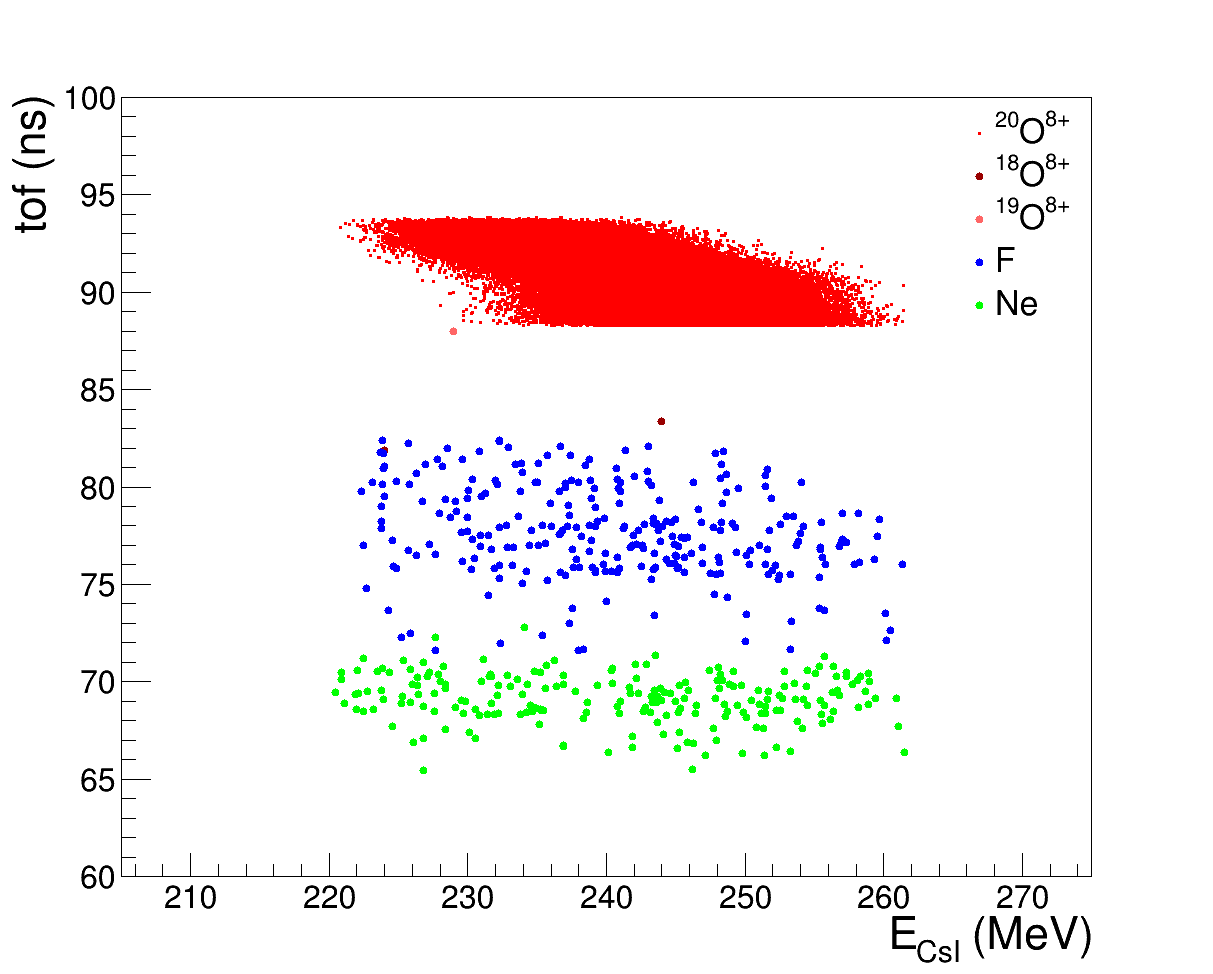
\includegraphics[width=\textwidth, keepaspectratio]{Grafici_Tesi2/PIDnew/tof_csi_taglio2.png}
	\caption{La matrice $\mbox{tof} - E_{CsI}$ per gli eventi selezionati dal taglio grafico in Figura~\ref{fig:deltaE_Ecsi_altaE}.} \label{fig:tof_Ecsi_O20a}
\end{figure} 
%La simulazione svolta per questo lavoro ha dimostrato che il telescopio SiC-CsI è in grado, da solo, di identificare lo ione di interesse sia in $Z$ sia in $A$, rendendo, dunque, in linea di principio non necessaria la rappresentazione degli eventi nel plot $x_{foc} - E_{CsI}$.
%Tuttavia, nel caso esposto in Figura~\ref{fig:deltaE_Ecsi} si vede come il telescopio SiC-CsI possa essere in grado, da solo, di identificare lo ione di interesse sia in $Z$ sia in $A$; di conseguenza, la rappresentazione de
Tuttavia, nel caso esposto in Figura~\ref{fig:deltaE_Ecsi_altaE} si vede come il taglio grafico sia stato, da solo, sufficiente ad identificare lo ione di interesse sia in $Z$ sia in $A$; dunque, riportando gli eventi selezionati in un grafico $x_{foc} - E_{CsI}$ non si dovrebbero osservare altri luoghi se non quello dell'\ce{^{20}O^{8+}}.
Questa affermazione viene confermata dalla Figura~\ref{fig:xf_Ecsi_O20a}, dove è possibile vedere soltanto la matrice dello ione di interesse.
Sovrapposti a tale matrice, si possono notare gli eventi degradati dell\ce{^{20}O^{8+}} che contaminano il segnale: purtroppo la rappresentazione $x_{foc} - E_{CsI}$ non risulta utile, in questo caso, a separare lo ione di interesse dai contaminanti.
%, in quanto questi hanno un'energia $E_{CsI}$ uguale a quella del segnale.

Per cercare di separare il segnale dal fondo si può, allora, pensare di utilizzare la correlazione $\mbox{tof} - E_{CsI}$: in Figura~\ref{fig:tof_Ecsi_O20a}, dove sono riportati gli eventi selezionati dal taglio grafico in Figura~\ref{fig:deltaE_Ecsi_altaE}, è possibile notare come questa rappresentazione permetta di distinguere chiaramente il segnale dagli ioni F e Ne.
%Ricordando che, a causa delle diverse sezioni d'urto dei processi, queste due specie 
%Ricordando la Tabella~\ref{tab:contaminazioni_deltaE_Ecsi_riscalate}, queste due specie danno il maggiore contributo di contaminazione nella ROI, avendo delle sezioni d'urto estremamente più grandi 
Si ricorda che queste due specie, a causa della loro elevata sezione d'urto, danno il maggiore contributo di contaminazione nella ROI (si veda la Tabella~\ref{tab:contaminazioni_deltaE_Ecsi_riscalate}); di conseguenza, riuscire a isolarle dal segnale consentirebbe di aumentare il rapporto S/B e di diminuire la sensibilità di misura complessiva dell'apparato.
%È bene sottolineare che al momento sulla variabile tof non vengono considerate né le fluttuazioni statistiche né gli eventi spuri originati da coincidenze casuali, che contribuirebbero ad allargare le matrici e ad introdurre una ulteriore componente di fondo.
È bene sottolineare che al momento la variabile tof viene determinata con calcoli analitici dai software per il trasporto ottico e non incorpora le fluttuazioni statistiche tipiche del processo di misura, le quali contribuirebbero ad allargare le matrici.
Tuttavia, la Figura~\ref{fig:tof_Ecsi_O20a} può fornire un'indicazione della precisione minima necessaria per riuscire a separare lo ione di interesse dal fondo: osservando la figura, si può dedurre che essa deve essere inferiore a 10~ns, altrimenti gli eventi originati dal F potrebbero sovrapporsi a quelli dell'\ce{^{20}O^{8+}}.

%Dal momento che queste due specie, a causa della loro elevata sezione d'urto di produzione, danno il maggiore contributo di contaminazione nella ROI (si veda la Tabella~\ref{tab:contaminazioni_deltaE_Ecsi_riscalate}), riuscire a 
%È bene sottolineare che nel grafico mostrato, 
%Alla luce di questo risultato, si deduce che la misura del tempo di volo è fondamentale per migliorare le capacità di PID complessive dell'apparato.
%Alla luce di questo risultato, si deduce che la misura del tempo di volo è fondamentale per migliorare le capacità di PID complessive dell'apparato e per aumentare la sensibilità di misura della reazione di interesse. 
Alla luce delle considerazioni effettuate, risulta che la misura del tempo di volo è fondamentale per poter analizzare le reazioni di DCE ad elevata energia di eccitazione.



 


%\clearpage
\subsection{\iflanguage{italian}{Studio della granularità}{Study of granularity}}

%Uno degli obiettivi fondamentali di questo lavoro di tesi consiste nell'ottimizzazione delle dimensioni trasversali dei telescopi, al fine di minimizzare la percentuale di eventi in cui la carica è stata raccolta parzialmente. 
Uno degli obiettivi fondamentali di questo lavoro di tesi consiste nell'ottimizzazione delle dimensioni trasversali dei telescopi, valutando per diverse soluzioni le percentuali di contaminazione e il rapporto S/B.
%Dal momento che la lunghezza della cornice completamente inattiva e della regione di transizione dovrebbero essere circa costanti pur variando la superficie del rivelatore al~SiC, ci si aspetta che all'aumentare delle dimensioni trasversali del telescopio la frazione degli eventi con raccolta di carica incompleta diminuisca.
%È importante sottolineare che, in accordo con la~\ref{eq:finestra_Brho}, variando la dimensione orizzontale del telescopio, cambia la finestra in $B \rho$ accettata e, di conseguenza, per ogni ione cambia l'intervallo di energia cinetica.
%Poiché lo spettro in energia cinetica dipende dal tipo di ione, 
%È importante sottolineare che, nonostante la rigidità magnetica di riferimento resti la stessa, in accordo con la~\ref{eq:finestra_Brho}, variando la larghezza del telescopio cambia la finestra in $B \rho$ accettata. 
%Poiché il corrispondente intervallo di energia cinetica dipende dallo ione, tale cambiamento si manifesta in misura diversa su specie ioniche differenti.
È importante sottolineare che, nonostante la rigidità magnetica di riferimento resti la stessa, in accordo con la~\ref{eq:finestra_Brho}, variando la larghezza del telescopio, cambia la finestra in $B \rho$ accettata e, di conseguenza, cambia per ogni ione l'intervallo di energia cinetica accettato.
Poiché lo spettro in energia cinetica non è uniforme ma ha una forma complessa che dipende dal tipo di ione (si veda la Figura~\ref{fig:KinEa}), tale cambiamento si manifesta in misura diversa su specie ioniche differenti.
Pertanto, non è banale prevedere il comportamento del rapporto S/B al variare delle diverse configurazioni.

Tenendo presenti gli attuali limiti imposti dal processo di produzione dei rivelatori al~SiC, sono stati esaminati tre casi: $1 \times 1$, $1.5 \times 1.5$ e $2 \times 2$~cm\ap{2}. 
Dal momento che per l'analisi delle reazioni di DCE la regione di interesse è quella a bassa energia di eccitazione, in ciascuna delle tre possibilità le particelle primarie sono state generate mantenendo i parametri elencati nel Paragrafo~\ref{sez:studio_PID}.
Per quanto riguarda i telescopi da 1.5~cm $\times$ 1.5~cm, i plot e le tabelle di riferimento sono quelli mostrati nella sezione precedente, mentre per gli altri due vengono adesso esposti.


\subsection*{Dimensioni trasversali: 1~cm $\times$ 1~cm}
%\paragraph*{Dimensioni trasversali: 1.5~cm $\times$ 1.5~cm.}
%Come si può notare dalla Figura~\ref{fig:deltaE_ERes_1.5}, le matrici $\Delta E_{SiC} - E_{CsI}$ nel caso in esame 
%Poiché nel caso in esame le matrici $\Delta E_{SiC} - E_{CsI}$ continuano ad essere ben separate e non mostrano variazioni percettibili rispetto a quelle in Figura~\ref{fig:deltaE_ERes_adron}, si è scelto di non riportarle.
%Ciò viene corroborato anche dalla Figura~\ref{fig:xf_ecsi_1per1}, in cui si osserva che l'intervallo di valori di $x_{foc}$ visto dal telescopio è di circa 2.3~cm, inferiore di 


%%%Riducendo la dimensione orizzontale del telescopio dovrebbe diminuire il range di energie cinetiche accettato: in effetti, confrontando la Figura~\ref{fig:ekin_1per1} con la~\ref{fig:KinE} si può notare che i picchi dei diversi ioni sono più stretti. Ciò viene corroborato anche dal confronto tra la Figura~\ref{fig:xf_ecsi_1per1} e la~\ref{fig:xf_Ecsi}; infatti, nella prima si osserva che l'intervallo di valori di $x_{foc}$ visto dal telescopio è di circa 2.3~cm, mentre nella seconda tale intervallo è di 2.8~cm. Poiché negli spettrometri magnetici vi è una relazione di proporzionalità tra la posizione degli eiettili al piano focale e la loro energia cinetica, se ne deduce che nel primo caso l'intervallo di energia cinetica visto dal telescopio è più piccolo.


\begin{figure} [!p]
	\centering
	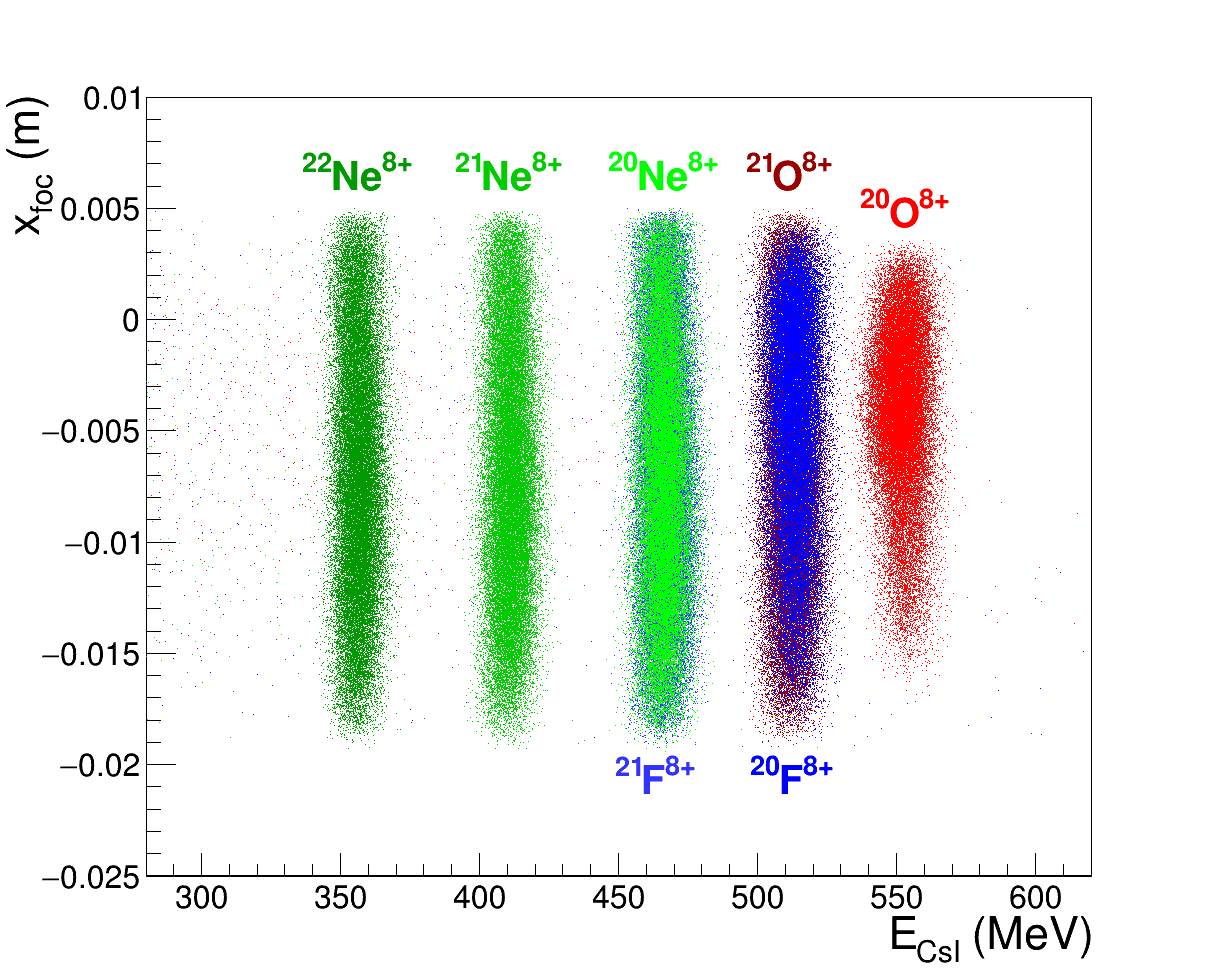
\includegraphics[width=\textwidth, keepaspectratio]{Grafici_Tesi2/1per1new/xf_ecsi_quadrata_menoeventi.png}
	\caption{Le matrici $x_{foc} - E_{CsI}$ nel caso in cui le dimensioni trasversali del telescopio siano di 1~cm~$\times$~1~cm.} \label{fig:xf_ecsi_1per1}
\end{figure} 

Riducendo la dimensione orizzontale del telescopio dovrebbe diminuire il range di energie cinetiche accettato: in effetti, confrontando la Figura~\ref{fig:xf_ecsi_1per1} e la Figura~\ref{fig:xf_Ecsi} si può notare che mentre nella prima l'intervallo di~$x_{foc}$ visto dal telescopio è di circa 2.3~cm, nella seconda tale intervallo è di 2.8~cm. Poiché negli spettrometri magnetici vi è una relazione di proporzionalità tra la posizione degli eiettili al piano focale e la loro energia cinetica, se ne deduce che nel primo caso l'intervallo di energia cinetica visto dal telescopio è più piccolo.
 
%\begin{figure} [!p]
%	\centering
%	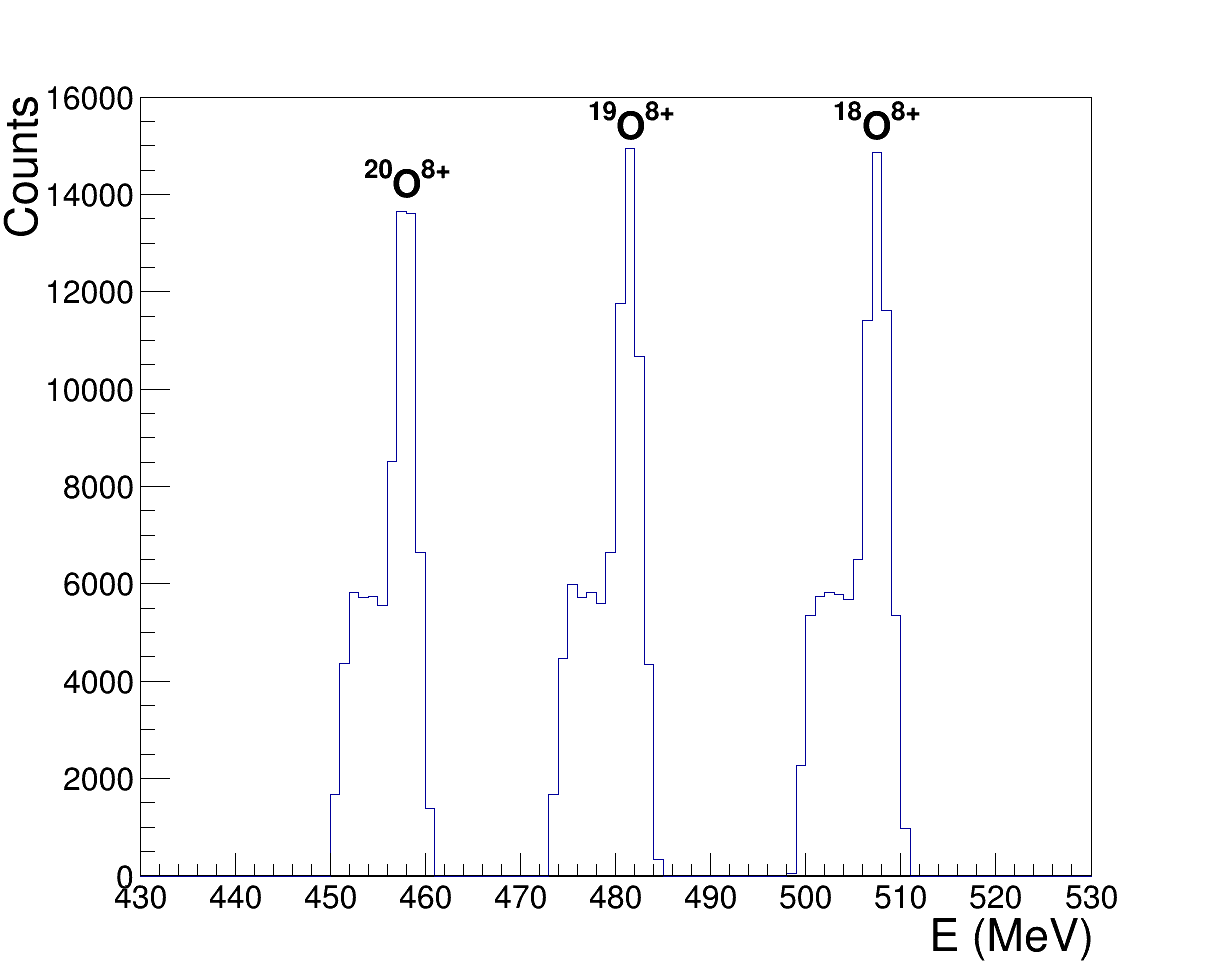
\includegraphics[width=\textwidth, keepaspectratio]{Grafici_Tesi2/1per1/e_kin_ossigeno_quadrata.png}
%	\caption{Lo spettro in energia cinetica degli ioni ossigeno nel caso in cui le dimensioni trasversali del telescopio siano di 1~cm~$\times$~1~cm.} \label{fig:ekin_1per1}
%\end{figure} 





\begin{table} [t!]
	\begin{center}
		\renewcommand{\arraystretch}{1.2}
		\begin{tabular} {cccc}
			Ione &  Stato di carica & & Numero di eventi nella ROI  \\
			&                  & &   norm. ad 1 evento di DCE  \\
			\toprule[0.1em]
			%\hline
			\ce{^{20}O}    &  $8^+$   & &  $0.884 \pm 0.003$      \\
			\hline
			\ce{^{21}O}    &  $8^+$   & &  $\sim 8 \cdot 10^{-6}$      \\
			\hline
			\ce{^{20}F}    &  $8^+$   & &  $< 2 \cdot 10^{-4}$ al 90\% CL       \\
			\hline
			\ce{^{21}F}    &  $8^+$   & &  $< 10^{-7} $ al 90\% CL     \\
			\hline
			\ce{^{20}Ne}    &  $8^+$   & &  $< 10^{-8}$ al 90\% CL        \\
			\hline
			\ce{^{21}Ne}   &  $8^+$  & &  $< 10^{-7} $  al 90\% CL    \\
			\hline
			\ce{^{22}Ne}   &  $8^+$  & &  $< 10^{-9}$    al 90\% CL    \\
			\bottomrule[0.1em]
		\end{tabular}
	\end{center}
	\caption{Dimensioni del telescopio 1~cm $\times$ 1~cm: utilizzando la correlazione $\Delta E_{SiC} - E_{CsI}$, per ogni ione si riporta il numero di eventi nella ROI normalizzato ad un evento di segnale.} \label{tab:contaminazioni_deltaE_Ecsi_riscalate_1per1}
\end{table}

%In Figura~\ref{fig:deltaE_Ecsi_1per1} vengono illustrate le matrici $\Delta E_{SiC} - E_{CsI}$ ottenute con questa configurazione: rispetto alla Figura~\ref{fig:deltaE_Ecsi} non si osservano differenze sostanziali.
%\begin{figure} [!p]
%	\centering
%	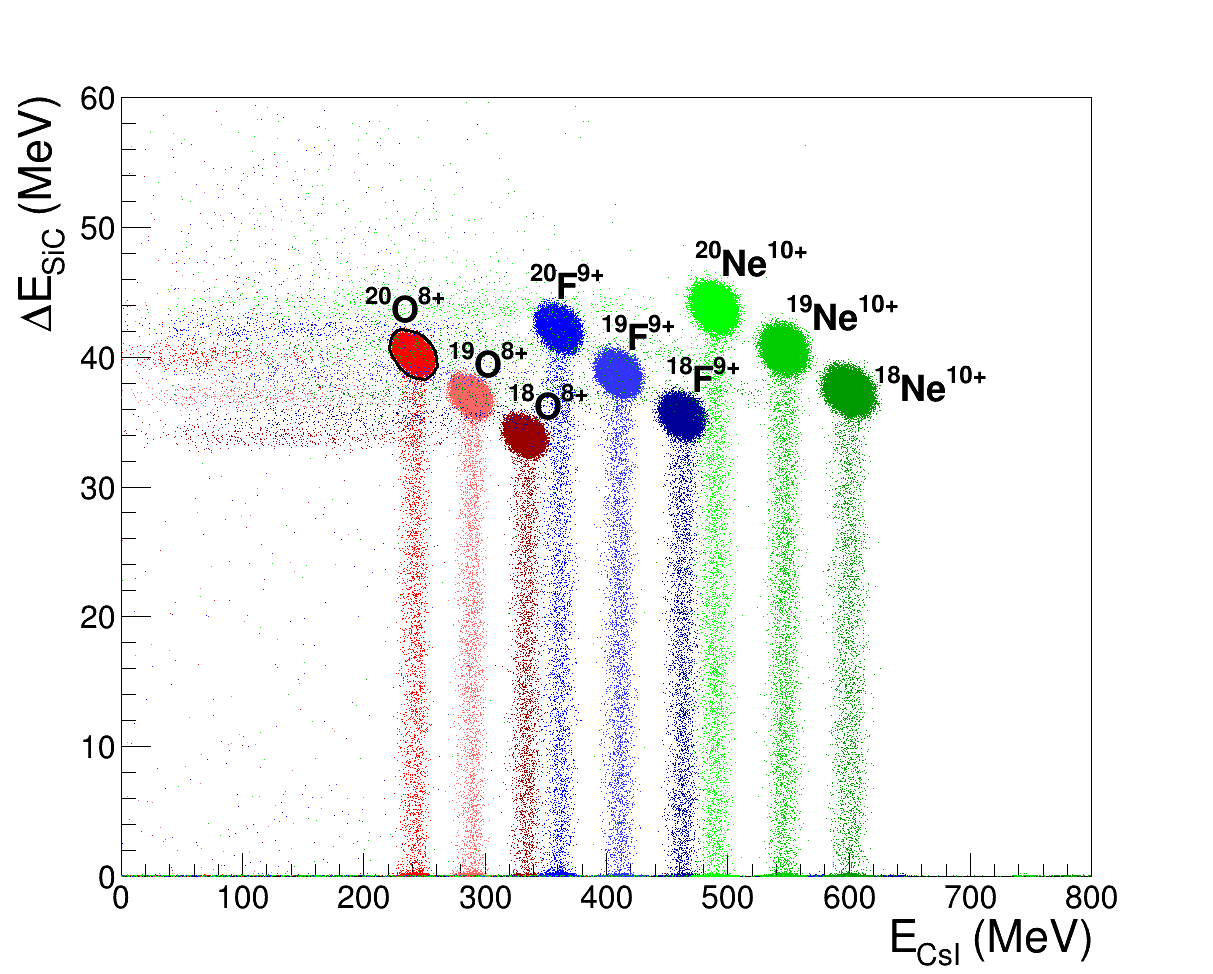
\includegraphics[width=\textwidth, keepaspectratio]{Grafici_Tesi2/1per1/deltaE_Ecsi_taglio.png}
%	\caption{Le matrici $\Delta E_{SiC} - E_{CsI}$ nel caso in cui le dimensioni trasversali del telescopio siano di 1~cm~$\times$~1~cm. Viene, inoltre, mostrato il taglio grafico per l'identificazione dell'\ce{^{20}O^{8+}} e per il calcolo delle percentuali di contaminazione} \label{fig:deltaE_Ecsi_1per1}
%\end{figure}
Dal momento che le matrici $\Delta E_{SiC} - E_{CsI}$ continuano ad essere ben separate e non presentano variazioni percettibili rispetto a quelle in Figura~\ref{fig:deltaE_Ecsi}, si è scelto di non mostrarle.
Nella Tabella~\ref{tab:contaminazioni_deltaE_Ecsi_riscalate_1per1} si riporta il numero di eventi nella ROI, riscalato per la sezione d'urto e per la probabilità di ottenere un certo stato di carica e normalizzato ad un evento di DCE: confrontando questa con la Tabella~\ref{tab:contaminazioni_deltaE_Ecsi_riscalate} si può notare che le contaminazioni sono leggermente più alte, mentre l'efficienza di rivelazione del segnale è più bassa, risultando essere dell'$(88.4 \pm 0.3)$~\%.
Calcolando il rapporto S/B si trova un valore di $4875 \pm 19$, minore di quello trovato nel caso precedente.
La sensibilità di misura risulta essere di 1~nb a 5$\sigma$, dunque anche in questo caso sufficiente per rivelare la reazione di interesse.





\subsection*{Dimensioni trasversali: 2~cm $\times$ 2~cm}
%\paragraph*{Dimensioni trasversali: 2~cm $\times$ 2~cm.}

In questo caso, l'intervallo di energia cinetica accettato dal telescopio è maggiore, come viene confermato dalla Figura~\ref{fig:xf_ecsi_2per2}, in cui si può notare che l'intervallo di $x_{foc}$ visto dal telescopio è di circa 3.4~cm.
\begin{figure} [!p]
	\centering
	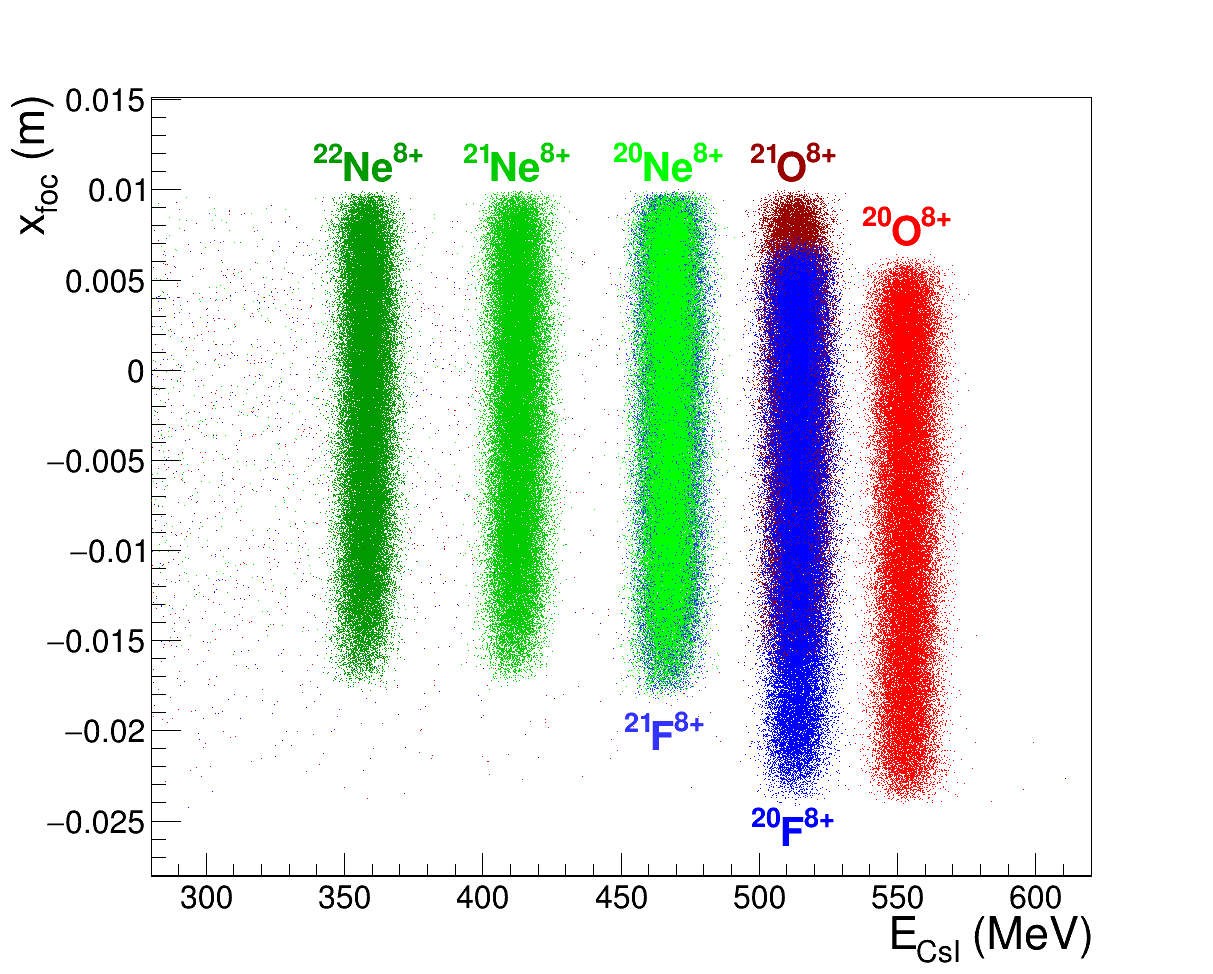
\includegraphics[width=\textwidth, keepaspectratio]{Grafici_Tesi2/2per2new/xf_ecsi_quadrata_menoeventi.png}
	\caption{Le matrici $x_{foc} - E_{CsI}$ nel caso in cui le dimensioni trasversali del telescopio siano di 2~cm~$\times$~2~cm.} \label{fig:xf_ecsi_2per2}
\end{figure} 
Per i motivi precedentemente esposti, anche in questo caso si è preferito non riportare le matrici $\Delta E_{SiC} - E_{CsI}$.
Il numero di eventi nella ROI, riscalato per la sezione e per la probabilità di ottenere un determinato stato di carica e normalizzato ad un evento di DCE, viene mostrato, per ogni ione, nella Tabella~\ref{tab:contaminazioni_deltaE_Ecsi_riscalate_2per2}: come si può notare, i valori sono più alti di quelli visti nelle altre due condizioni.
\begin{table} [t!]
	\begin{center}
		\renewcommand{\arraystretch}{1.2}
		\begin{tabular} {cccc}
			Ione &  Stato di carica & & Numero di eventi nella ROI  \\
			&                  & &   norm. ad 1 evento di DCE  \\
			\toprule[0.1em]
			%\hline
			\ce{^{20}O}    &  $8^+$   & &  $0.917 \pm 0.002$      \\
			\hline
			\ce{^{21}O}    &  $8^+$   & &  $\sim 8 \cdot 10^{-6}$      \\
			\hline
			\ce{^{20}F}    &  $8^+$   & &  $< 5 \cdot 10^{-5}$ al 90\% CL       \\
			\hline
			\ce{^{21}F}    &  $8^+$   & &  $< 10^{-7} $ al 90\% CL     \\
			\hline
			\ce{^{20}Ne}    &  $8^+$   & &  $< 10^{-8}$ al 90\% CL        \\
			\hline
			\ce{^{21}Ne}   &  $8^+$  & &  $< 10^{-7} $  al 90\% CL    \\
			\hline
			\ce{^{22}Ne}   &  $8^+$  & &  $< 10^{-9}$    al 90\% CL    \\
			\bottomrule[0.1em]
		\end{tabular}
	\end{center}
	\caption{Dimensioni del telescopio 2~cm $\times$ 2~cm: utilizzando la correlazione $\Delta E_{SiC} - E_{CsI}$, per ogni ione si riporta il numero di eventi nella ROI normalizzato ad un evento di segnale.} \label{tab:contaminazioni_deltaE_Ecsi_riscalate_2per2}
\end{table}
%L'efficienza di rivelazione del segnale è maggiore rispetto ai casi precedenti, raggiungendo il $(91.9 \pm 0.002)$~\%.
%Il rapporto S/B risulta essere pari a $0.0020 \pm 0.001$, diminuend 
Rispetto ai due casi precedenti, l'efficienza di rivelazione del segnale è maggiore, raggiungendo il $(91.7 \pm 0.2)$~\%.
Anche il rapporto S/B risulta maggiore, con un valore di $16530 \pm 32$.
Ciò significa che, aumentando le dimensioni trasversali del telescopio, aumenta il numero di segnali presenti nella ROI, mentre il fondo, in proporzione, diminuisce.
Calcolando la sensibilità di misura, si trova un valore di 300~pb a 5$\sigma$, più basso rispetto ai due precedenti. 






%\begin{figure} [!p]
%	\centering
%	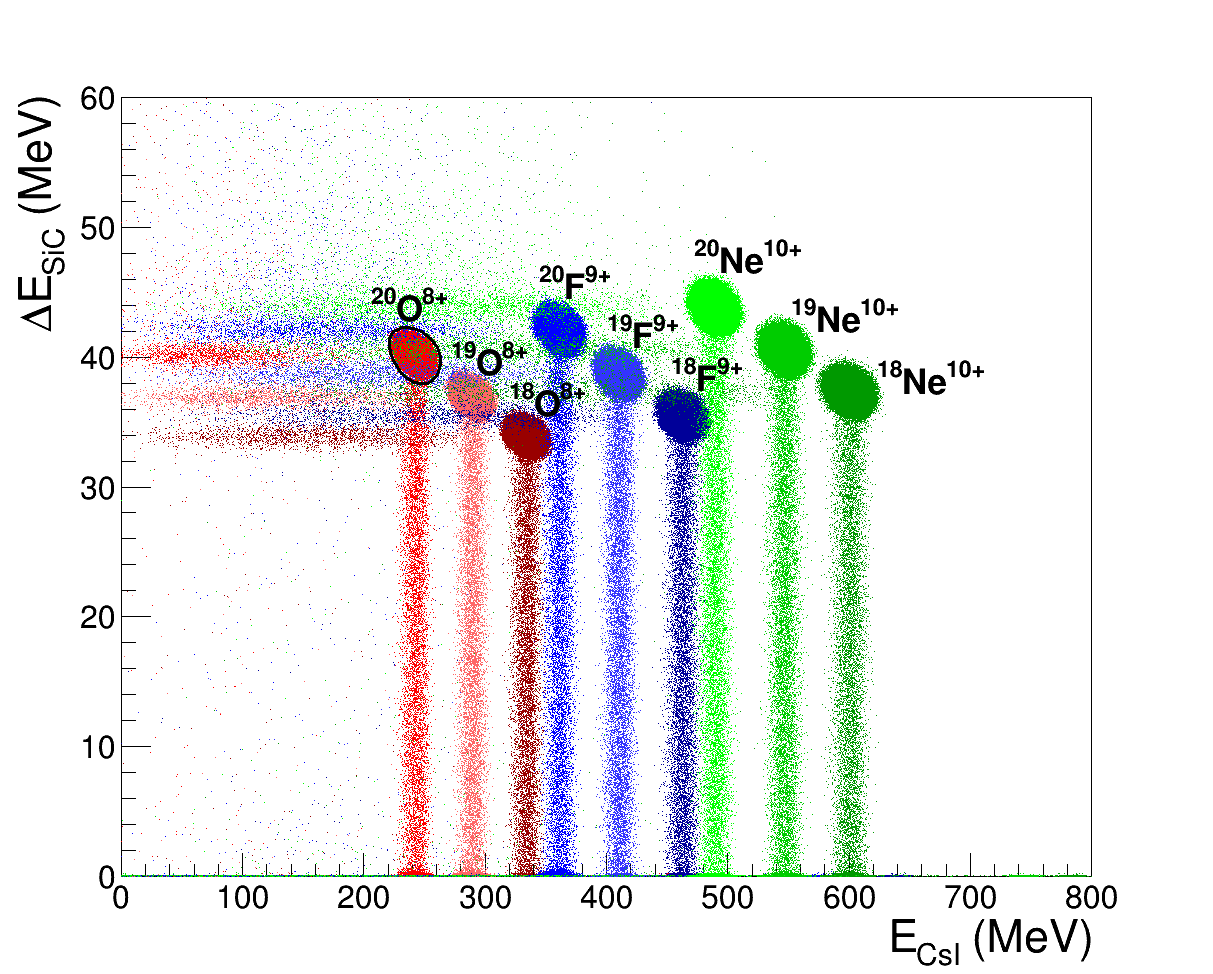
\includegraphics[width=\textwidth, keepaspectratio]{Grafici_Tesi2/2per2new/deltaE_Ecsi_taglio.png}
%	\caption{Le matrici $\Delta E_{SiC} - E_{CsI}$ nel caso in cui le dimensioni trasversali del telescopio siano di 1~cm~$\times$~1~cm. Viene, inoltre, mostrato il taglio grafico per l'identificazione dell'\ce{^{20}O^{8+}} e per il calcolo delle percentuali di contaminazione} \label{fig:deltaE_Ecsi_2per2}
%\end{figure} 






\subsection*{Conclusioni}


%In accordo con quanto trovato, si può affermare che, al fine di minimizzare gli eventi con raccolta di carica incompleta, è opportuno avere la maggiore superficie di rivelazione possibile.
%Ciò si può evincere dalla Figura~\ref{fig:misident_vs_surface}, dove è mostrato, per un caso rappresentativo, l'andamento della probabilità di errore nell'identificazione dei nuclei al variare della superficie e dell'energia.
%Ciò si spiega considerando che, a parità di lunghezza della cornice, aumentando l'area del rivelatore cresce la frazione di superficie sensibile rispetto a quella totale.
%Tale andamento può essere spiegato considerando che, a parità di lunghezza della cornice non attiva, aumentando l'area del rivelatore cresce la frazione di superficie sensibile rispetto a quella totale.
Lo studio effettuato ha dimostrato che, aumentando le dimensioni trasversali del telescopio, cresce il rapporto S/B e, di conseguenza, diminuisce il valore della sezione d'urto minima rivelabile; l'andamento di quest'ultima in funzione della superficie del telescopio è riportato in Figura~\ref{fig:rapporto_segnale_fondo}, dove si può notare che la diminuzione è fortemente non lineare.
Alla luce di questo risultato, per massimizzare la sensibilità di misura alla reazione di interesse bisognerebbe utilizzare i telescopi da 2~cm $\times$ 2~cm.

\begin{figure} [!t]
	\centering
	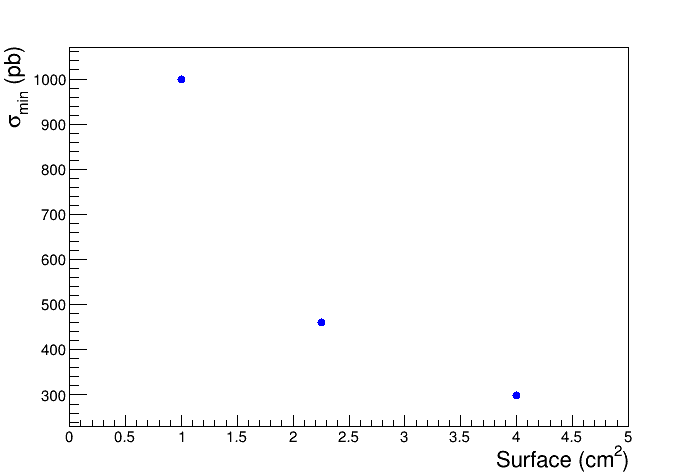
\includegraphics[scale=0.5]{Grafici_Tesi2/Granularitanew/sigma_min.png}
	\caption{L'andamento del rapporto segnale-fondo al variare della superficie del telescopio. Le barra di errore sono più piccole della dimensione del marker.} \label{fig:rapporto_segnale_fondo}
\end{figure}

%Tuttavia, avere superfici più grandi significa anche aumentare il verificarsi del pile-up, in quanto cresce la probabilità che due o più ioni vadano a finire nello stesso rivelatore nella stessa finestra temporale, producendo un segnale somma di due segnali.
Quando si analizzano le condizioni di granularità è opportuno prendere in considerazione anche un altro fenomeno legato alla superficie di rivelazione: il pile-up.
In particolare, se le superfici sono più grandi, cresce la probabilità di pile-up, in quanto diventa più probabile che due o più ioni vadano a finire sullo stesso rivelatore nella stessa finestra temporale, producendo un segnale somma di due segnali.
È stato, dunque, effettuato un calcolo analitico per dedurre la probabilità di pile-up: si ricorda che il rapporto fra la probabilità $\mathcal{P}(> \! 1)$ di avere più di un evento e la probabilità $\mathcal{P}(1)$ di averne uno solo può essere espressa come il seguente rapporto
\begin{equation}
\frac{\mathcal{P}(> \! 1)}{\mathcal{P}(1)} = \frac{1 - 
	\mathcal{P}(0) - \mathcal{P}(1)}{\mathcal{P}(1)}
\end{equation}
Poiché questa tipologia di fenomeni è governata dalla statistica di Poisson, la precedente espressione assume la forma
\begin{equation}  \label{eq:calcolo_pile-up}
\frac{\mathcal{P}(> \! 1)}{\mathcal{P}(1)} = \frac{1 - 
	\mbox{e}^{-\mu} - \mu \,\mbox{e}^{- \mu}}{\mu \, \mbox{e}^{- \mu}}
\end{equation}
laddove $\mu$ indica il valore medio della distribuzione.
Nel caso in esame, tale valore medio non è altro che il prodotto fra la larghezza dell'intervallo temporale $\tau$ e il rate di particelle, con quest'ultima quantità data dal prodotto tra il flusso $\Phi$ di particelle incidenti e la superficie $S$ del rivelatore.
\begin{figure} [!t]
	\centering
	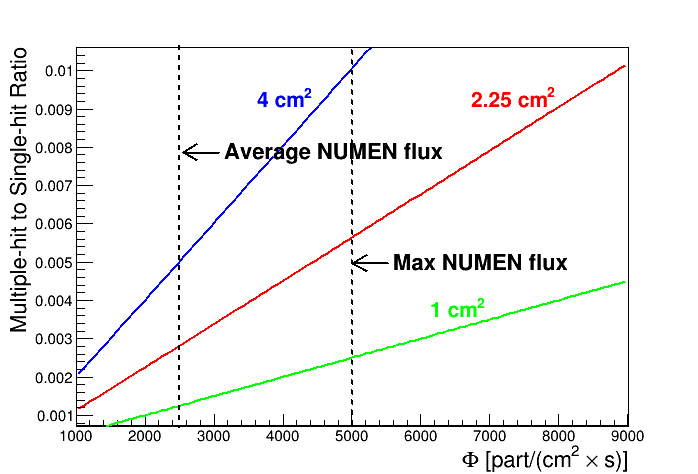
\includegraphics[width=\textwidth, keepaspectratio]{Grafici_Tesi2/Granularita/pile-up3.png}
	\caption{La probabilità di avere eventi di pile-up rispetto alla probabilità di avere un singolo evento al variare del flusso di particelle incidenti e della superficie del rivelatore. Le linee tratteggiate indicano rispettivamente il flusso massimo e medio attesi per NUMEN.} \label{fig:pile-up}
\end{figure}
Dunque, la~\ref{eq:calcolo_pile-up} può essere scritta come
\begin{equation} \label{eq:pile-up}
\frac{\mathcal{P}(> \! 1)}{\mathcal{P}(1)} = \frac{1 - 
	\mbox{e}^{- \tau \, \Phi \, S} - \tau \, \Phi \, S \,\mbox{e}^{- \tau\, \Phi \, S}}{\tau \, \Phi \, S \, \mbox{e}^{- \tau \, \Phi \, S}}
\end{equation} 
Assumendo una finestra temporale della durata di 1~$\mu$s, si è riportato in Figura~\ref{fig:pile-up} l'andamento della~\ref{eq:pile-up} in funzione del flusso di particelle incidenti e della superficie del rivelatore: come si può notare, tale quantità cresce rapidamente all'aumentare della superficie.
Dal momento che i valori riscontrati sono comparabili alle percentuali di contaminazione mostrate in precedenza, il pile-up può rappresentare un serio problema per NUMEN.
Poiché per gli obiettivi del progetto è necessario lavorare con fasci di elevata intensità, bisogna minimizzare la probabilità di pile-up; di conseguenza, la superficie dei telescopi non può essere eccessivamente grande.





%Due aspetti diversi spingono in direzioni opposte: è necessario cercare una situazione di compromesso fra le due esigenze.
%Alla luce delle considerazione svolte, la migliore condizione di granularità sembra essere rappresentata dai telescopi con dimensioni trasversali di 1.5~cm $\times$ 1.5~cm, in quanto riesce ad unire un'alta percentuale di riconoscimento del segnale con una bassa probabilità di pile-up.

Oltre a quelli già citati, nella scelta finale delle condizioni di granularità da adottare entrano in gioco anche altri fattori, legati ad esempio al numero di canali necessari per leggere tutti i dispositivi e alla dissipazione del calore prodotto dai circuiti elettronici.
È chiaro che, se le dimensioni sono più piccole, il numero di rivelatori da utilizzare per riempire la stessa superficie è più grande; di conseguenza, al diminuire della superficie dei telescopi, crescono sia il numero di canali sia il numero di circuiti elettronici.
Ogni circuito, quando è in funzione, produce calore, che deve essere dissipato per evitare il surriscaldamento delle apparecchiature.
Se il numero di circuiti è grande, può essere necessario realizzare un sistema di raffreddamento ad hoc, che richiederebbe ulteriori sforzi di progettazione e costi di produzione.

Dal momento che aspetti diversi spingono in direzioni opposte, è necessario cercare una situazione di compromesso.
Alla luce delle considerazioni svolte, la condizione ottimale di granularità sembra essere rappresentata dai telescopi con dimensioni trasversali di 1.5~cm $\times$ 1.5~cm, in quanto in primo luogo offre un ottimo rapporto S/B e una sensibilità di misura adeguata per lo studio delle reazioni di DCE a bassa energia di eccitazione.
Inoltre, presenta una probabilità di pile-up sufficientemente piccola anche al flusso massimo atteso per NUMEN.
Infine, consente di mantenere su livelli ragionevoli il numero totale di dispositivi e di canali.


%offrono un buon rapporto S/B, che può essere migliorato utilizzando la correlazione $\mbox{tof} - E_{CsI}$, mantengono sufficientemente bassa la probabilità di pile-up e richiedono meno della metà dei dispositivi che occorrerebbero se si utilizzassero i telescopi 1.5~cm $\times$ 1.5~cm.











%Da continuare...
